\documentclass[12pt]{ucsddissertation}
% mathptmx is a Times Roman look-alike (don't use the times package)
% It isn't clear if Times is required. The OGS manual lists several
% "standard fonts" but never says they need to be used.
\usepackage{mathptmx}
\usepackage{cite}
\usepackage{pdflscape}
\usepackage[NoDate]{currvita}
\usepackage{array}
\usepackage[T1]{fontenc}
\usepackage{tabularx}
\usepackage{booktabs}
%\usepackage{caption}
%\captionsetup[figure]{font=small}
\usepackage[font=small,labelfont=bf]{caption}
\usepackage{mathtools, nccmath}
%\usepackage{hyperref}
%\usepackage{dblfloatfix}    % To enable figures at the bottom of page
%\usepackage[demo]{graphicx} % [demo] option for empty figure
%\usepackage{kantlipsum}     % for random text
\usepackage{ragged2e}
\usepackage{subcaption}
\usepackage{amsmath}
\usepackage{microtype}
\usepackage{multicol}
\usepackage[breaklinks=true,pdfborder={0 0 0}]{hyperref}
\usepackage{graphicx}
%\usepackage{subfig}
\usepackage{pdfpages}
\usepackage{siunitx}
%\usepackage[margin=1in]{geometry}
\usepackage{wrapfig}
\usepackage{color,float,amssymb,amsmath}
\usepackage[font=small]{caption, subcaption}
\usepackage [english]{babel}
\usepackage [autostyle, english = american]{csquotes}
\usepackage{verbatim}
\usepackage[version=4]{mhchem}
%\usepackage{chngcntr}
\usepackage{chngcntr}
\counterwithin{figure}{chapter}
\usepackage{chemformula}
\MakeOuterQuote{"}
\AtBeginDocument{%
	\settowidth\cvlabelwidth{\cvlabelfont 0000--0000}%
}

% OGS recommends increasing the margins slightly.
\increasemargins{.1in}
\newcommand\tab[1][1cm]{\hspace*{#1}}
% These are just for testing/examples, delete them
\usepackage{trace}
%\usepackage{showframe} % This package was just to see page margins
\usepackage[english]{babel}
\usepackage{blindtext}
\overfullrule5pt
\bibliographystyle{unsrt}
\newcommand{\schemename}{Scheme}
\newcommand{\listschemename}{List of Schemes}
\newlistof[chapter]{scheme}{los}{\listschemename}
\makeatletter
\ucsd@setuplistof{scheme}{los}\listschemename\schemename\listofscheme
%\makeatother

% ---

% Required information
\title{Multiscale analysis and visualization of biophysical structure and biochemical function with\\ computational microscopy}
%Visualization of biophysical structure and biochemical function in multiple scales \\with computational microscopy}
\author{Sophia P. Hirakis}
\degree{Chemistry \\ with a Specialization in \\ Multiscale Biology}{Doctor of Philosophy}
% Each member of the committee should be listed as Professor Foo Bar.
% If Professor is not the correct title for one, then titles should be
% omitted entirely.
\chair{Professor Rommie E. Amaro}
\cochair{Professor J. Andrew McCammon} % Optional
% Your committee members (other than the chairs) must be in alphabetical order
\committee{Professor Katja Lindenberg}
\committee{Professor Charles L. Perrin}
\committee{Professor Terrence J. Sejnowski}
\committee{Professor Elizabeth Villa}
\degreeyear{2019}

% Start the document
\begin{document}
% Begin with frontmatter and so forth
\frontmatter
\maketitle
\makecopyright
\makesignature
% Optional
\begin{dedication}
\setsinglespacing
\raggedright % It would be better to use \RaggedRight from ragged2e
\parindent0pt\parskip\baselineskip
\begin{center}
\vspace{0.2in}
I am fortunate to have been blessed with two angels, \\who each provided me with one wing so that I could fly.. \\
\vspace{0.2in} 
\textbf{I dedicate this work to my parents}
\vspace{0.1in}
\\ To my beloved father, my baba, \\$\pi\alpha\tau\acute{\epsilon}\rho\alpha$ $\mu$o$\upsilon$ \\ \textit{Petros Emmanuel Hirakis} \\Thank you for being an example of humility and hard work. \\ \vspace{0.1in}
To beautiful mother, my reason, \\ $\mu\alpha\nu$o$\acute{\upsilon}\lambda\alpha$  $\mu$o$\upsilon$\\\textit{Marina (Prearis) Hirakis} \\Thank you for believing in me when I did not believe in myself.\\

\vspace{0.3in}
\textbf{This work is also dedicated to the eternal memory \\of the people that I loved and lost during this journey} \\
\vspace{0.1in}
My grandmother, \textit{Sofia Sotiriou XHPAKH}\\
My grandmother, \textit{Kalliopi Mastromanolis Prearis}\\
My grandfather,  \textit{Minas Emmanuel Prearis}\\
My aunt, \textit{Theodosia Prearis Dargakis}\\
My uncle, \textit{George Dargakis}\\
My koumparo, \textit{Kostas N. Protopapas}\\
My cousin, \textit{Kostas N. Dais}\\
My heroic fighter, \textit{Anthony "Tony" Chester Miller}\\
My father-figure, \textit{George J. Tsimiklis}\\
My favorite musician, \textit{Antonios Nicolaidis}\\
My Johnny boy, \textit{John LaBarbera}\\
My dear friend, \textit{Vasilios N. Diakokomninos}\\
My spiritual brother, \textit{Matthew G. Walker}\\
My sea sister, \textit{Sophia Tiar$\acute{e}$ Bartlow}\\
My fellow villager, \textit{Georgios Nikitas}\\
My beloved chemistry professor, \textit{Brother Andrew Joseph Winka}\\
My fearless microscopy professor, \textit{Gina Sosinsky}\\
and My almost-colleague, \textit{Anushka Michailova}\\

\vspace{0.2in}
 Finally, I dedicate my thesis to the youth of Greece, \\whose future remains bright despite our tribulations\\ and to the everlasting life of the village of\\ \textbf{Olympos, Karpathos}
\end{center}

\end{dedication}


% Optional
\begin{epigraph}
\vskip0pt plus.5fil
\setsinglespacing
{\flushright
I believe there exists, and I feel within me,\\ \textit{an instinct for the truth, or knowledge or discovery,} \\of something of the same nature as the instinct of virtue, \\and that our having such an instinct is \textbf{reason enough}\\ for scientific researches without any practical\\ results ever ensuing from them.
\vskip\baselineskip
\textit{Charles Darwin       }\par}
\vfil
\begin{center}
Scientists may seek Truth,  but\\ \texttt{Science is the Art of Approximation}. 
\\Just as artists use their media to represent the truths they see about the world, \\ we scientists use our equations, models and case studies\\to represent the truth as it has been \textbf{revealed} to us. \\But in those dark weary hours in the dead of night, we acknowledge to \\ourselves that we have provided only a representation of reality, \\ \textit{an approximation of a deeper truth.} \\
\vskip0pt plus.15fil
Our models and conclusions are like shells in which we hope \\to hear an echo of the great ocean beyond.

\vskip\baselineskip
\textit{William Hooke}
\end{center}
\vfil
\noindent When you have a father and a mother \\who work \textbf{all their lives} so you can have\\ an education and build your body - it's a blessing.


\vskip\baselineskip
\hskip0pt\textit{Lou Gehrig}\hskip0pt plus4fil\null

\vfil
\begin{center}
The world breaks everyone..\\
and afterwards,
many are strong at the broken places.

\vskip\baselineskip
\textit{ Ernest Hemingway}
\end{center}

%\vfil
\end{epigraph}

% Next comes the table of contents, list of figures, list of tables,
% etc. If you have code listings, you can use \listoflistings (or
% \lstlistoflistings) to have it be produced here as well. Same with
% \listofalgorithms.
\tableofcontents

% \chapter{List of Symbols and Acronyms}
\clearpage
\begin{center}
LIST OF SYMBOLS AND ACRONYMS
\end{center}
\phantomsection
\addcontentsline{toc}{chapter}{List of Symbols and Acronyms}

{\doublespacing
 \setlength{\parindent}{1pt} 
 
%If using a tabular (especially if shorter than one page)

\noindent\begin{tabular}{@{}l l}
%$\theta$ \\ \footnotesize \centering  angle\\
\si{\angstrom} \tab[5.45cm]Angstrom\\
AP \tab[5.15cm]Action Potential\\
BD \tab[5.15cm]Brownian Dynamics\\
cAMP \tab[4.6cm]Cyclic Adenosine Monophosphate\\
CBD \tab[4.86cm]Cyclic-nucleotide Binding Domain\\
CMDN\tab[4.54cm]Calmodulin\\
CRU \tab[4.74cm] Calcium Release Unit\\
Cryo-EM \tab[4.09cm]Cryo-Electron Microscopy\\
C4BP \tab[4.6cm] Human C4b-Binding Protein\\
GAS \tab[4.76cm] Group A \textit{Streptococcus}\\
H/DxMS \tab[4.05cm] Hydrogen/Deuterium Exchange Mass Spectrometry\\
LTCC\tab[4.8cm]L-Type Calcium Channel\\
HVR \tab[4.7cm]  Hyper-Variable Region\\
MD \tab[5cm]Molecular Dynamics\\
MSM \tab[4.7cm]Markov State Model\\
NCX \tab[4.7cm] Na\textsuperscript{+}/ Ca\textsuperscript{2+} exchanger\\
ODE \tab[4.84cm]Ordinary Differential Equation\\
PDE \tab[4.87cm]Partial Differential Equation\\
PKA \tab[4.85cm]Protein Kinase A\\
PMCA \tab[4.5cm]Plasma Membrane Ca\textsuperscript{2+} ATPase\\
RyR \tab[4.9cm]Ryanodine Receptor\\
SAXS \tab[4.6cm]Small-Angle X-ray Scattering\\
SERCA \tab[4.33cm]Sarco/Endoplasmic Reticulum Calcium-ATPase\\
TT \tab[5.15cm]Transverse Tubule\\
WT \tab[5.02cm]Wild-Type\\


\end{tabular}

\bigskip %% ignore this; just to add some space between the tabular and the next text

%If using a description list:

%\begin{description}
%\item[$\theta$] the temperature
%\item[ABC] a clever acronym
%\end{description}
}

\listoffigures
\listofscheme
\listoftables


% Preface
\begin{preface}
I begin this thesis with a feeling of mischievous satisfaction. As a child, I trained as an actor and learned to improvise in order to evoke emotion in my audience. This was my coping mechanism, of sorts, for an awkward and over-zealous personality. But, at my core, I am \textbf{an artist.} The truth is that during the course of my life, I fooled \textit{a lot} of people into thinking that I was scientist and not an artist, including myself. 

I sang before I could speak, danced before I could walk, and played with anything made sound. Music was not explicitly encouraged by my father. To buy my first guitar, he encouraged me to save my money and I did so, buying it myself at the age of 13 with money that I earned from tutoring.  $\Pi\acute{\epsilon}\tau\rho$o$\varsigma$, my father, pushed me towards a career in medicine and I studied hard in order to appease him. From my father, I inherited a thirst for challenges and expanding my boundaries which allowed me to excel, and from my grandfather, M$\eta\nu\acute{\alpha}\varsigma$ an obsession with music, which distracted me fully. My grandfather was not fondest of my educational pursuits, offering marriage as the "logical" solution. But my mother and grandmother pushed me to continue with my education to achieve the dreams that they could never achieve. 

In our village, $\acute{O}\lambda\upsilon\mu\pi$o$\varsigma$ \textit{K}$\alpha\rho\pi\acute{\alpha}\theta$o$\upsilon$, more than 80\% of women never complete high school. This meant that my grandmother longed for an education that she never had the opportunity to have. Despite this precedent, my grandmother always encouraged me to pursue my education. My mother was married with a child at the age of 21, and she never completed college either. My grandfather never learned to formerly read and write in an academic sense, and my father never completed grade school. I had no precedent, but I \textit{did} have encouragement,  

Having gone to school in Greece during my early years and Greek schools throughout my primary education, the Socratic method-dialogue, also known as "conversational learning" or "learning with interruptions" was common. But my tendency towards hyper-stimulation always caused me to ask "too many questions." Most American teachers found it disruptive, but in the 9th grade, Ms. Primm asked me to stay after class; what I thought would be some form of reprehension to which I was accustomed. Instead, she told me that I "asked the best questions that [she] ever heard from a student." She encouraged me to become a scientist too, instilling within me the most important thing I've carried throughout my educational career: belief in myself. She was the first person that made me see myself as a scientist and helped me begin a journey that began with biology, seeded in chemistry, and flourished with physics.

My love affair with physics began at 4 AM on a June summer night of 2012, while laying on a couch in Baltimore, MD, USA.  Exhausted from his shift at Hilltop Carry-out, my $\sigma\upsilon\gamma\chi\omega\rho\iota\alpha\nu\acute{o}\varsigma$ \textit{E}$\lambda\upsilon\mu\pi\acute{\iota}\tau\eta\varsigma$ (fellow villager of Olympos) and dear friend Minas Giorgakis laid in his bed and put on a documentary for me to watch \textit{about the mysteries of the universe} in hopes of occupying me enough so that he could get some sleep.  
\begin{center}
I fell deeply in love. 
\end{center}

The vastness of the universe humbled me. The mere idea of combining chemistry with physics excited me. Just a year before, I was awarded a Bachelors degree in Biochemistry from Manhattan College, and was admitted to the PhD program at the University of California, San Diego, my dream school. After \textit{bearing witness to} the vastness of the universe, I found myself looking for professors to work with in the department that studied cosmic chemistry. I quickly changed my mind when I realized that those beautiful fly-through images of space took decades to systematically study and acquire knowledge about. I was reminded of the advice of my beloved Physical Chemistry professor, Jianwei Fan, PhD: "\textit{Sophia, stick to your strengths.}"\\


At first, I was offended by Dr. Fan's suggestion that I stick to the study of organic chemistry, though I admittedly had intuition for synthesis. The Greeks have a word for my response: $\pi\varepsilon\acute{\iota}\sigma\mu\alpha$ (pe$\acute{i}$zma). I encourage the reader to decide upon a definition for this poly-semantic word. With $\iota\sigma\chi\upsilon\rho$o$\gamma\nu\omega\mu$o$\sigma\acute{\upsilon}\nu\eta$ (ishchyrognomos$\acute{i}$ni), a bull-headed will and stubbornness, I decided I would take the middle road, combining my love for biochemistry with my thirst to understand why we observe what we do, in the study of biophysics.\\
\tab[0.7cm]I packed up my life in my 2007 Spyder Eclipse named "Angie" after the legendary Rolling Stones song and along with my best friend, Yianna (Rodriguez) Zois, took off on a ten day adventure to go to the place I always wanted to be, San Diego, California, USA. The brisk air, the green mountains; those sandy valleys and glorious sunsets of San Diego acted as a mere substitute for the place which I had never been able to call home, my beloved Karpathos.\\
\tab[0.7cm]In retrospect, I  sometimes wish I \textit{had} listened to Dr. Fan. I often wish that I took Dr. (Kyriacos Costas) K.C. Nicolaou's invitation to join his lab at Scripps. I would have likely finished my PhD earlier, since I had a strength for synthesis; but the number of gray hairs in exchange for total synthesis over biophysics might never be known. \\
\tab[0.7cm] But something drew me to biophysics--the ability to "see" what I learned about as a biochemist. Using mathematically-accurate artistic and computational approximations of proteins and cells, I could finally fully understand the concepts that Dr. Chiara Indiani drilled deep into my mind. It felt intuitive to examine proteins and see how their secondary structure was disrupted by molecular motions. The challenges, however, were more than I anticipated.\\
\tab[0.7cm]The learning curve for biophysics was \textit{incredibly} steep. In addition to the complexities of the mathematics I was learning, I suffered endlessly by exchanging "a" with $\alpha$ and "b" with $\beta$, a pain that my beloved professor Katja Lindenberg found comical, since Greek is my first language. But at the end of statistical mechanics, I had the pleasure of understanding the elegance with which quantum mechanics and physical chemistry describe molecular motion with each integration of each time step. This, "mathematical magic" coupled with my ability to visualize the biophysical implications of system alterations on the level of the protein convinced me that I was on the right path.  I had my heart set on biophysical chemistry, but still I yearned for more. I yearned to apply my understanding of biochemistry to the complexities of diseases.\\
\tab[0.7cm]Early on in my life, I developed a kind of \textit{obsession} with identifying and understanding illnesses. This started as soon as I could read. My mother had a book by H. Winter Griffith called "A Complete Guide to Pediatric Symptoms, Illnesses and Medications." I would often find myself correlating  my siblings' symptoms to illnesses suggesting doctors visits, way before WebMD was a thought. My curiosity blossomed in my later years as I learned more about biology and the ways that mutations lead to phenotypical differences that cause diseases; diseases that I would one day witness the real effects of.\\
\tab[0.7cm]In college, I worked for three years in the Department of Surgery Research at Johns Hopkins University Bayview Medical Center. In partnership with the Firefighters Association of Baltimore, MD, we aimed to treat burn wounds on animals and humans with the use of protein cocktails. As a biochemist interested in serious medical conditions, this fascinated me--the concept that small proteins (nm) could heal damaged tissues for the regeneration of skin cells to form collagen and hair follicles to generate $\alpha$-keratin. I later worked in the Department of Surgical Pathology at Montefiore Medical Center where I dissected human organs. Morbid, I know but I worked with diseased organs daily, trying to understand \textbf{why} patients were sick. It was here that I learned the true meaning of multiscale biochemistry. 

Like true scientists, after receiving any surgically removed organ during or after surgery, we followed a very strict protocol. The organ would be measured, visually described, and the description dictated to a computer directly into a pathology report. The organ would be fixed in a fixation agent, like formaldehyde, in order to preserve the ultrastructure of the specimen. Successive dissections dependent on the tissue type would be made until an interesting characteristic was identified. This could be, for instance, a calcification of tissue or necrosis of a major artery. My job was to identify the morphology of the disease on the cellular level using a light microscope. In this way, the multiscale nature of disease was revealed to me. 

This experience sparked within me a desire to understand the cause of diseases. In graduate school, my advisor, Dr. Rommie E. Amaro gave me an opportunity to do just this in a way that I could have never imagined. Using a unique set of computational tools, I have learned to tease out the factors that underlie diseases. The most satisfying part of this experience is the use of tools that allow you to visually interpret the results of our experiments. 

\end{preface}


\begin{acknowledgements}
I would like to acknowledge .. .. .. 

Chapter 1, in full, is a reprint of the material as it appears in Frontiers in Physiology 2015. 
Boras, Britton W.; \textbf{\underline{Hirakis, Sophia P.}}; Votapka, Lane W.; Malmstrom, Robert D.; Amaro, Rommie E.; McCulloch, Andrew D.;"Bridging scales through multiscale modeling: a case study on protein kinase A," Frontiers in Physiology, 6: 250, 2015. 
 The dissertation author was the co-primary author of this paper.

Chapter 2, in full, is pre-publication print of an article published in Nature Microbiology 2016. 
Buffalo, Cosmo Z.; Bahn-Suh, Adrian J.; \textbf{\underline{Hirakis, Sophia P.}}; Biswas, Tapan; Amaro, Rommie E.; Nizet, Victor; Ghosh, Partho; "Conserved Patterns hidden within group A Streptococcus M protein hypervariability are responsible for recognition of human C4b-binding protein." The dissertation author was the third author of this paper.

Chapter 3, in full, is a reprint of the material as it appears Biochemistry 2017. 
\textbf{\underline{Hirakis,}}\ \textbf{\underline{Sophia P.}}; Malmstrom, Robert D.; Amaro, Rommie E.; "Molecular Simulations Reveal an Unresolved Conformation of the Type IA Protein Kinase A Regulatory Subunit and Suggest its Role in the cAMP Regulatory Mechanism." The dissertation author was the primary investigator and author of this paper.

Chapter 4, in part is currently being prepared for submission for
publication of the material. \textbf{\underline{Hirakis, Sophia P.}};  Bartol, Thomas M.; Sejnowski, Terrence, J; Amaro, Rommie E; The dissertation author was the primary investigator and author of this material.




\end{acknowledgements}

%Vita goes next
\begin{vita}
\noindent
\begin{cv}{}
\begin{cvlist}{}
\item[2011] Bachelor of Science in Biochemistry, Manhattan College, Riverdale, NY
\item[2012-2015] Teaching Assistant, Department of Chemistry and Biochemistry\\University of California San Diego
\item[2012-2015] Master of Science in Chemistry, University of California San
Diego
\item[2012-2019] Research Assistant, University of California San
Diego
\item[2019] Doctor of Philosophy in Chemistry, University of California San
Diego
\end{cvlist}
\end{cv}

% This puts in the PUBLICATIONS header. Note that it appears inside
% the vita environment. It is optional.
\publications

\noindent \textbf{\underline{Hirakis, Sophia P.}}; Bartol, Thomas M.; Sejnowski, Terrence J.; Amaro, Rommie E.; "Molecules to Membranes: The Calcium Release Unit." Biophysical Journal, 2018, 114(3),  pp. 118a.

\noindent \\ \textbf{\underline{Hirakis, Sophia P.}}; Malmstrom, Robert D.; Amaro, Rommie E.; "Molecular Simulations Reveal an Unresolved Conformation of the Type IA Protein Kinase A Regulatory Subunit and Suggest its Role in the cAMP Regulatory Mechanism." Biochemistry, 2017, June 29; 56 (30), pp 3885-3888.

\noindent \\McCullagh, James V. and \textbf{\underline{Hirakis, Sophia P.}}; "Synthesis of the Commercial Fragrance Compound Ethyl 6-Acetoxyhexanoate: A Multistep Ester Experiment for the Second-Year Organic Laboratory." Journal of Chemical Education, 2017, June 29; 94 (9), pp 1347-1351.

\noindent \\Buffalo, Cosmo Z.; Bahn-Suh, Adrian J.; \textbf{\underline{Hirakis, Sophia P.}}; Biswas, Tapan; Amaro, Rommie E.; Nizet, Victor; Ghosh, Partho; "Conserved Patterns hidden within group A Streptococcus M protein hypervariability are responsible for recognition of human C4b-binding protein." Nature Microbiology, 2016, September 5; 1:16155.

\noindent \\Boras, Britton W.; \textbf{\underline{Hirakis, Sophia P.}}; Votapka, Lane W.; Malmstrom, Robert D.; Amaro, Rommie E.; McCulloch, Andrew D.;"Bridging scales through multiscale modeling: a case study on protein kinase A." Frontiers in Physiology, 2015, September 9; 6:250.

\noindent \\Keating, Tedd; \textbf{\underline{Hirakis, Sophia P.}}; McBride, Nicole; "Perceiving the center of Human Figures." Proceedings and Abstracts of the Annual Meeting of the Eastern Psychological Association, March 6, 2012; vol 81, pp s97.

\noindent \\ Friedenberg, Jay D.; Keating, Tedd; \textbf{\underline{Hirakis, Sophia P.}}; Toscano, Lisa; "The Effects of a Typical In-season Practice Session on Peak Ground Forces and Select Kinematic Variables in Women's Division I Basketball Players." Journal of Strength and Conditioning Research, February, 2012; vol 23, pp 87.
\vspace{5mm}


% This puts in the FIELDS OF STUDY. Also inside vita and also
% optional.
\fieldsofstudy
\noindent Major Field: Chemistry and Biochemistry (Specialization in Multiscale Biology)
\vskip\baselineskip
Studies in Biophysical Chemistry\par
Professor Rommie E. Amaro
\vskip\baselineskip
Studies in Computational Biology\par
Professor Terrence J. Sejnowski


\vskip\baselineskip
\noindent Major Field: Surgery and Medicine
\vskip\baselineskip
Studies in Surgical Research\par
Professors Guy Marti, M.D., John Harmon, M.D.
\vskip\baselineskip
Studies in Emergency Medicine and Toxicology\par
Professor Joseph LaMantia, M.D.

\vskip\baselineskip
\noindent Major Field: Synthetic Chemistry and Chemical Education
\vskip\baselineskip
Studies in Synthetic Organic Chemistry\par
Professor James V. McCullagh, Ph.D.

\vskip\baselineskip
\noindent Major Field: Kinesiology and Cognitive Perception
\vskip\baselineskip
Studies in Kinesiology\par
Professor Tedd Keating, Ph.D.
\vskip\baselineskip
Studies in Cognitive Perception\par
Professor Jay D. Friedenberg, Ph.D.


%\vskip\baselineskip
%Studies in Mechanics\par
%Professors Epsilon Zeta and Eta Theta
%\vskip\baselineskip
%Studies in Electromagnetism\par
%Professors Iota Kappa and Lambda Mu
\end{vita}


%~~~~~~~~~~~~~~~~~~~~~~~~~~~~~~~~~~~~~~~~~~~~~~~~~~~~~~~~~~~~~~~~~%
 

% Put your maximum 350 word abstract here.
\begin{dissertationabstract}
\vspace{0.3pt}

The evasive source and cause of a disease is oftentimes \textit{smaller than you think}. Imagine, though, chasing something that you can't actually \textit{see}. Fortunately for the modern-day biomedical scientist, computational tools harnessing the power of physics using the language of mathematics are able to \textit{see the invisible}. Computational microscopy is a tool developed to visualize the energetic behavior of biological systems. With progressive advancements in computer graphics and the development of mathematical theories to explain biological behavior, computational microscopy has become a useful tool used by many kinds scientists over the greater half of the last century to understand the energetic underpinnings of a system's behavior. Unlike most "microscopes," it allows us to visualize extremely small entities like atoms, molecules, proteins, and cells. More importantly, it allows us to spatiotemporally transcend scales to understand the dynamics of our systems. Like a biophysically detailed time-lapse, we are able to \textit{see through time}, to understand chemical "butterfly effects" that transcend the time and space scale at which they operate. In this thesis, the computational microscope is applied to multiple systems to \textit{visualize and analyze} the physicochemical mechanisms that underlie biological function. Specifically, the thesis is centered on the structure of proteins and subcellular mechanisms driving cardiac function and dysfunction. In the first chapter, we address the concept of multiscale biological simulations, integrating information from atomistic scales toward cellular models of Protein Kinase A. The second chapter demonstrates the ways that atomistic simulations can be applied to the study of the structural interactions in protein-protein complexes vital to the infectious mechanisms of Group-A \textit{Streptococcus}. In the third chapter, two scales of biological simulation are used in tandem to understand the structure and the kinetic behavior of Protein Kinase A RI$\alpha$. The final chapter incorporates the kinetic understanding of relevant species in a realistic subcellular geometry to investigate signaling mechanisms that underlie calcium activation in healthy and diseased hearts. Particular attention is paid to the way that structural alterations on the atomistic, molecular, and membranous level alter the behavior of biological systems. Holistically, this thesis is centered on the use of computational tools and the development of realistic models that can reproduce experimental findings and predict the behavior of systems, driving the creation of new hypotheses. 

\end{dissertationabstract}

% This is where the main body of your dissertation goes!
\mainmatter

%~~~~~~~~~~~~~~~~~~~~~~~~~~~~~~~~~~~~~~~~~~~~~~~~~~~~~~~~~~~~~~~~~%


%  Introduction
\begin{dissertationintroduction}
%\counterwithin{figure}{section}
\counterwithin{equation}{chapter}

The Greek word, $\pi$o$\lambda\upsilon\sigma\acute{\eta}\mu\alpha\nu\tau\alpha$ (poly-s\^em-anta, english: polysemantic) translates to the phrase: a symbol or word that has multiple meanings. Depending on where accents are located in Greek and other accented languages, the meaning of a word can change completely. As such, words can be misinterpreted when translating from one language to another, especially because of the sociological implications of the passage of time. From this phenomenon stems so much of the world's fascination with science: the cycle of observation and theoretical inquiry. Curious minds have learned \textit{simply} that words cannot properly encapsulate the meaning of something fully. Rather, it is \textit{feeling and bearing witness} that satisfies the understanding that the mind craves. 

A language exists, which is not subject to misinterpretation of translation, and that is the language of mathematics. From the first known records of mathematics which date back to approximately 3000 B.C.E. until now, what has been common between four sheep and four goats has always been their \textit{value}, equaling to 4. With common units of length, time, volume and the like, we can describe in exponential terms the quantitative \textit{scale} of a value. Using mathematics, humans can describe observable phenomena--from the attractive forces that govern the behavior of the smallest atom, to the revolution of planets in galaxies that are not our own. What is more, mathematics allows us to tease out simple formulas that \textit{predict} the future state of a system. In simple terms, mathematics is used to encode, translate, and communicate \textit{energy}.

To understand the power of mathematics, we must lend some consideration to the ability to \textit{visualize} energetic concepts. This concept is best demonstrated by one of the most amazing phenomenon known to mankind: the musical genius of Beethoven, \textbf{a deaf man}. How could it be possible for a man who could not \textit{\textit{hear sound}} to produce such melodic masterpieces? The answer is simply, his ability to visualize sound energy. Ludwig van Beethoven once said, 

\begin{center}
    "I always have a \textit{picture in my mind} when composing, and follow its lines."
\end{center}

Ludwig van Beethoven was able to see and feel the mathematical and energetic relationship of musical notes relative to one another, even though he could not hear them. His words allude to the existence of a phenomenon that so many non-traditional artists and scientists live: a deepened understanding of something is somehow tied to ones ability to \textit{feel it, and visualize it} in their mind's eye. The famous mathematician, James Joseph Sylvester once said, 

\begin{center}
    "The musician feels mathematics, the mathematician thinks music: \\ music the dream, mathematics the working life."
\end{center}

\begin{figure}
\centering
        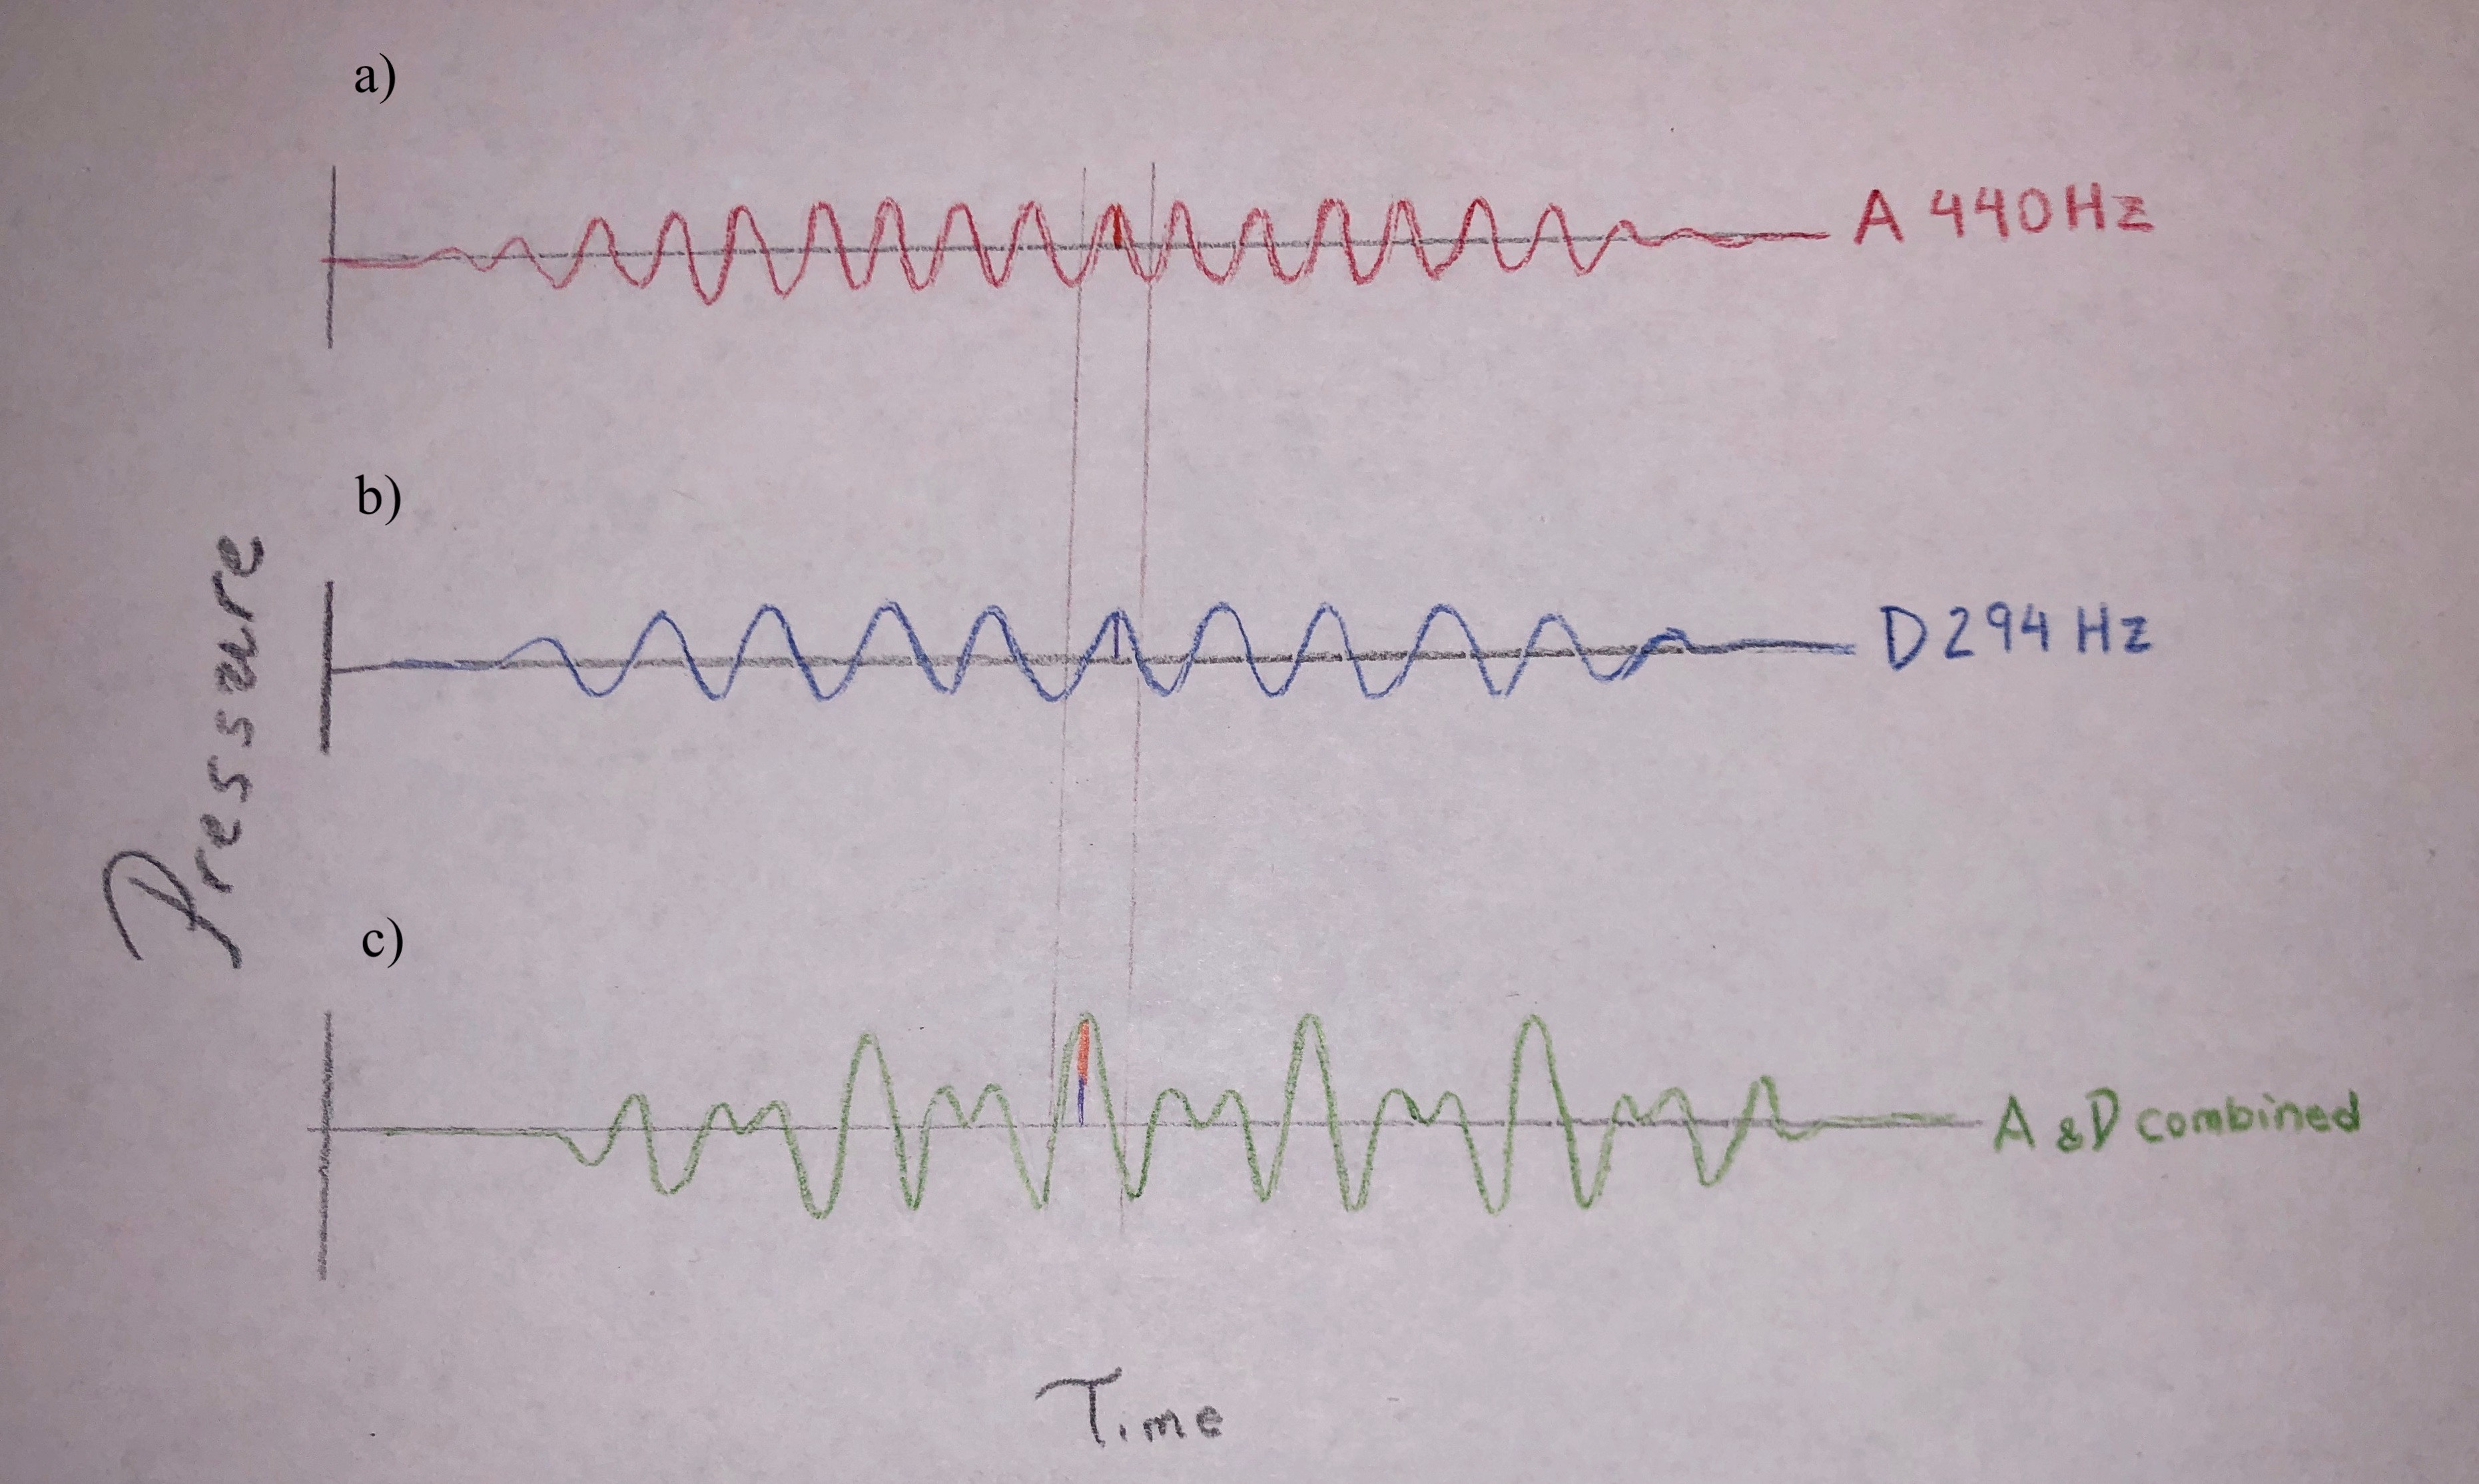
\includegraphics[scale=0.1]{frequencies.jpeg}
        \caption{A drawing of musical frequencies}
        \subcaption{ A drawing of the high frequency, 440Hz musical note,"A" or "La" (red);\textbf{(b)} A drawing of the lower frequency, 294Hz musical note,"D" or "Re" (blue);\textbf{(c)} A drawing of the additive frequencies of "A" and "D" to produce an complex wave function; Adapted from freely available lessons by 3Blue1Brown.}
\label{fig:frequencies of music}
\end{figure}

Many of us do not know what it means to "visualize" energy, music, or mathematics. But, if you have the ability to hear sound, you may recognize the note commonly known as "A" or "La." If you used a pressure reader near the source of the note, the pressure recorder would record 440 energetic detections per second, or 440 Hz (see figure 0.1a). Lower frequencies like the note "D" or "Re" at 240 Hz have longer wavelengths (see figure 0.1b). One can infer that the "lines" that Beethoven referred to are the amplitudes of the sound frequencies. 

If you have ever played a musical instrument, you may already know that these notes compliment each other nicely, a phenomenon known in music as a "harmonious interval." Practically, this means when the two sound waves interact, their waves sum to produce a complex wave (see figure 0.1b). This is but one example of how mathematics and art can be used to \textit{visualize} a physical phenomenon best described by the senses.

This begs the question: how is one able to perceive the energies that surround them? The answer is quite complex but can be simplified with the following explanation: biological organisms are \textit{\textbf{master detectors}}. Every organism, from single-celled bacteria to humans, to organisms that have yet to be discovered living in the deepest oceans and the highest peaks, have the ability to detect energetic changes in their environment in some form or another. 

With properly functioning sensory faculties, we are able to perceive and interpret the energies around us, allowing us to respond to stimuli, learn, and adapt to our environment. This process, however, only works for phenomena that can be observed--at frequencies and energies that can be detected by our sensory systems. More often than not, interesting phenomena are too small/fast and large/slow to be observed and interpreted without aide of technology. Fortunately, the language of mathematics can be used to describe many observable and non-observable phenomena, allowing for contextualization and understanding by inquisitive minds.

\section{Scaling up through the sciences}
As noted earlier, our knowledge and understanding of the world around us is timelessly encoded in the language of \textit{mathematics}. The application of mathematics to the laws that govern the physical world is termed, \textit{physics}. The laws and theories of physics applied to the study of matter are collectively, \textit{chemistry}. The use of chemical principles used to describe living systems is \textit{biochemistry}. All of these disciplines are common in their use of mathematics to prove the principles that are upheld by what we are able to observe through our senses and detect with technology. 

Oftentimes, biological systems are too complex, and detailed mathematical descriptions of them become difficult to compute by hand. For this, scientists use computational algorithms that describe and predict behaviors. But the more explicit we become in describing a system, the more computational power we use. In 1965, Gordon Moore published a paper entitled, "Cramming more components onto integrated circuits," \cite{Moore1965} where he first theorized about the relationship between the passage of time and the growth of computational power, known today as Moore's law. Over half a century later, our technology has grown to a point where almost every person carries a small, powerful computer in their pocket that gives them access to volumes of up-to-date information at the mere decision of the user. Though computation is at its most advanced state to date, biological systems operate so fast and at such small time intervals, that computational power is often the limiting factor in obtaining an answer to questions that go beyond the spatiotemporal scale in question.

Nevertheless, using our currently available technology combined with sophisticated mathematical algorithms, we computational biophysicists have collectively created a powerful tool, \textit{the computational microscope}. Like a true microscope, we can choose a "magnification" or scale to visualize that which we seek to see. Using innovative methods for artistic rendering of atoms, proteins, and cells, the invisible suddenly becomes visible. Most importantly, we can see the biophysical ramifications of small changes that scale upwards, a biophysical butterfly effect.

With humility, I ask the reader: join me in this journey across scales of microscopic biophysical space-time to see the unseen, through the lens of the computational microscope. 

\section{The multiscale nature of biochemistry}

The complexity of biological systems stems from the various scales of space and time at which they operate. In terms of the field of biochemistry, there are many levels that operate in unison to produce an observable phenomenon. This section will describe the various mechanisms that underlie structure in biochemical systems.

\setcounter{figure}{1}
\begin{figure}
%\centering
	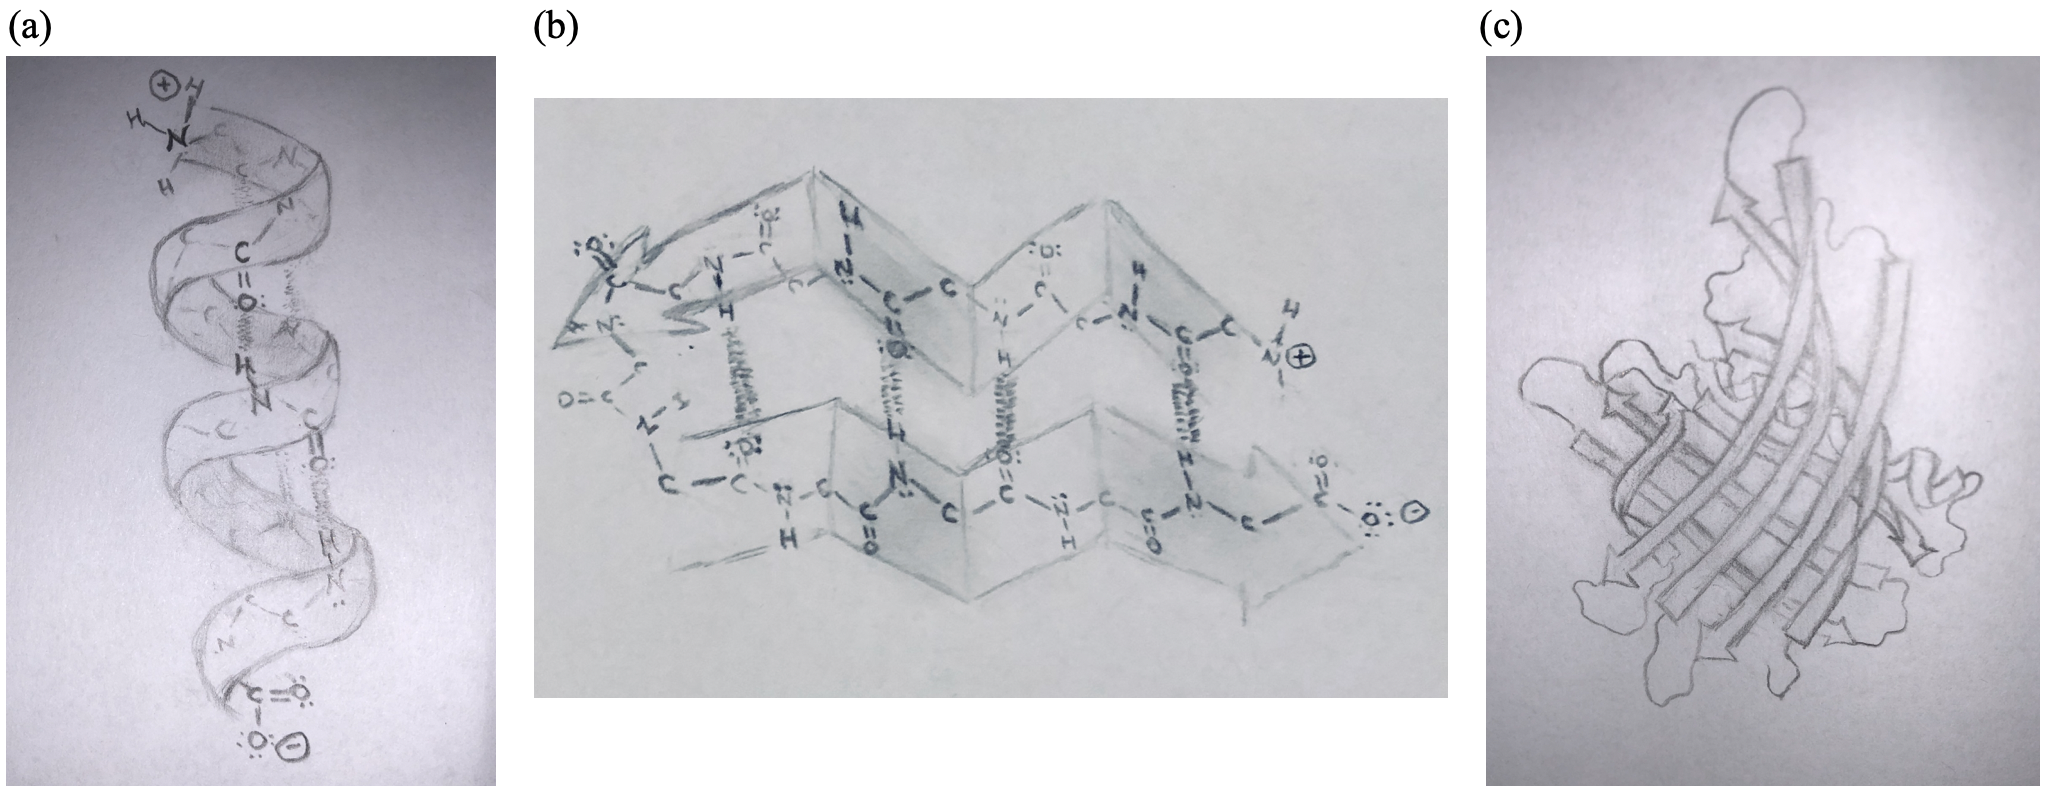
\includegraphics[scale=0.43]{Levels.png}
	\caption{Levels of protein structure}
	\subcaption{$\alpha$-helix structure;\textbf{(b)} Parallel $\beta$-sheet structure; \textbf{(c)} Tertiary structure of a protein comprised of $\beta$-barrels and an $\alpha$-helix}
\label{fig:levels} 
\end{figure}
\begin{comment}
\begin{wrapfigure}{r}{.45\textwidth}
    \begin{minipage}{\linewidth}
    \centering
    \captionsetup[subfigure]{justification=centering}
    \captionsetup[caption]{justification=centering}
    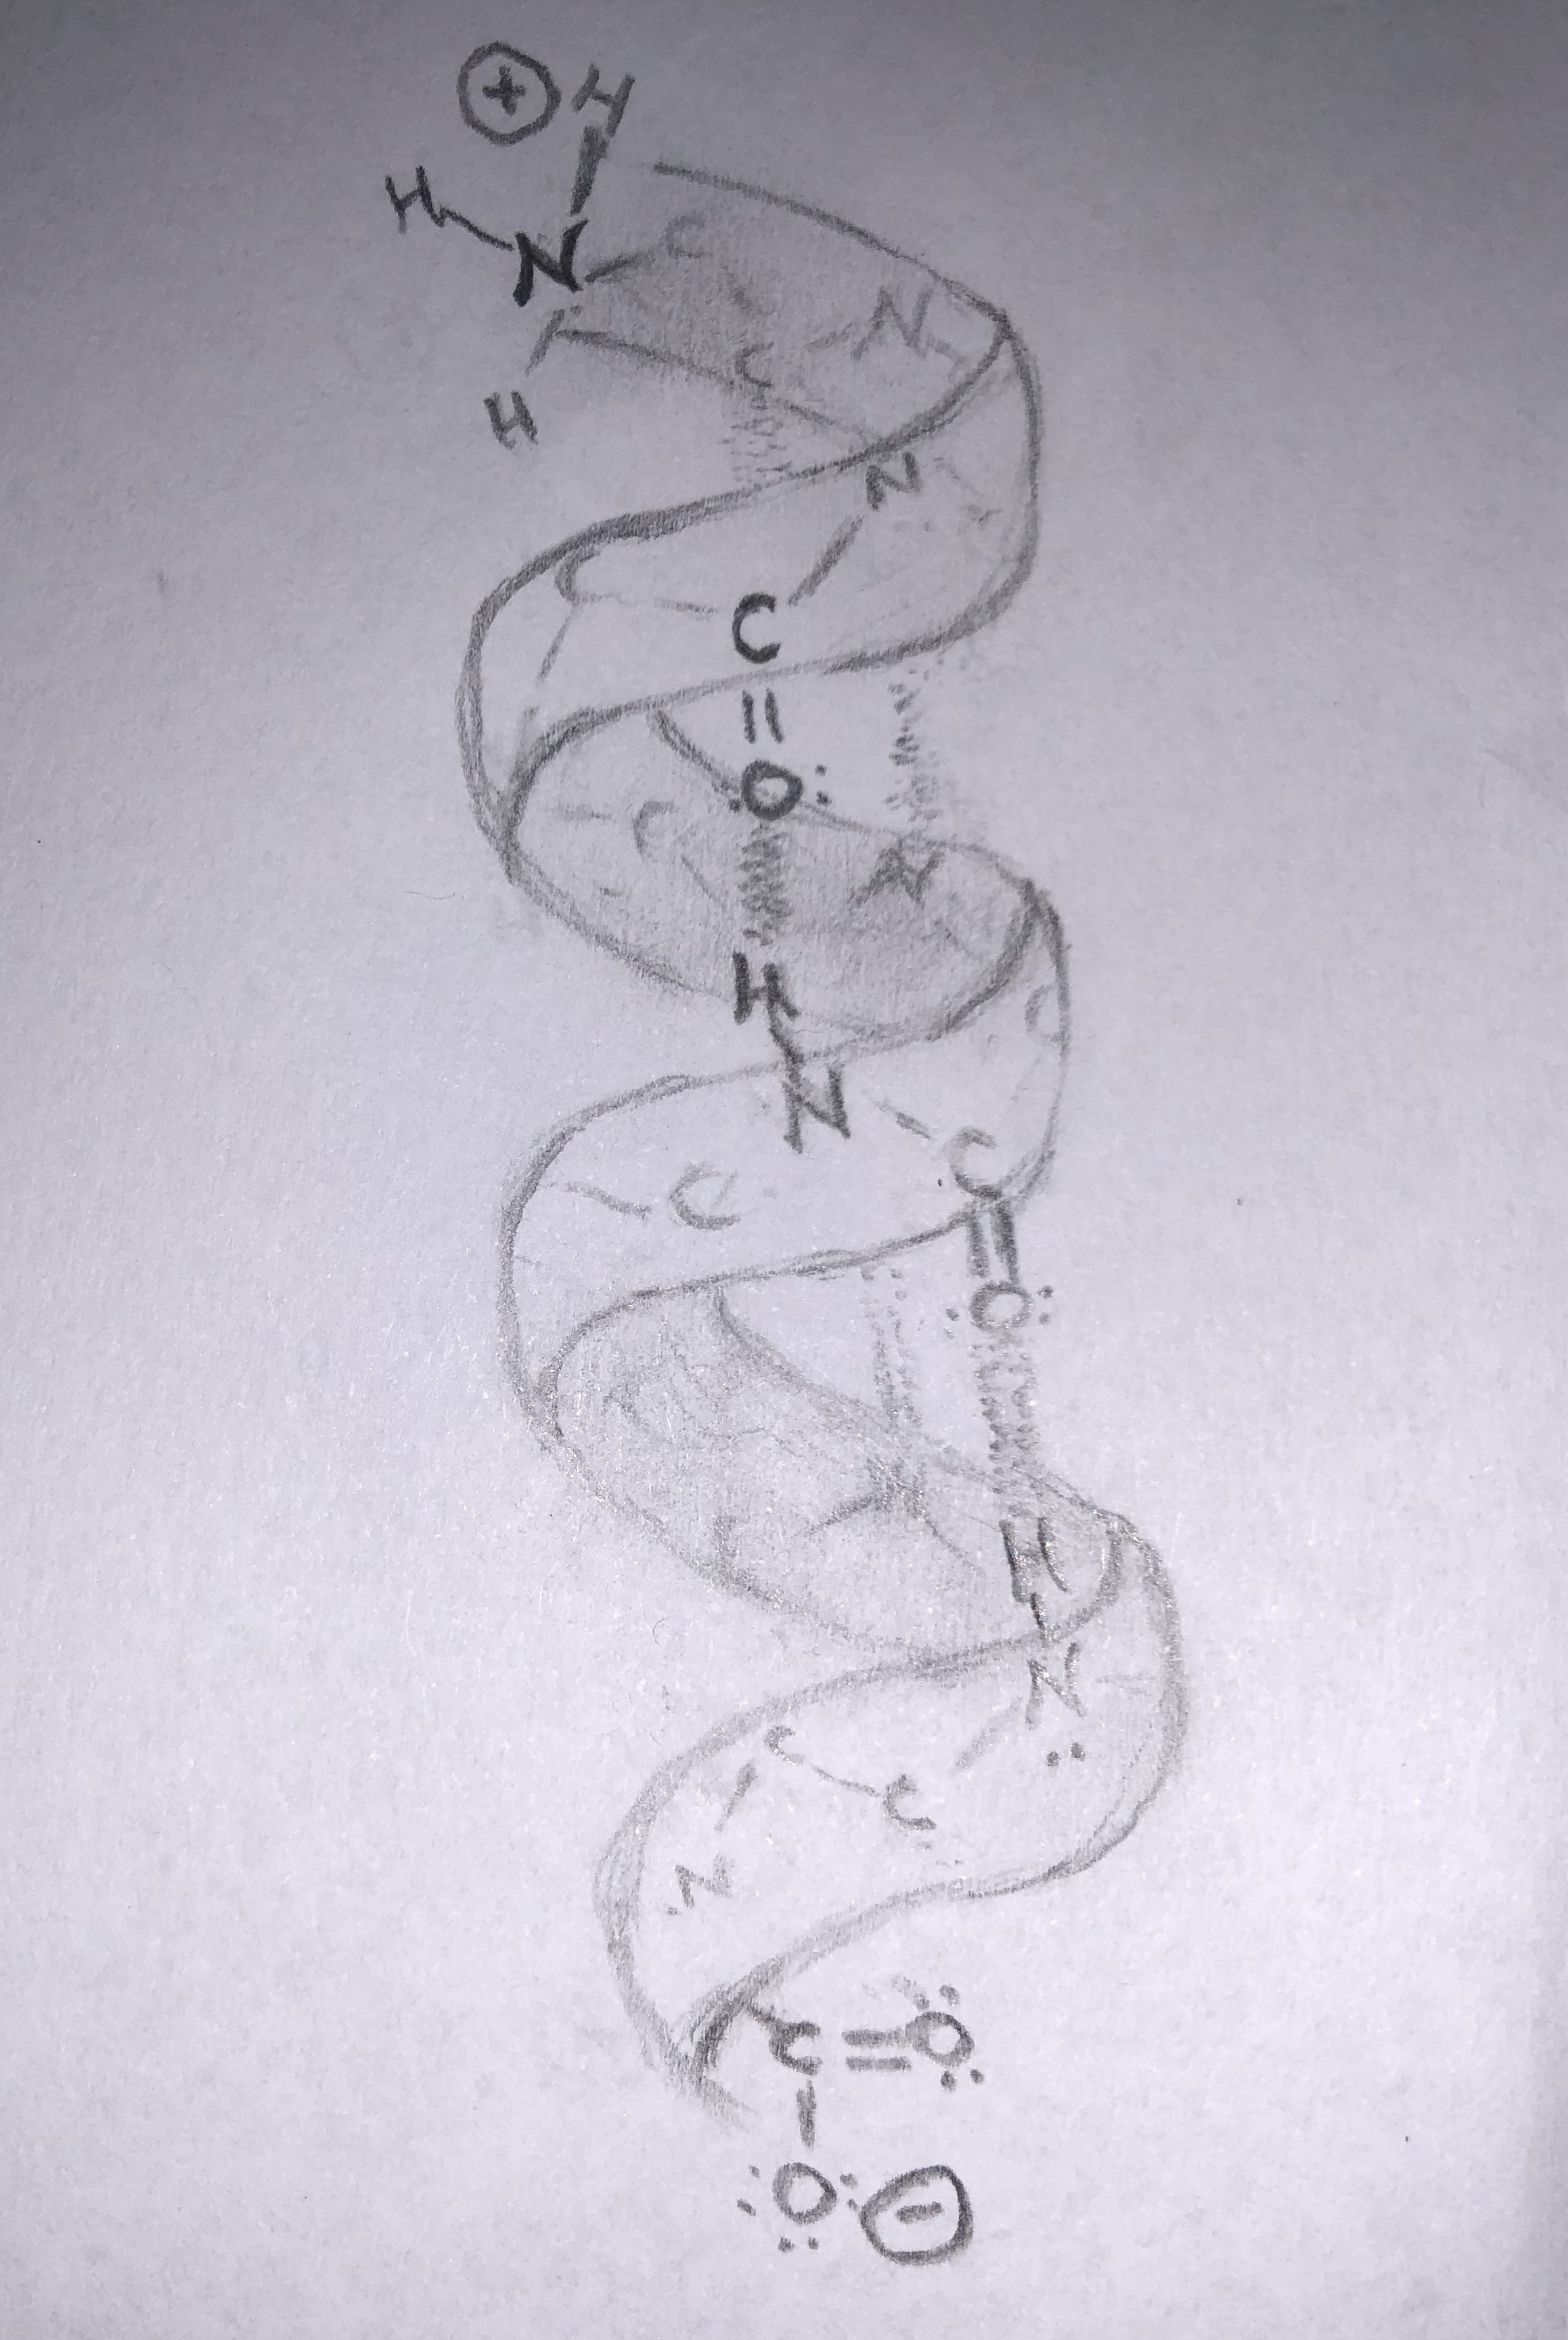
\includegraphics[width=0.55\linewidth]{helix0.jpg}
    \subcaption{$\alpha$-helix structure}
    \label{fig:0a}\par\vfill
    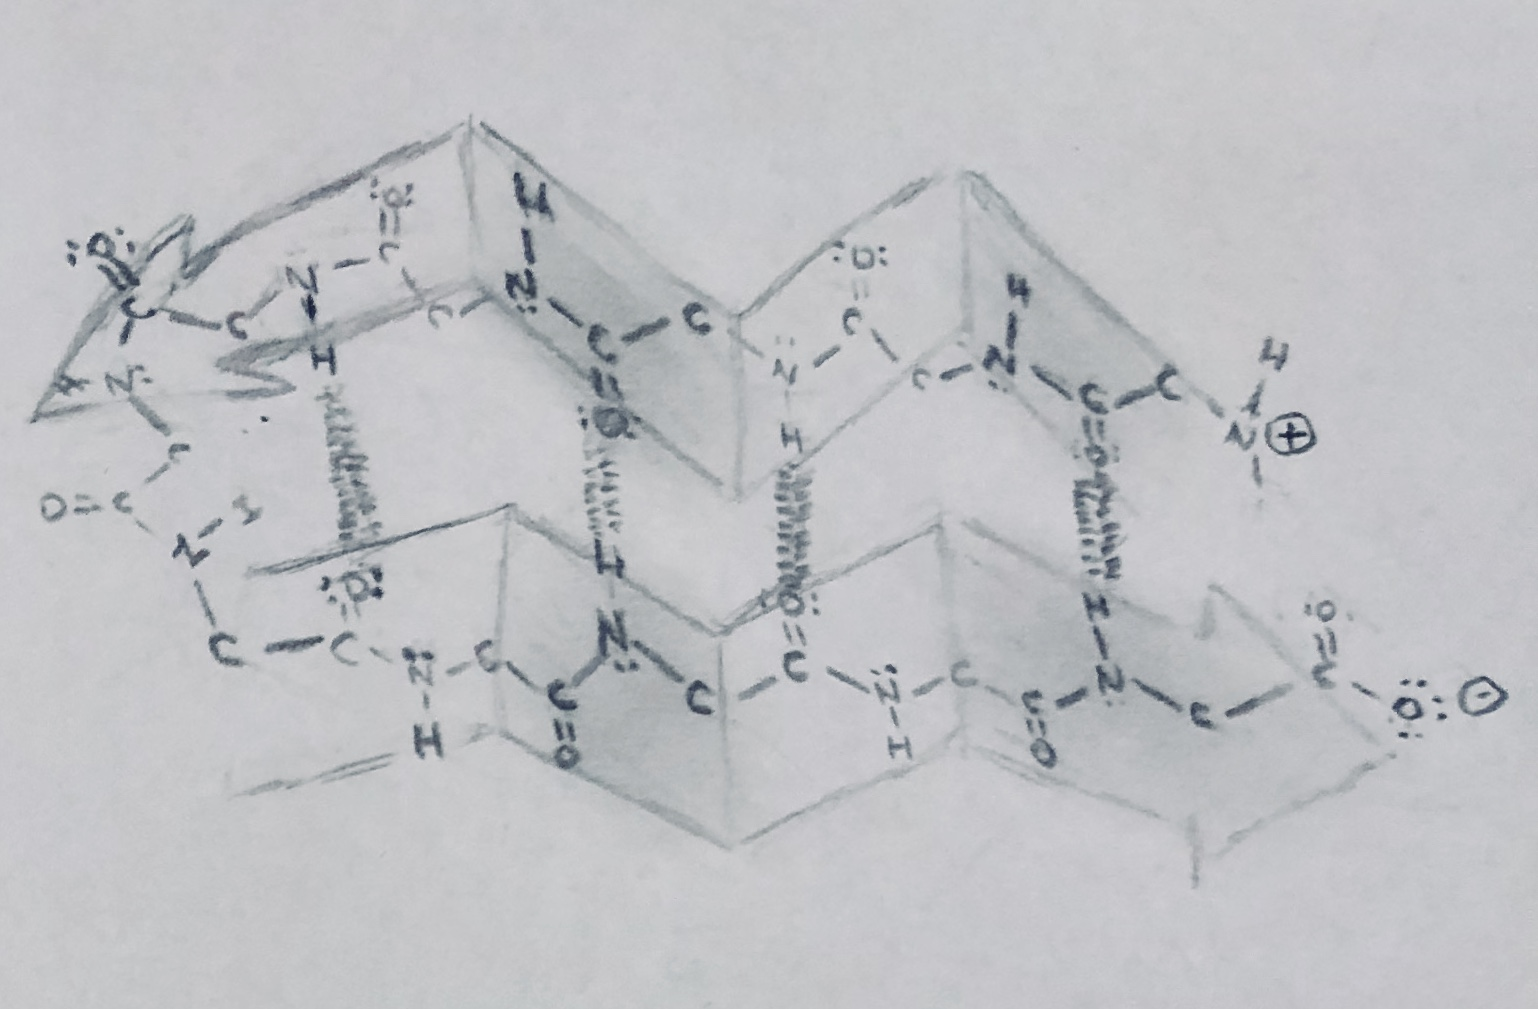
\includegraphics[width=0.8\linewidth]{sheet0.jpg}
    \subcaption{Parallel $\beta$-sheet structure}
    \label{fig:0b}
    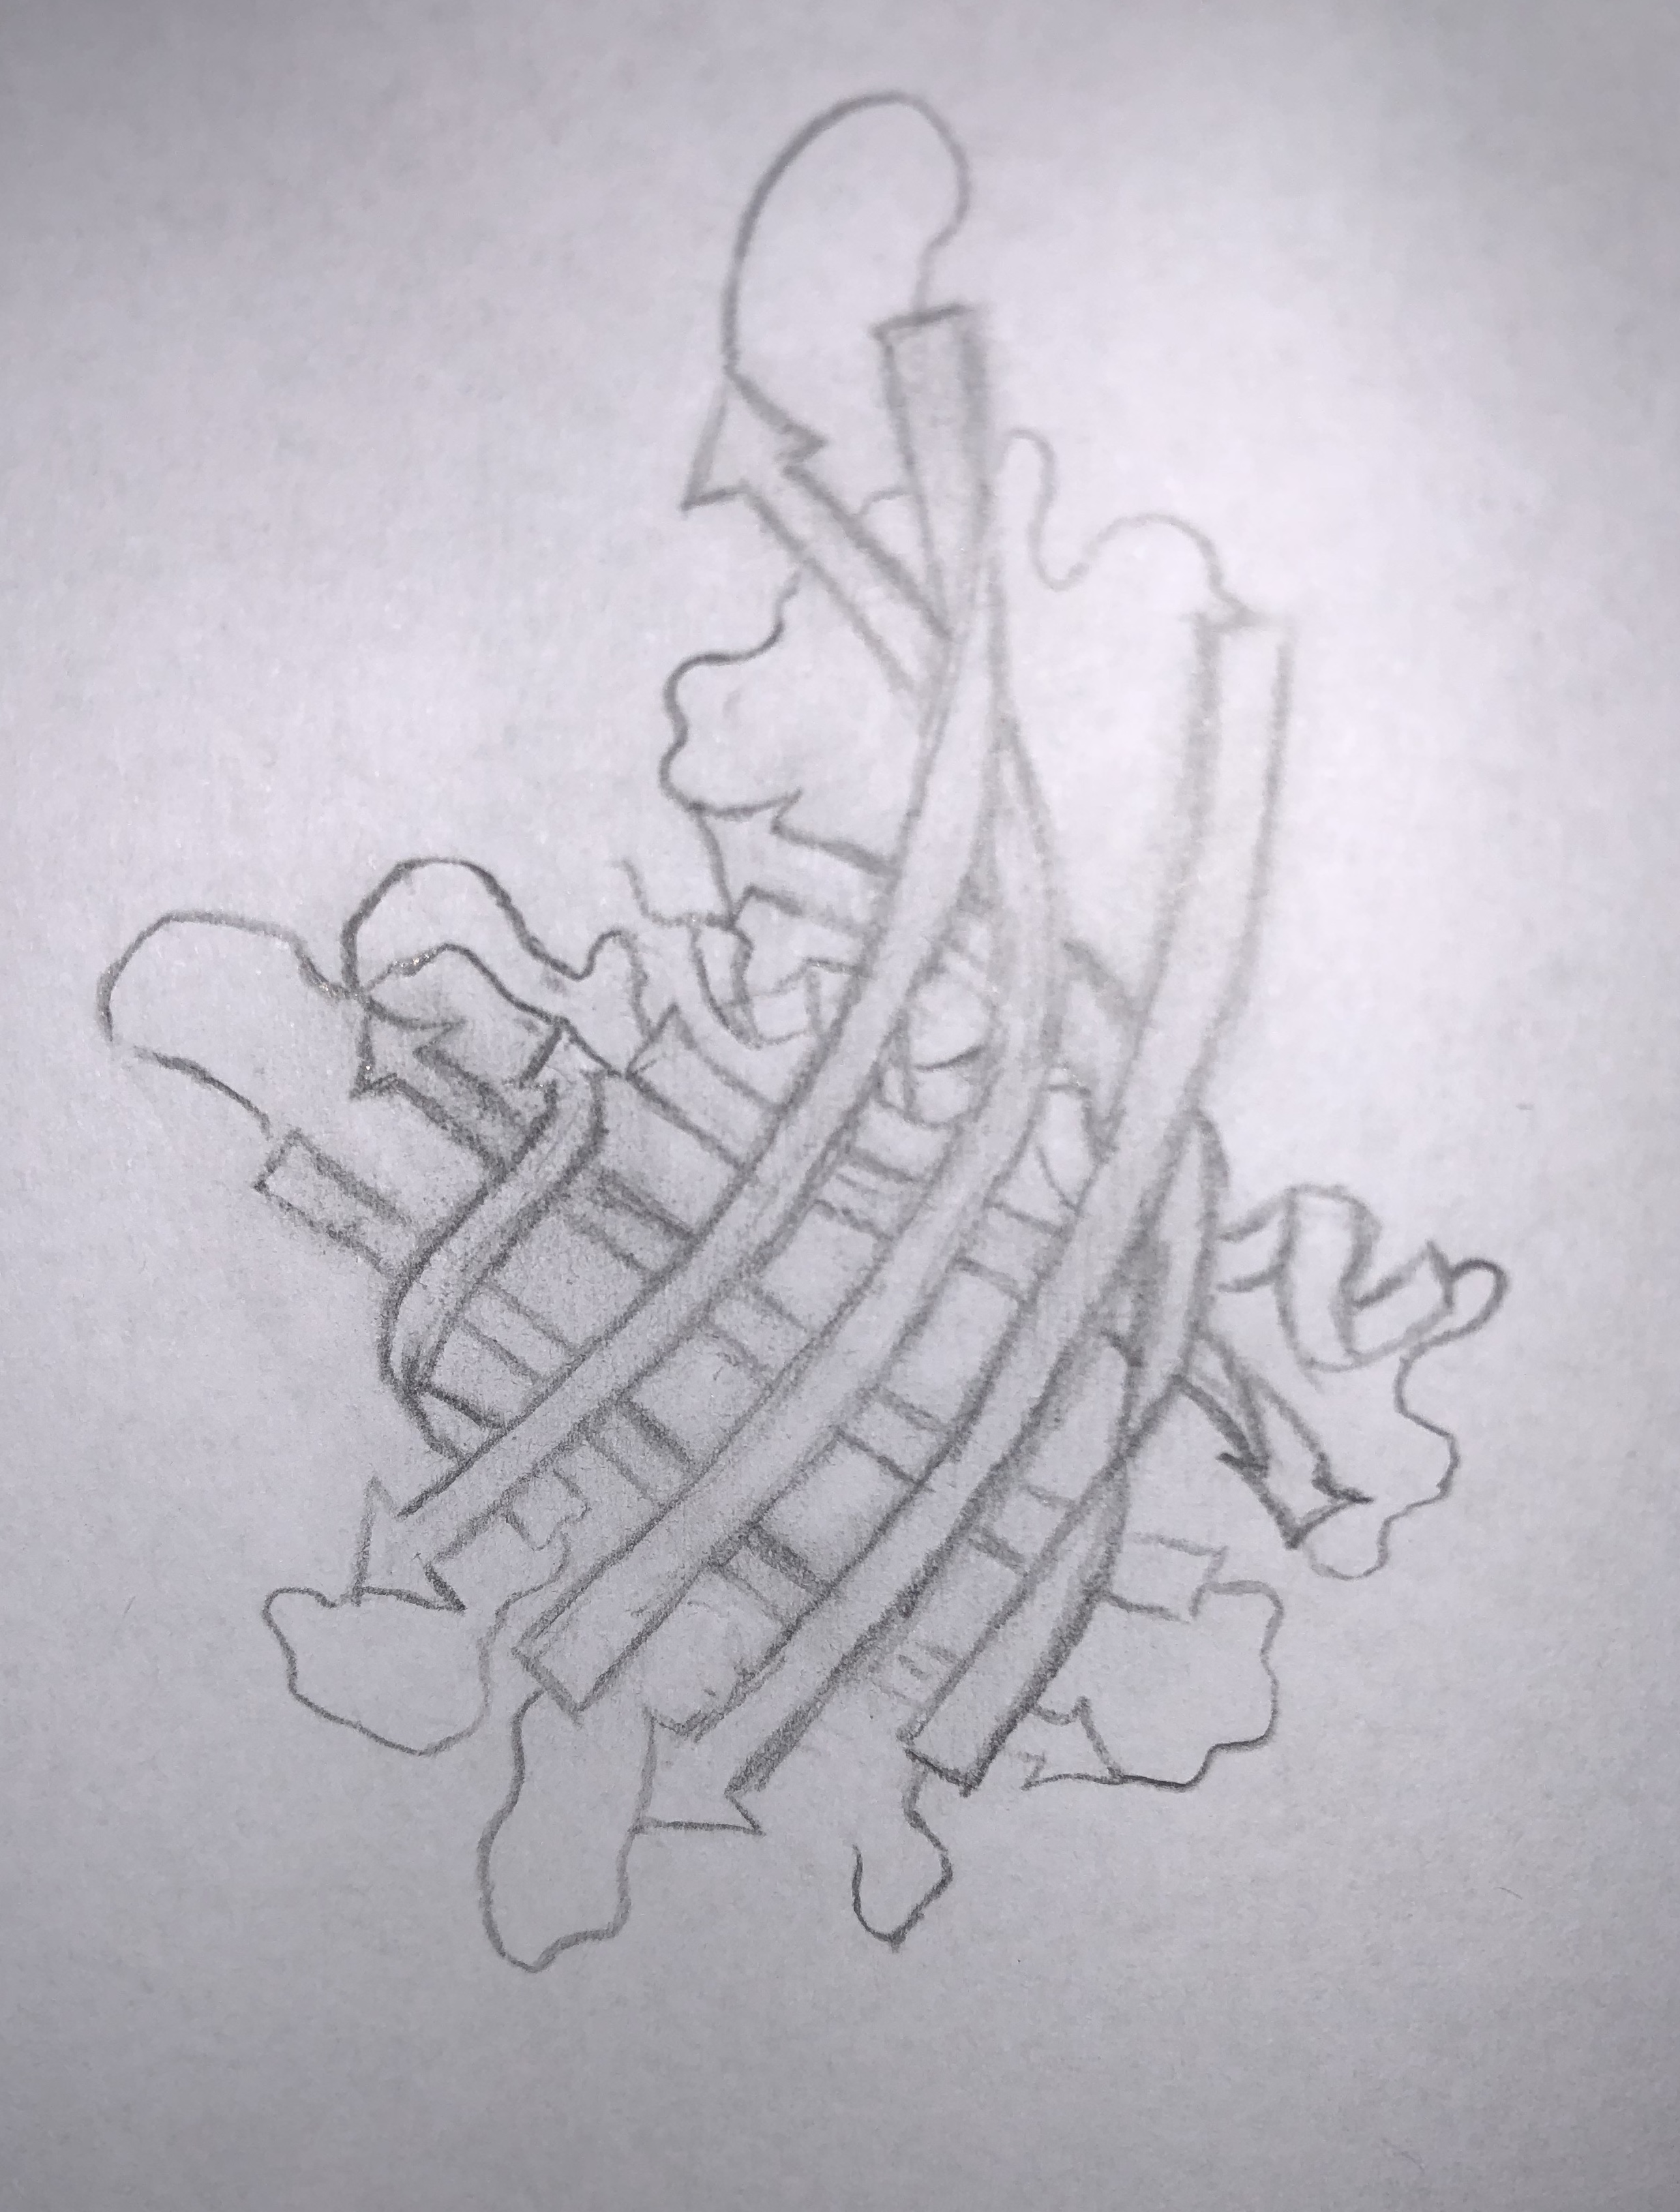
\includegraphics[width=0.65\linewidth]{tertiary0.jpg}
    \subcaption{Tertiary structure of a protein comprised of $\beta$-barrels and an $\alpha$-helix}
    \label{fig:0c}
\end{minipage}
\caption{Levels of protein structure}\label{fig:0}
\end{wrapfigure}
\end{comment}

Firstly, \textit{atoms}, joined by attractive forces called bonds, link together to produce \textit{molecules} called \textit{amino acids} (also known as \textit{residues}). Atoms come in different sizes and shapes but are generally on the order of 1x$10^{-10}$m (1\si{\angstrom}). There are twenty different amino acids, all differing in their side-chain structure and therefore, their physical properties. Each amino acid molecule has a common backbone which begins with a reduced nitrogen atom (amino) and ends with an oxidized carbon atom (acid) with a width of about 4\si{\angstrom}. Some amino acids are polar and charged, interacting with other charged species and water. Others are hydrophobic and "hide from water," through water-exclusion forces. These acid interactions dictate the structure or the "fold" of the protein. Figure 0.2 demonstrates the levels of protein structure: from hydrogen bonding in alpha helices (a) and beta sheets (b), to folds that result in tertiary structure (c).



The structure and dynamics of a protein are determined by its sequence. The amino acid sequence is specified by the genetic code of the organism, known as deoxyribose nucleic acid (DNA). Our DNA is \textit{translated} to messenger ribonucleic acid (mRNA) and \textit{transcribed} to the protein sequence. The linkage of amino acids in a linear "code" is known as the \textit{primary structure} of a protein. When the protein chain lengthens, the protein backbone folds onto itself using non-bonding interactions between the backbone hydrogen and oxygen atoms called hydrogen bonds. These interactions lead to the formation of \textit{secondary structure} like $\alpha$-helices and $\beta$-sheets (see Figure 1a,b). Collections of secondary structural moieties folded on top of one another are the protein's \textit{tertiary structure} (see Figure 1c). Several proteins within the same system are a "complex" and the individual proteins are known as subunits. For example, a protein complex of two regulatory (R) and two catalytic (C) subunits can be written as R$_{2}$C$_{2}$. Two or more subunits within a complex is termed the \textit{quaternary structure} of the protein. Different quantities and arrangements of the same subunits can have different structures and functions. Thus, quaternary structure yields multiplicity in the number of structures a single protein complex can have. 

A slight change in amino acid sequence can alter the \textit{structure} of a protein drastically, and oftentimes, affect its \textit{function}. For example, residues like Glycine (G) confer lots of flexibility in helices, often causing helices to break reversibly. A simple mutation to a more-rigid residue like Proline (P) lead to a physical turn in the structure and this can break a helix without allowing for flexible return the helical moiety. Mutations thus oftentimes affect the way the protein moves and interacts with other molecules, leading to large-scale changes in signaling cascades on the cellular level. Such is true with changes in expression levels of DNA, RNA, proteins, In this way, atomic-level alterations can have a \textit{"biophysical butterfly effect"}, leading to the presentation of disease phenotypes in the organism harboring the mutation. Protein Kinase A (PKA), one of the systems examined by this thesis, is a prime example of a case in which a single-point mutation can alter structure and chemical interactions, and is discussed in more detail below.

\section{How mutations affect protein structure: a multiscale perspective}

Protein Kinase A is found in every multicellular organism. It is responsible for responding to extracellular signals and eliciting an intracellular response; a signal translator and amplifier of sorts. PKA binds a molecule named cyclic adenosine monophosphate (cAMP) in the cyclic-nucleotide binding domain (CBD) regulatory subunit. Once enough cAMP is bound to PKA, the regulatory subunit relieves its inhibition on the catalytic subunit, which is responsible for phosphorylating protein targets, effectively deactivating or activating them in response to an extracellular signal. This tightly controlled mechanism is vital to the function of the cell. Any dysregulation in the response of PKA has major detrimental effects that are common in cancer \cite{Caretta2011}, and endocrine disorders like Carney Complex \cite{Horvath2010}.


There are several isoforms of the Regulatory subunit, denoted by Types I and II and subtypes $\alpha$ and $\beta$. In the RI$\alpha$ isoform, a positively charged reside in PKA, Arginine (R), in position 333 of the regulatory subunit interacts directly with the first molecule of cAMP sensed by PKA. Because of its flexibility, the tetrameric for PKA RI$\alpha$ structure has proven difficult to elucidate \cite{Kim2005}, but scientists figured out that with a mutation of Arginine 333, the dynamics of PKA are stabilized enough for structural biochemists to be able to visualize it using crystallography \cite{Kim2007}.

\setcounter{figure}{2}
\begin{figure}
\centering
	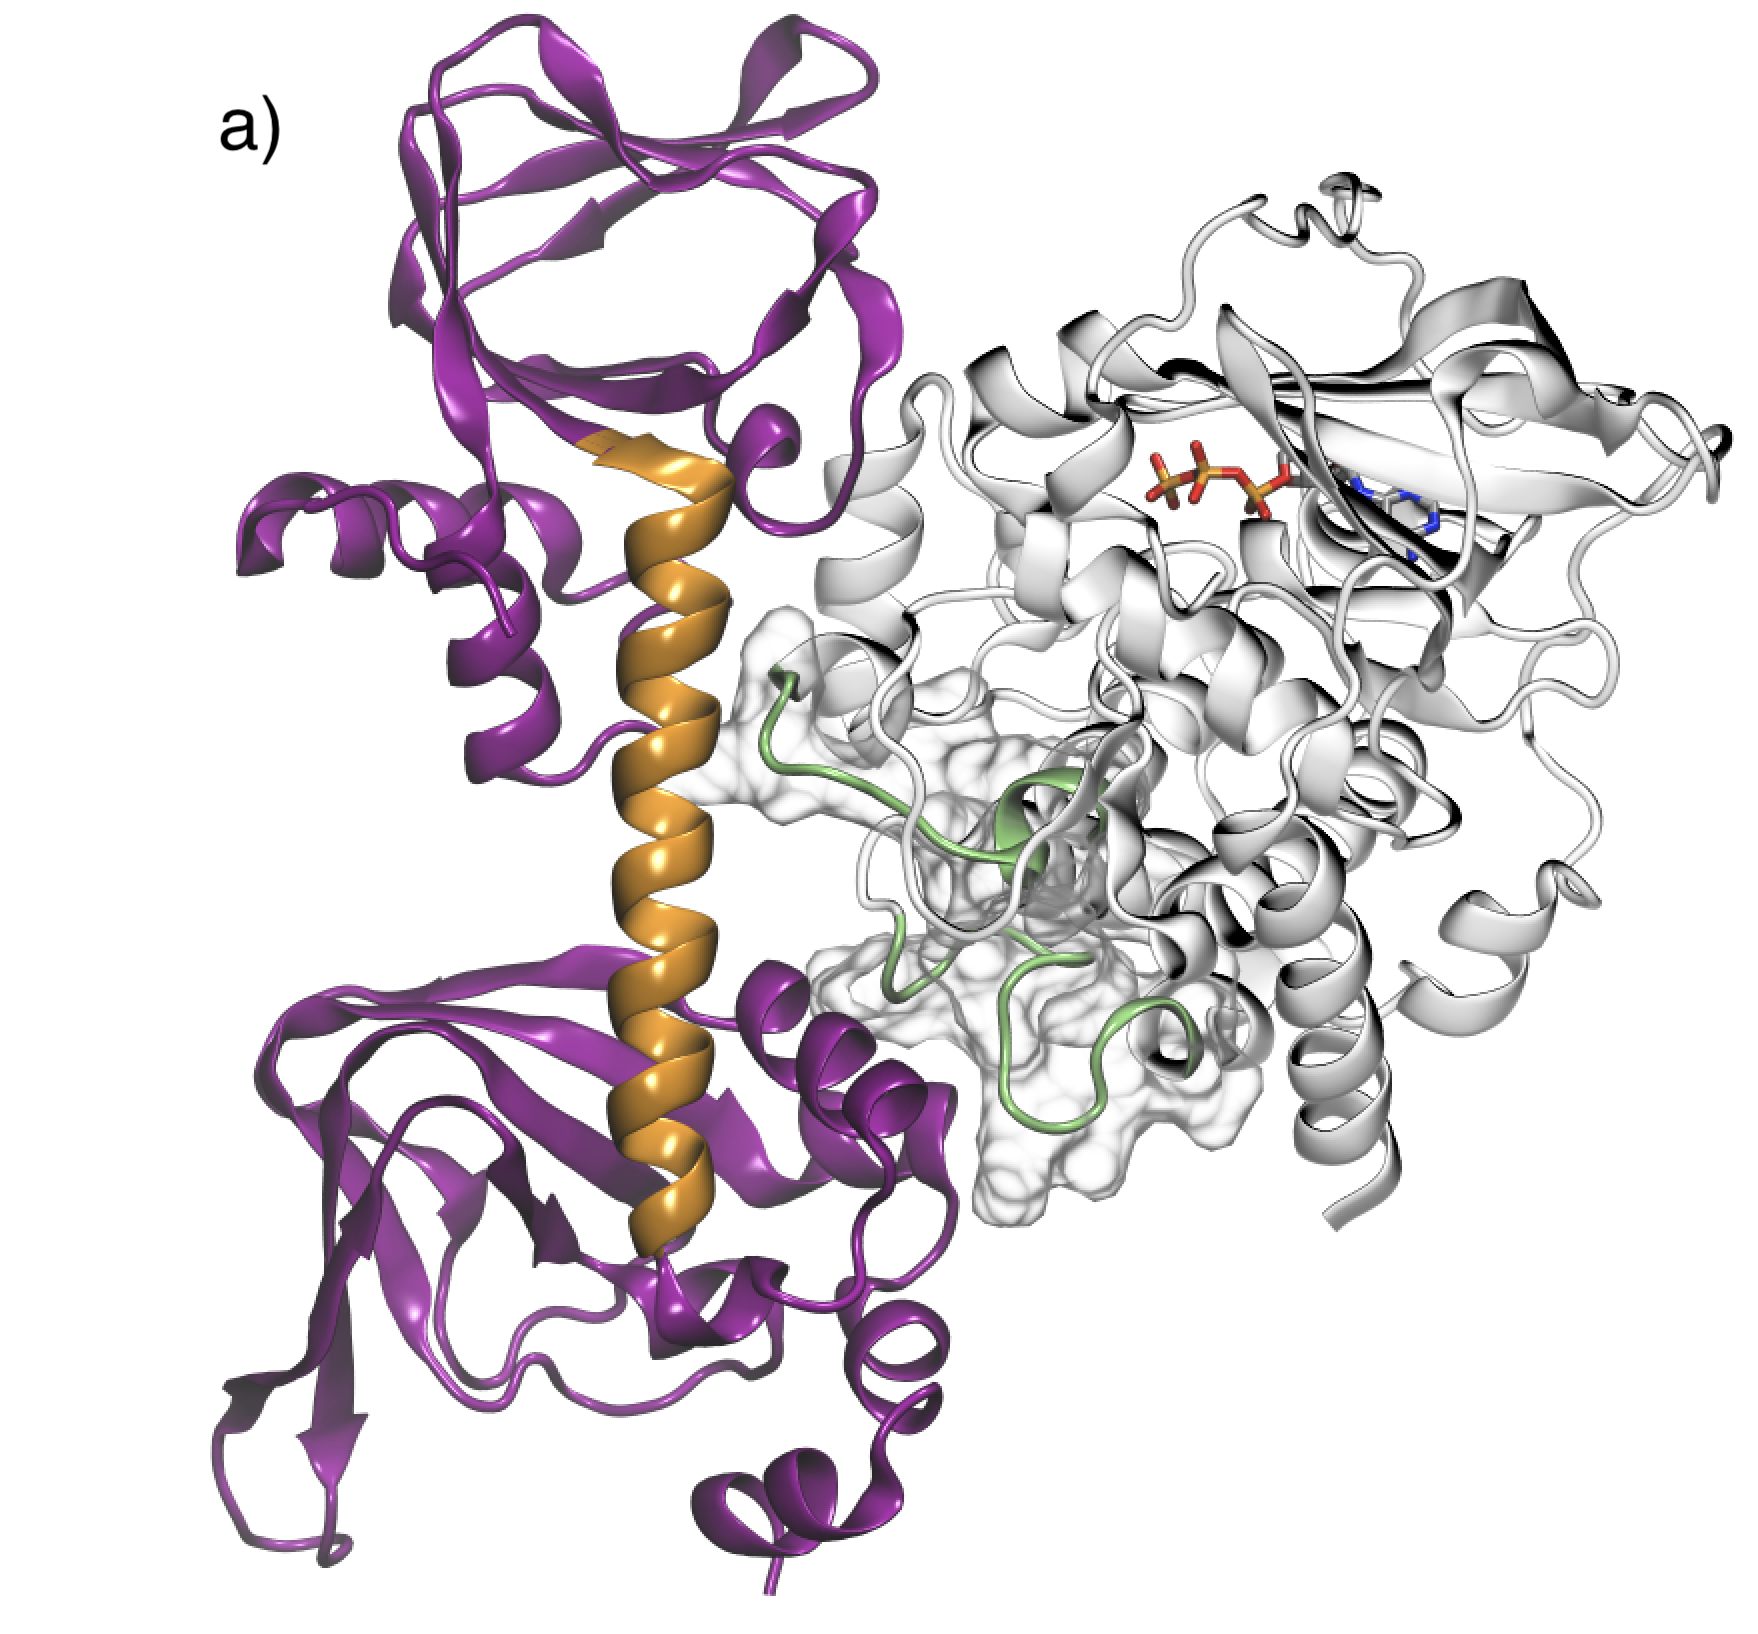
\includegraphics[scale=0.22]{RC_PKA_holo.png}
	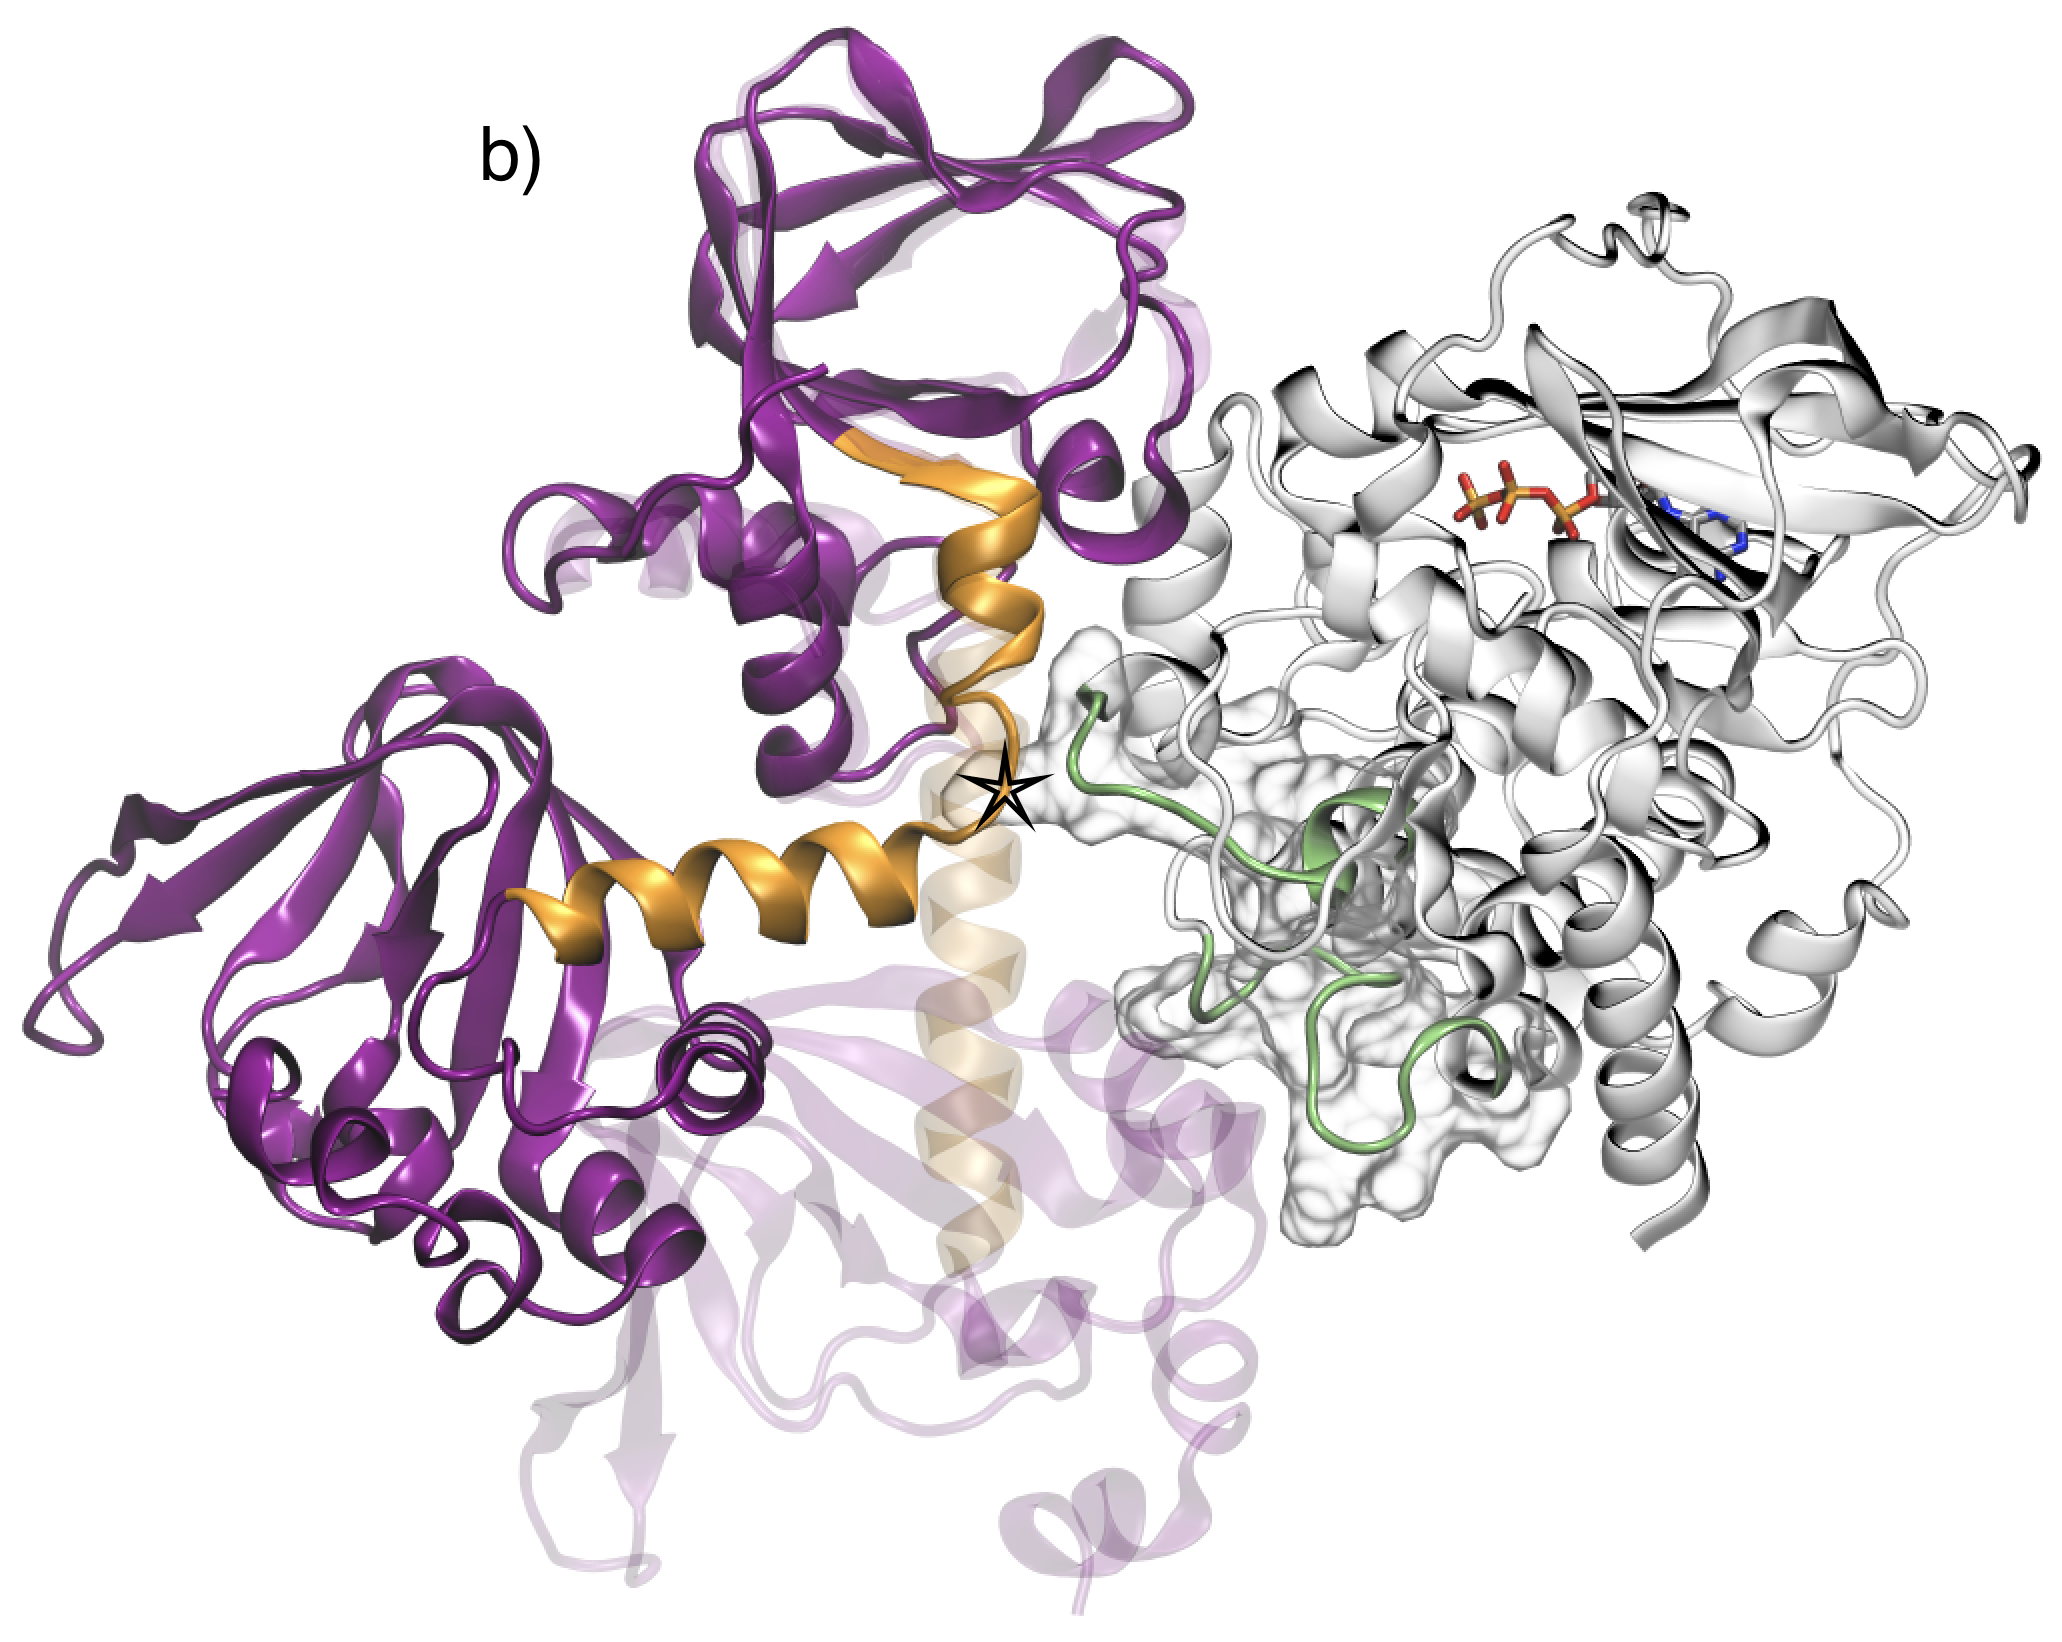
\includegraphics[scale=0.22]{RC_PKA.png}
	\caption{The interface of the Regulatory and Catalytic subunit of Protein Kinase A (PKA), comparing the mutant to the wild-type}
	\subcaption{The mutant Regulatory subunit (R) R333K (purple)  in complex with the Catalytic subunit (C). The B/C helix (gold) connecting the two cyclic nucleotide binding domains (CBDs) is extended in the heterodimeric crystal structure; \textbf{(b)} The wild-type R subunit adopts a stable conformation with a break in the B/C helix at Glycine 235 (black star). The structure is juxtaposed with the R333K mutant (transparent purple) to show the consistency of the WT conformation with the solvent-exposed regions in the C subunit (green) determined by solution experiments}
\label{fig:RC} 
\end{figure}

 When Arginine (R) 333 is mutated to a Lysine (K), which is \textit{also} positively charged, the shape of the PKA molecule changes significantly (see Figure 0.3). This mutation also affects PKA function, altering the way the protein responds to the cAMP signal. In the wild-type (WT) R333 case, the protein is dynamic, with a swinging domain that creates a "butterfly" motion in the protein. It responds to cAMP by dissociating the regulatory subunit from the catalytic subunit, relieving inhibition and activating PKA. In contrast, the K333 mutation makes the protein more globular, neutralizing the motion of swinging domain\cite{Cheng2009} and changes the interaction between cAMP and the regulatory subunit, completely altering the way that PKA is activated. This and other mutations are known to be the root cause of diseases like Carney complex\cite{Kirschner2000} and Adrenocortical Cushing's adenoma\cite{Calebiro2014}. In this way, a single residue mutation effects the dynamics of a protein, and the way that the protein interacts with its environment. 

\section{Structural methodologies for visualization of biology}
As the specialization of this degree is centered on Multiscale Biology, the following chapters will discuss experimental techniques that utilize information gathered from different structure elucidation methods with range in spatial scales from small molecule (\si{\angstrom}), to proteins (nm), to membranous structures on the sub-cellular level ($\mu$m). The following subsections review the pertinent methodologies for biological structure determination and alludes to the ways these methods facilitated scientific investigations in the coming chapters. 

\subsection{X-ray Crystallography}
Crystal x-ray diffraction also known as X-ray Crystallography is popular and widely used method for determining the atomic positions of small molecules and proteins. First developed in 1912 by Max von Laue and later further developed by William Henry Bragg and Sir William Lawrence Bragg \cite{Bragg2014}, crystallography is based on the principal of X-ray diffraction by the atoms in an ordered crystalline substance. 

As the name indicates, the subject of interest is suspended in a crystallographic form and a beam of X-rays at a particular energy, marked by its wavelength, $\lambda$, is shot at the sample. Using the angle, $\theta$ of the diffracted X-ray beams and a mathematical equation known as the Bragg equation: 

\begin{equation}
n\lambda=2d\sin\theta
\end{equation}
Where n is an integer multiple of the wavelength, $\lambda$, d is the distance between the planes of the crystals, and $\theta$ is the scattering angle, one can understand the structure of the biological specimen. From the interference and diffraction pattern produced by the X-ray beam after hitting the crystal lattice structure, one can back-calculate the atomic positions of a molecule. 

X-ray crystal structures yield \si{\angstrom}-level resolution of structure; a real asset for computational chemists and biophysicists who use the atomic positions as inputs for their models. Section 0.5 of the introduction will elaborate more on how atomistic positions are used to understand dynamics and functions of small molecules and proteins. 

It is important to note that an X-ray structure is but a snapshot of a molecule in a single state of its ensemble of conformational states. Although crystal structures are unparalleled in their accuracy of single structure, by their nature, they do not give information about molecular flexibility.  Furthermore, the resolution of atomic positions falls off as molecules increase in size. Therefore, crystallography is limited in the size of the molecules that can be investigated with sufficient accuracy. Fortunately, X-ray structures can be complimented with other structural determination and computational methodologies, which will be discussed in the coming sections. 

Chapter 2 combines X-ray Crystallography with molecular dynamics (discussed in section 0.5.1) in an investigative study of common structural motifs used by an infectious organism. Chapter 3 demonstrates the ways that molecular dynamics can expand on structural information not offered by crystallographic snapshots of proteins. 

\subsection{Hydrogen/Deuterium Exchange Mass Spectrometry}
A remedy for the limited structural states that can be understood with X-ray crystallography is offered by Hydrogen/Deuterium Exchange Mass Spectrometry(H/DxMS).  Since the discovery of the "heavy" hydrogen isotope, deuterium in 1932 by Harold Urey et al. \cite{Urey1932}, deuterium has been used in a myriad of experimental techniques. Early in the 21st century, the application of the deuterium to the study of proteins appeared \cite{Engen2001}. 

As indicated by the name, in H/DxMS, hydrogen and its isotope, deuterium exchange (H/Dx) for one another. This happens specifically with labile hydrogen atoms on the backbone nitrogen of the amino acid, which exchange nearly instantaneously. In a solution of D$_{2}$O (the deuterium version of H$_{2}$O), exchange is rapid if backbone nitrogen are surface-exposed or located in an unstructured region of the protein, and slower if the nitrogen is buried in the core of a protein. Exchange can happen at a rate on the order of milliseconds to seconds if amide nitrogen are not hydrogen bonded, but can take minutes to days if hydrogen bonds are stable. Timescales of exchange translate to the "degree of protection" of the amide, and indicate the degree of flexibility of the structural regions that comprise the protein.The exchange reaction of hydrogen for deuterium is then quenched by acidification of the protein (pH 2.5), which "freezes" the deuteration of the protein. Proteolysis then follows--a method that degrades the protein into smaller fragments to be analyzed by Mass Spectrometry (MS). Mass Spectrometry determines the atomic weight of the fragments, yielding the information of which nitrogen have exchanged their hydrogen for deuterium \cite{Konermann2011}. 

This technique is used to understand the comparative changes in dynamics induced by protein-protein interactions, ligand binding, as well as signaling modes of a protein\cite{Harrison2016}. H/DxMS analysis gives a \textit{dynamic} picture of the protein, allowing biophysicists to understand the flexibility of a molecule. Moreover, the technique is less limited in the size of molecules that can be investigated. 

This method compliments computational methods like Molecular Dynamics which examine the flexibility of proteins. Chapter 3 details how H/DxMS in combination with Molecular Dynamics have brought us closer to a more holistic understanding of the structure of the RI$\alpha$ Protein Kinase A complex, as was briefly discussed earlier. 

While X-ray crystallography and H/DxMS give information about protein structure on the angstrom level, a multitude of methods exist that reveal insights about global structural features of proteins on the nanometer scale.

\subsection{Small-Angle X-ray Scattering}
As discussed earlier, X-ray crystallography utilizes the diffraction, or "bending", of X-rays to resolve the atomic positions comprising molecular structure. But X-rays can also interact with a sample, altering the momentum of the beam in a phenomenon known as \textit{scattering}. In the phenomenon of scattering, the photons in an X-ray beam interact with electrons in a specimen. The scattering pattern indicates the fluctuation of the electron density of the matter being investigated. Put more simply, the scattering profile gives information about the overall shape of a molecule. This is accomplished by measuring the scattering profile in the following way: a photon of wavelength $\lambda$ scatters off the molecular sample at an angle, 2$\theta$, is related to the scattering vector, q through equation 0.2. The intensity of the scattering vector, I(q) is a function of a multitude of factors, including molecular volume, size, electron density. 

\begin{equation}
    q = \frac { 4 \pi \sin ( \theta ) } { \lambda }
\end{equation}

The elegant mathematical theories used to obtain information SAXS experiments are explained best by experts in the literature \cite{Boldon2015}, but to summarize: experimental scattering profile, information such as the molecular weight, molecular volume, and radius of gyration can be determined. What is important to note is that SAXS provides information about an ensemble of structural states, in stark contrast to X-ray Crystallography, which resolve explicit conformations of a molecule. This means that multiple structural states can be "lumped" together in the same SAXS profile if a molecule is flexible. 

 Molecular structure is, by nature, affected by its environment. SAXS has been used to understand molecular structure under particular conditions such as temperature, pH\cite{Carvalho2012}, and in complex with other molecules and proteins\cite{Cheng2009}. Thus, SAXS profile of a protein in its apo or "unbound" state will undoubtedly differ from its profile in a "bound" complex with a small molecule, another protein or even another copy of the same protein (homodimers, homotrimers, etc.)
 
 In the same way, mutations can affect molecular structure resulting in different SAXS profiles when compared to wild-type (WT). Such is the case of a system examined in chapter 3 of this thesis. Using SAXS as a guide, we contextualized the crystallographic structure of PKA combined with the H/DxMS in order to validate the existence of an unresolved conformation of the regulatory subunit obtained by MD, the Flipback conformation.
 
 As is the true with most technologies, crystallography and solution-structure methodologies like H/DxMS and SAXS crystallography have their limitations. That limitation being, molecular size. As the molecular size increases, so often does the difficulty in resolving fine details from the system. As we transcend spatiotemporal scales, we can utilize methods that take advantage of different technologies to gain insight into larger systems. 
 
\subsection{Cryo-electron Microscopy}

Just two years ago, the 2017 Nobel Prize in chemistry was awarded to Jacques Dubochet, Joachim Frank and Richard Henderson for the development of Cryo-electron microscopy (Cryo-EM) in resolving structures of biomolecules in solution. Cryo-EM utilizes an electron beam as an illuminating source to visualize proteins and large molecular species that are flash-frozen in their native structural states. 

Cryo-EM remedies the "single crystalline conformation" limitations of X-ray crystallography and combines the strength of solution structural methods that describe ensembles of structural states, as discussed in the earlier introductory sections. The ingenious method behind Cryo-EM completely avoids the cumbersome crystallization of biomolecules by flash-freezing the subject of study in an aqueous solution. This method, also known as vitrification was developed by James Dubochet along with Jean Lepault nearly 40 years ago \cite{Dubochet1982,Lepault1983,Lepault1986}. The original spray-freezing method evolved further with the use of high-pressure which increases the depth of vitrification \cite{SARTORI1993}. 

Vitrification involves cooling the sample to very low, cryogenic temperatures thus, embedding it a glass-like, irregularly frozen vitreous state upon treatment with liquid ethane. This is a significant advantage over X-ray crystallography, as many proteins will not crystallize easily due to the inherent dynamic nature of proteins in general. It is also especially advantageous for large membrane proteins which are notoriously hard to crystallize.

\setcounter{figure}{3}
\begin{figure}
\centerline{\includegraphics[scale=0.25]{SERCA_RyR.png}}
	\caption{Angstrom-level representations of biomolecules} The Sarco/Endoplasmic Reticulum Calcium-ATPase, SERCA2a, (PDBID:5MPM) crystallized at 3.3\si{\angstrom} resolution (green, left) and the Ryanodine Receptor, RyR2, (PDBID:5GOA) resolved at 4.2\si{\angstrom} with Cryo-EM. 
\end{figure}

Cryo-EM is a popular method for understanding the structure large proteins which can be too "noisy" for solution experiments like H/DxMS and Nuclear Magnetic Resonance\cite{Ishima2000}. In fact, the larger the system, the more intriguing the results of Cryo-EM can be \cite{Frank1995,Lee2015,Sevvana2018}. Figure 0.4 compares the size of SERCA2a, a protein resolved using X-ray crystallography at 3.3\si{\angstrom} (PDBID:5MPM, unpublished) and RyR2, a large (>2MDa) protein at 4.2\si{\angstrom} resolved with Cryo-EM \cite{Peng2016}. The larger the system, the more possible projections of the molecule that can exist. This is because molecules are not oriented when they are captured in vitreous water. Thus, part of the "magic" of Cryo-EM stems from its use in resolving information from randomly oriented molecules. 

Our ability to visualize dynamic, large, and complex Cryo-EM structures is a direct result of Joachim Frank's work in analyzing and processing the images derived from Cryo-EM \cite{Frank1970}. The algorithm, known as cross-correlation, averages ensembles of structural states to resolve what is known as a "single-particle reconstruction" of a biological specimen \cite{Saxton1976}. Using several thousand 2D images of the same molecule in random orientations, the algorithm generates 3D reconstructions from 2D projections\cite{Frank2009}. 
Cryo-EM gives molecular detail on the order of several \si{angstrom}. The size-limitation problem still stands however: the larger the protein, the lower the atomic resolution will be. But the popularity of this method has and will undoubtedly continue to drive the development of both Cryo-EM and the algorithms used to resolve molecular structures. One can only hope that the resolution will improve, yielding atomistic detail. In the context of this thesis, Cryo-EM structures gave us insights into the subcellular context of large structures like the Ryanodine Receptor.  

\subsection{Electron Tomography}
As we scale up from atoms to molecules in living systems, the next "step" is towards the subcellular level. This is realm within which we can see the direct effect of protein function. The name, "subcellular," alludes to the fact that this scale is a part of a cell. At this level, organelles-- boundaries that distinguish specialized regions of the cell--become the subject of focus. To see within the cell, we can use a special technique used to determine the 3D structure of a cell known as electron tomography. 

As its name indicates, electron tomography uses an electron beam as its source of a penetrating wave of energy. Tomography is an imaging technique that "sections" or penetrates the object being visualized. In the case of electron tomography, a biological specimen undergoes a tilt-series, where the sample is exposed to the beam at different angles resulting in different projections of the specimen \cite{Fridman2012,Koning2018}. The specimen itself is fixed with chemicals that "lock-in" the physical structure and stained with heavy metals that increase the contrast of lipids and proteins. Gold particles are used as fiduciary markers to align projections. Upon alignment, the boundaries of important structures are traced and used for reconstruction on the sub-volumes \cite{Yu2008,Lee2018}.

Three-dimensional reconstructions of subcellular volumes are used in this thesis to understand the dynamics of calcium signaling in cardiac tissue\cite{Hayashi2009} as first pioneered by Hake et al \cite{Hake2012}. In the fourth chapter these realistic geometries are used as a framework within which we reconstitute the biochemical reactions that underlie calcium signaling. Additional details will follow in the final section of the introduction and in chapter 4 of the dissertation. 

\section{Biophysical structure modeling methodologies}
Studying the dynamics of biological systems is no simple feat. Proteins are incredibly small and their relevant motions are fast; oftentimes too fast to study with available technology. Fortunately, a number of computational tools that simulate molecular motion exist. This section contains a brief introduction to two such computational tools used to model the dynamics of proteins, Molecular Dynamics and Brownian Dynamics. 

\subsection{Molecular Dynamics}
Since the late 70's, computers have been used in the field of biochemistry, providing visual insights into dynamics of proteins\cite{Levitt1975,McCammon1979}. Since the first simulations of bovine pancreatic trypsin inhibitor, the field of biomolecular simulation has expanded both in the systems that have been investigated, along with the algorithms used to compute the forces that govern molecular motion.

Molecular Dynamics (MD) is a computational technique used to compute the spatial and temporal atomic motions according to Newton's equations of motion, where \textit{F} is force, \textit{m} is mass, and \textit{a} is acceleration (see equation 0.3). The gradient of potential energy, \textit{U} in space is described by equation 0.4 where $\vec { R }$ are the coordinates of all of the atoms in the structure. These atomic positions oftentimes are often determined by X-ray crystal structures as discussed in earlier sections.

\begin{equation}
   F = ma
\end{equation}

\begin{equation}
   F ( \vec { R } ) = - \nabla U ( \vec { R } )
\end{equation}

For a large system, the analytic solution of this function is impossible to solve, but a numerical solution is made possible using a collection of equations that describe the forces that influence atomic motions. Time is discretized, or subdivided into small steps. In MD, simulated time is on the order of 1 to 2 femtoseconds (fs), $1\times10^{-15}$ s. After every time step, we solve for the potential energy function by adding the forces acting on every atom in the system. The forces can be split into bonding and non-bonding forces as they are in equation 5, below.  

\begin{align}
  \label{eq:eight}
   \begin{split}
    \begin{gathered}
     U ( \vec { R } ) = \underbrace { \sum _ {bonds} k _ { i } ^ \text {bond} \left( r _ { i } - r _ { 0 } \right) ^ { 2 } +  \sum _ { angles } k _ { i } ^ { \text { angle} } \left( \theta _ { i } - \theta _ { 0 } \right) ^ { 2 } }_{ U _ {\text{bonding}} }\\ \underbrace { + \sum _ { {dihedrals} } k _ { i } ^ {\text{dihe}} \left[ 1 + \cos \left( n _ { i } \phi _ { i } + \delta _ { i } \right) \right]   +  \sum _ {improper} k _ { i } ^ { \text {impr} } \left( \varphi - \varphi _ { 0 } \right) ^ { 2 }   }_{ U _ {\text{bonding}} }\\
     + \underbrace{ \sum _ { i } \sum _ { j \neq i } 4 \epsilon _ { i j } \left[ \left( \frac { A _ { i j } } { r _ { i j } } \right) ^ { 12 } - \left( \frac { B _ { i j } } { r _ { i j } } \right) ^ { 6 } \right]
      + \sum _ { i } \sum _ { j \neq i } \left(\frac {q _ { i } q _ { j } } { \epsilon r _ { i j } }\right)} _ { U _ { \text{non-bonding}}}
    \end{gathered}
  \end{split}
\end{align}


The bonding potential term is defined as the oscillation of the equilibrium bond length. The angular potential is defined as the oscillation of three atoms forming an angle. The dihedral potential is a torsional relation of four atoms oscillating about a central bonding axis. The improper dihedral potential is defined as the the torsional relation of three atoms connected to a single common atom. All bonded forces are described by corresponding spring constants (${k}_{i}$) with radial distances (\textit{r}), angular ($\theta$), proper dihedral angle ($\phi$), and improper dihedral angle ($\varphi$)  terms. These terms have an initial value and value after every time step (0 and \textit{i}, respectively). 

The van der Waals potential, which is synonymous with the total intermolecular forces, is expressed as a "6-12" Lennard Jones potential, or the difference between experimentally determined values Aij and Bij over the radial distances, r$_{ij}$ multiplied by the Lennard Jones well depth, $\epsilon_{i}$. Finally, the electrostatic potential, the effective attraction and repulsion of charged or partially charged atoms, is proportional to the partial atomic charges of the atoms (q$_{i}$ q$_{j}$), and inversely proportional to the interatomic distances (Rij). 

The summation of the bonding and non-bonding forces over iterative timesteps yields a spatial displacement of each atom in the system. Collectively, is results in the motion of the atoms in the system, or \textit{intramolecular motion}. Iterative solutions of these equations through time result in a trajectory of atomic motion. This is, effectively, a change in structure as a function of time, where the protein moves and responds to its environment. The amount of linear time that can be simulated depends both on the size of the protein (in number of atoms) and amount of computational power available. The larger the system, the more computational power required and the longer it will take to compute the dynamics. Today, it is routine to simulate nanosecond-microseconds of time with MD, though there are methods that can access millisecond timescales and beyond\cite{Shaw2009,Pierce2012}. 

The energetic terms associated with each atom in a system are collectively called a molecular mechanics "force field." Depending on what the user is modeling-- lipids, carbohydrates, nucleotides, proteins, metals--one can find force fields specialized in the accurate prediction of the dynamics of the chosen system. Some examples of force fields are AMBER\cite{CaseD.A.BetzR.M.CeruttiD.S.CheathamT.E.IIIDardenT.A.DukeR.E.GieseT.J.GohlkeH.GoetzA.W.HomeyerN.IzadiS.JanowskiP.KausJ.KovalenkoA.LeeT.S.LeGrandS.LiP.LuchkoT.LuoR.MadejB.MerzK.M.MonardG.2015}, CHARMM \cite{Brooks2009}, GROMACS \cite{VanDerSpoel2005}, and OPLS \cite{Damm1997}. The forcefields are used to design the system in terms of energetics, and the potential energy function is calculated with a molecular mechanics engine. The engines have been developed with their own force fields such as the GROMOS MD engine \cite{Christen2005} that is used with the GROMACS force field. Some popular molecular mechanics engines include AMBER \cite{Pearlman1995}, NAMD \cite{Nelson1996}, GROMOS \cite{Christen2005}, and Desmond \cite{Bowers2006}. Many force fields and engines can be mixed-and-matched, leaving the decision up to the user on what combination best suits their study.

The protein being investigated using MD can represent the solvent in one of two ways: explicitly or as a continuum. The explicit solvent description models models every atom in the solvent including ions and water; sometimes even dummy atoms that are meant to model the behavior of the electrons in the molecules. In the continuum approach, the solvent is modeled inexplicitly as an electric field. The latter approach yields increased computational power as water calculations take up significant amounts of time and computational resources \cite{Anandakrishnan2015}. Nevertheless, water interactions with the system are oftentimes important, so there is an information trade-off for inexplicit water modeling. Additionally, there are a wide variety of explicit water models that can be used to simulate a chosen system \cite{Florova2010}. 

MD has a long, successful track record of uncovering the hidden features of protein motions \cite{Hospital2015}. In these cases, that which is not revealed by crystallography or other structure determination techniques can be further understood with the use of molecular dynamics. In this thesis, MD will be applied to the intramolecular investigations of several systems. The first chapter highlights ways that molecular dynamics simulations can yield an understanding of the kinetic transitions as well as provide new structural states to be interrogated by intermolecular investigation methods. Molecular dynamics is then used to understand the effects of mutations in a protein-protein system in chapter 2. Finally, in chapter 3, MD is used to elucidate a conformation of PKA that has been elusive to crystallographers.

\subsection{Brownian Dynamics}
As we scale upwards through biomolecular space and time, the next level we reach centers on the \textit{intermolecular} interactions \textit{between} molecules.Brownian Dynamics (BD) is a method developed to model bimolecular diffusion that estimates kinetic association events. This is especially useful for the step-wise understanding of complex biochemical mechanisms. 

BD is specifically focused on the determination of second-order association kinetics between proteins and their binding partners, be they proteins, small molecules, or ions. BD uses several main assumptions in order to accomplish this. Firstly the solvent is modeled using a dielectric field and ionic continuum. In stark contrast to MD, most often, BD models the atoms in a molecule as rigid bodies. Furthermore, each atom is modeled as a hard-sphere and the atomic forces include mostly electrostatic forces. 

\setcounter{figure}{3}
\begin{figure}
\centerline{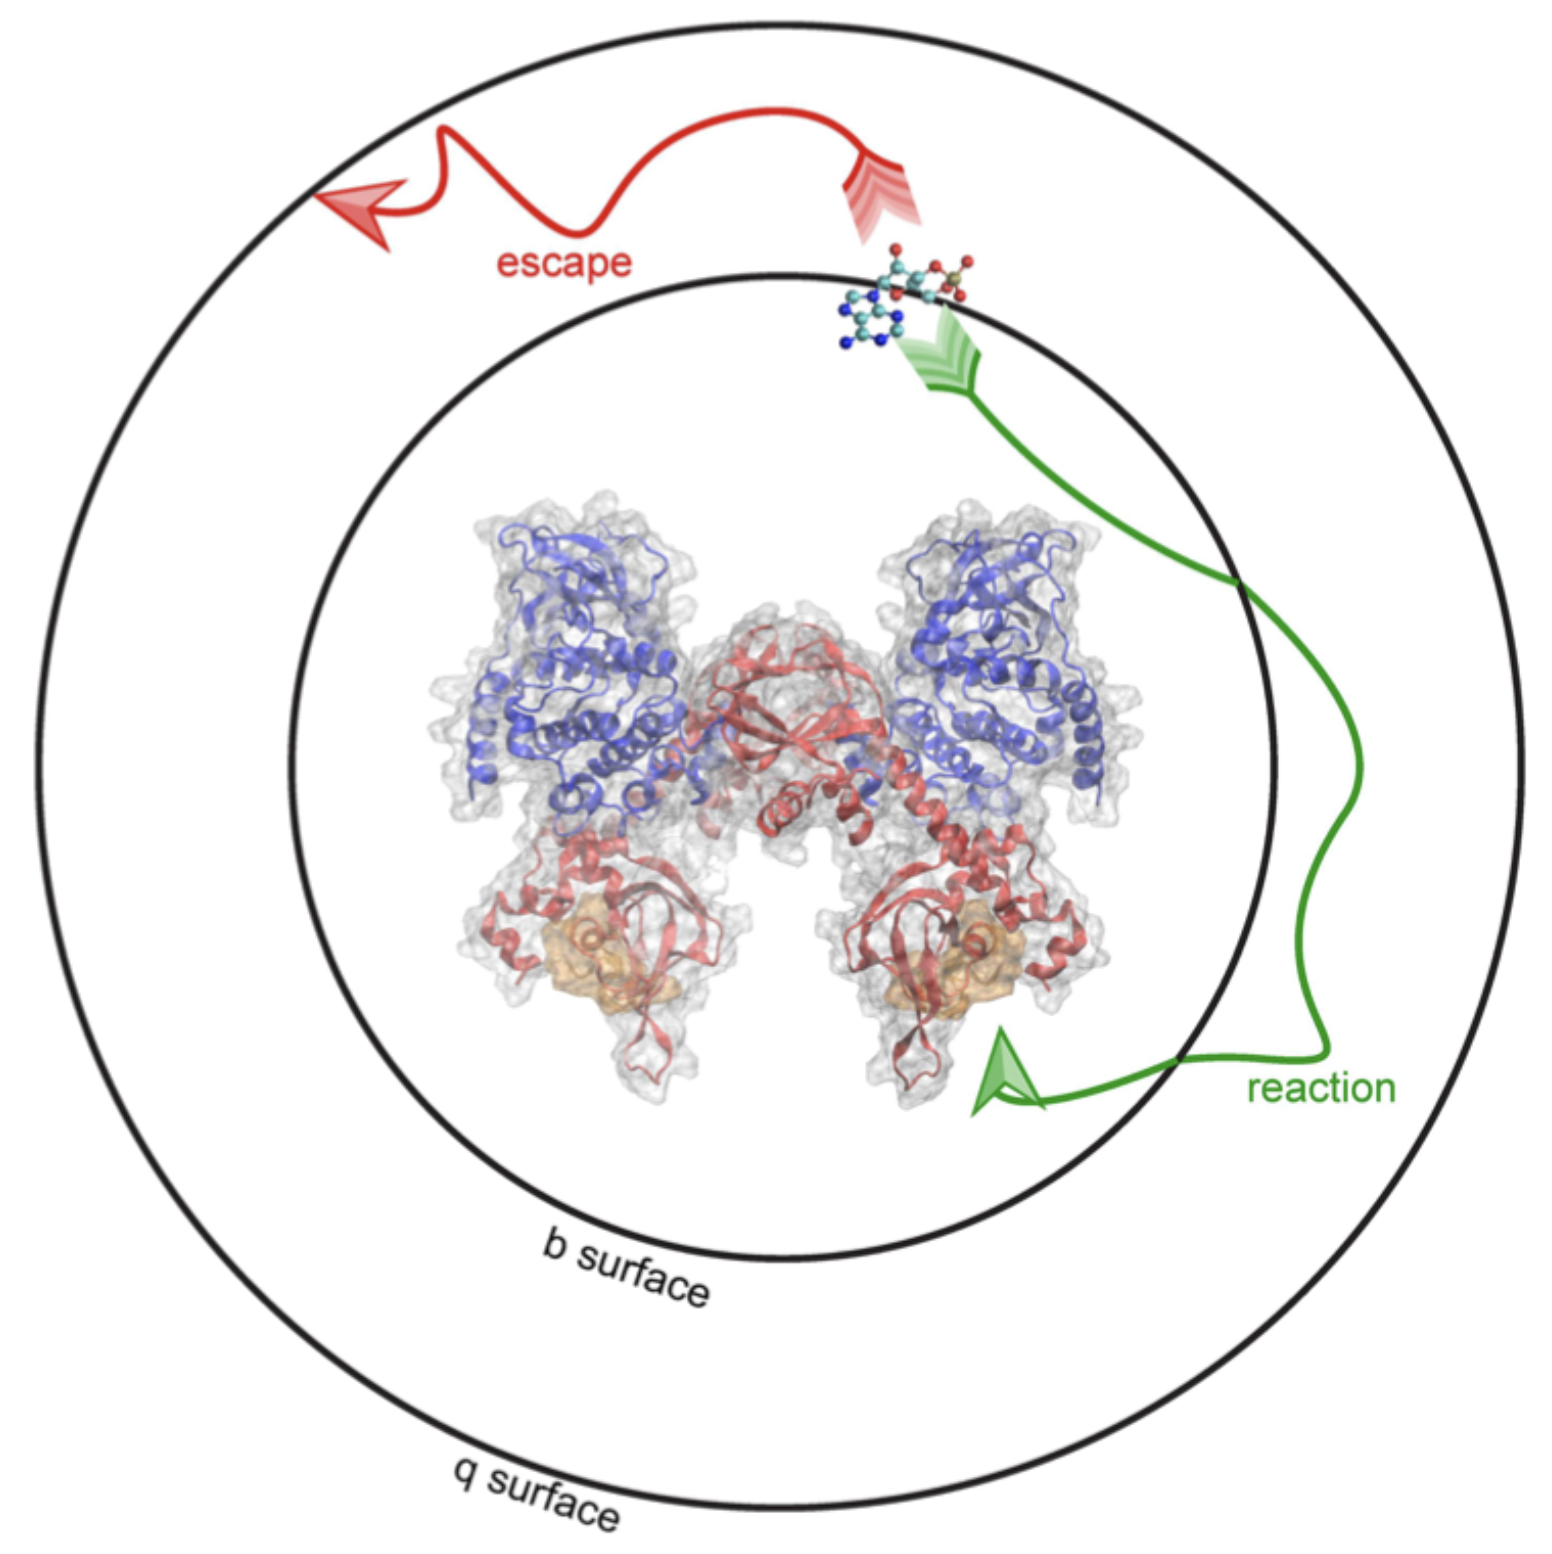
\includegraphics[scale=0.3]{BD.png}}
	\caption{Brownian Dynamics simulation with BrownDye} A molecule begins on the centrosymmetric b-surface and can either escape (red arrow) beyond the q-surface or associate (green arrow) to the specified binding region (gold)
\end{figure}

The equation of molecular motion (equation 0.6) in a BD is a function of the position (x), rotation ($\phi$), attractive and repulsive forces (F), and the torque (T) of a particle index (i). A random vector (w) simulates the random "kicks" of water on the diffusion of the particle, an effective "Brownian motion" factor. D is the diffusion tensor and s the matrix square root of the diffusion tensor \cite{Huber2010}. 

\begin{equation}
    d \left( \begin{array} { c } { x _ { i } } \\ { \varphi _ { i } } \end{array} \right) = \frac { d t } { k _ { B } T } \mathbf { D } \cdot \left( \mathbf { T } _ { i } \right) + \sqrt { 2 d t } \mathbf { s } \cdot w + \nabla \cdot \mathbf { D } d t
\end{equation}

The algorithm used to compute rate constants from the Brownian trajectories was developed by Northrup, Allison and McCammon \cite{Northrup1984} and is known in the field as the NAM algorithm. Using the NAM algorithm, one can determine the spatial trajectory of diffusing molecules in 3D space. A number of BD simulation programs exist, including SDA \cite{Gabdoulline1997,Gabdoulline1998}, ReaDDy \cite{Schoneberg2013}, Brownmove \cite{Geyer2011}, \texttt{BD\_BOX} \cite{Dugosz2011}, and BrownDye \cite{Huber2010}. In order to set up a simulation, one must parameterize system by assigning the appropriate parameters to each atom. The relevant terms in the case of BD are van der Waals radial (r) and charge (q) values that are assigned using MD force fields like the ones discussed in  section 0.5.1, earlier. Using the charge and radial parameters, an electrostatic description of the molecule in the form of a charge field can be calculated using programs like DelPhi \cite{Honig1995} and APBS \cite{Baker2001}. In this thesis, the program BrownDye is used to perform BD simulations and APBS is used for the electrostatic description of the biomolecules. 

In BD simulations with BrownDye, diffusing molecules are placed at a radial distance \textit{b} from oneanother. The simulation begins by placing the diffusing molecules at different distances of b distributed over a spherical surface, called the "b-surface" (see figure 0.4). Molecular diffusion begins at the start of the simulation and ends in one of two ways: 1) diffusion past a certain distance "q" or the "q-surface"; or 2) with association of the two molecules after satisfying the contacts set by the user in the encounter complex description \cite{Huber2010}. The timescale of integration is typically on the order of picoseconds (1 $\times$ 10$^{-12}s$). With the speed of BrownDye, millions of trials can be run on a desktop computer to estimate $\beta$, or the probability that a binding partner located on the b-surface will satisfy the encounter complex and "react" rather than escape beyond the q-surface. Figure 0.5 demonstrates the basic principles of the BrownDye simulation package used to determine the rate constant of bimolecular association, k$_{on}$ (see equation 0.7, below).

\begin{equation}
    \boldsymbol { k } _ { o n } = \boldsymbol { k } _ { b } \boldsymbol { \beta }
\end{equation}

The rate of diffusion of the ligand to the b-surface, k$_{b}$ can be calculated using equation 0.8, below. k$_{b}$ is a function of  U(r), the effective potential energy at a distance r from the center of the sphere, the temperature, T, Boltzmann's constant, k$_{b}$, and the diffusion coefficient, D, which varies with radial distance, (r).

\begin{equation}
    \boldsymbol { k } _ { b } = \frac{ 4 \pi} { \left[ \int _ { \mathbf { b } } ^ { \infty } \frac { \exp \left( \text { U } ( \boldsymbol { r } ) / \boldsymbol { k } _ { B } \boldsymbol { T } \right) } { \boldsymbol { r } ^ { 2 } \boldsymbol { D } ( \boldsymbol { r } ) } \boldsymbol { d } r \right] }
\end{equation}

Models of the structural and kinetic properties of biomolecules are useful not only to those experimentalists seeking to further understand and visualize the behavior of biochemical systems, but also to computational biologists seeking to model biochemical phenomena on the cellular level. Using BD simulations, we can tease out the association rates between to molecules which is often difficult to measure with experiments. Chapter 1 will demonstrate the ways in which this kinetic information can be used in higher-order cellular models. In chapter 3, Brownian Dynamics will be applied to the understanding of cAMP association to PKA.  

\section{Subcellular biochemical modeling methodologies}
As we continue transcending through the scales of space and time, having already explored intramolecular and intermolecular biophysical methods, we arrive at the scales within which these biochemical properties exert their effects: the subcellular level. Even the slightest alterations in chemical structure and function can have dramatic effect on the dynamics of cellular systems; what I like to call "a biophysical butterfly effect." Biological modeling at this level allows for the holistic understanding of the biochemistry within the subcellular space. This is especially useful for complex systems where multiple competing reactions occur. More specifically, it is useful for the comparison and contextualization of reactions in biological systems. A number of methods that model diffusion and reactions on the molecular level have been developed and used extensively to explain and predict biological observables. %The following important distinctions between computational biology modeling methods will be described: 1) deterministic vs. stochastic; 2) network vs. rule-based ; 3) non-spatial vs. spatial; and finally, 4) population vs.agent-based, also known as continuum vs discrete. Alternatively, partial differential equations (PDE), which are functions of multiple variables, can be used.


\subsection{Modeling biology with differential equations}
Biochemical descriptions of biological systems are almost always complex. In a given cell, anywhere from hundreds to thousands of different molecular species exist. The reactions between these species only intensifies the complexity when you consider that these molecules react with many different partners to create more molecules. Yet again, mathematics comes to the rescue, giving biologists, chemists, and physicists a language that can be used to model biological systems. One can describe the dynamical system in terms of the change in molecular concentration and local density with respect to time. 

Modeling the change of a single feature of a molecular system, say a given concentration, with respect to time, is the essence of an Ordinary Differential Equation (ODE). Reactions, too, can be described in this way, where the concentrations of molecular species change as a function of the forward and reverse rate of consumption. Molecular diffusion in single and multiple can also be modeled with ODEs making this a powerful method for understanding the temporal evolution of gradients in cellular systems \cite{Faeder2009}.

One can also model the change in a system as a function of several simultaneously changing parameters. Consider for example, modeling the rate of change as a function of time through a particular three-dimensional region, like an organelle. This is arguably a more complex problem As it involves a \textit{spatial description} of the system. To model systems like this, one could use spatial ODE solvers \cite{Harrison2016} which use specialized algorithms to model diffusion through space. Partial differential Equations (PDEs) can also be used for this purpose but are comparatively more computationally intensive to solve as space has to be subdivided into elements within which diffusion is computed. What is common to modeling with differential equations is a very important factor: the continuum assumption.

The fundamental component of all differential equations in biological simulation methods is the use of non-discrete representations of molecular species, or a continuum. That is, all the elements of a species are non-distinguishable from one-another. In ODE and PDE biological simulations, molecular concentrations are modeled as a "field" that evolves in its intensity with the passage of time according to the equations that describe its temporal evolution. This approximation works well for large molecular quantities that are well-mixed. It falls short, however, when we consider situations in which chemical concentrations are extremely low.

\begin{comment}
One would agree that biology has a \textit{hint} of unpredictability or randomness to it; especially when it comes to the movement of small molecules in large, complex sub-volumes. Therefore, it is appropriate to use stochastic methods for modeling subcellular dynamics. Stochastic differential equations can be used in these cases
\end{comment}


\subsection{Discrete subcellular spatial modeling}
As insinuated in the earlier section, there are delicate systems in biology where molecular concentrations are extremely low. For example, a region in the cardiac muscle cell that sits between the plasma membrane and an organelle named the sarcoplasmic reticulum (SR), the dyadic cleft, has a range of zero to three molecules in the subspace at equilibrium\cite{Bers2002}. In such cases, it is inappropriate to treat molecules as a continuum. Instead, we can model the molecules discretely using algorithms that track the spatial location of these ions. The more we seek to model realistic phenomena in biology, the more we need to consider the importance of stochasticity and explicit spatial encounters in biological systems. Using the program MCell \cite{Stiles2001a,Kerr2008}, we can accomplish exactly this. 

MCell is a Monte-Carlo is a simulation method that stochastically and explicitly models the 3D diffusion and reaction of molecular species by treating them as particles. The Monte-Carlo technique uses random number generator that "chooses" from an ensemble of values which correspond to the spatial displacement of molecules in the system. In the context of subcellular modeling, Monte Carlo algorithms are are aimed at representing the stochastic nature of a biochemical system. The algorithm describing motion in MCell is a simplified, unbiased random walk. Molecules are modeled as volume-less points that diffuse according to assigned diffusion parameters. 

One of MCell's most impressive attribute is that it is a \textit{master counter}. At every integration timestep, often on the scale of microseconds ($1 \times 10^{-6}s$) molecules have the potential to either react, diffuse, or remain unchanged. MCell explicitly counts not only the number of particles but tracks their spatial location in subcellular geometries. Molecular reactions can be unimolecular or, upon spatial encounter of two species, bimolecular. Reactions can happen with two freely diffusing "volume" molecules, or between membrane-bound "surface" molecules and volume molecules. Surface molecules are also capable of 3D diffusion and changing their orientation in a membrane. 

Using mesh generation tools like GaMer \cite{Yu2008, Lee2018}, cellular reconstructions obtained from electron microscopy can be reconstructed into usable meshes for biological simulation. These complex subcellular geometries can be imported into CellBlender \cite{Gupta2018}, the graphical user interface that is used to design the MCell simulation. Kinetic descriptions of the subcellular system, taken from experiments or from simulation techniques like MD and BD can be used to model the reactions between species in the system. The focus of the final chapter is the use of MCell to understand cardiac function and dysfunction on the subcellular level. 

\section{Conclusion of the Introduction}
The following body of work examines cardiac function and dysfunction from the perspective of the proteins that comprise the respective systems. This is no trivial feat, as cardiac dysfunction can occur at multiple scales of space and time. How are these scales examined? How do changes at one spatiotemporal scale translate, resulting in heart disease? How are mathematics and physics applied understand these invisible biological phenomena?

Although the language of mathematics is common, the ability to learn mathematics is often a matter of privilege. The same is true of any systematic study. To devote time to the study of a discipline is likely to come with ones' basic needs being met, though examples to the contrary likely exist. Even more so, exposure to literature and teachers that can aide in the understanding of the concepts underlying higher order mathematics grants even more opportunity to expand the boundaries of mathematical study.

For those of us that have been so privileged to study a discipline systematically, it remains our duty to communicate its power. The goal of this work is to show just how stunningly visual biochemistry in the language of mathematics can be. It aims to highlight the fruit yielded by the collaborative and independent labor of a world full of talented mathematicians, physicists, and chemists alike. This thesis is an ode to the scientists that came before me. It is but an example of the application of mathematical theory and biophysical methods to the chemical understanding of molecular function through the lens of the computational microscope. 
 

 
\end{dissertationintroduction}







%\addcontentsline{toc}{section}{References}



%~~~~~~~~~~~~~~~~~~~~~~~~~~~~~~~~~~~~~~~~~~~~~~~~~~~~~~~~~~~~~~~~~~~~~~~


%Beginning of Chapter 1
\chapter{Multiscale Modeling of protein systems}\label{first:chapter}
% \enlargethispage{2cm}
\vspace*{-1.2cm}
%% Inserting the first page of the  Frontiers paper as an image
% 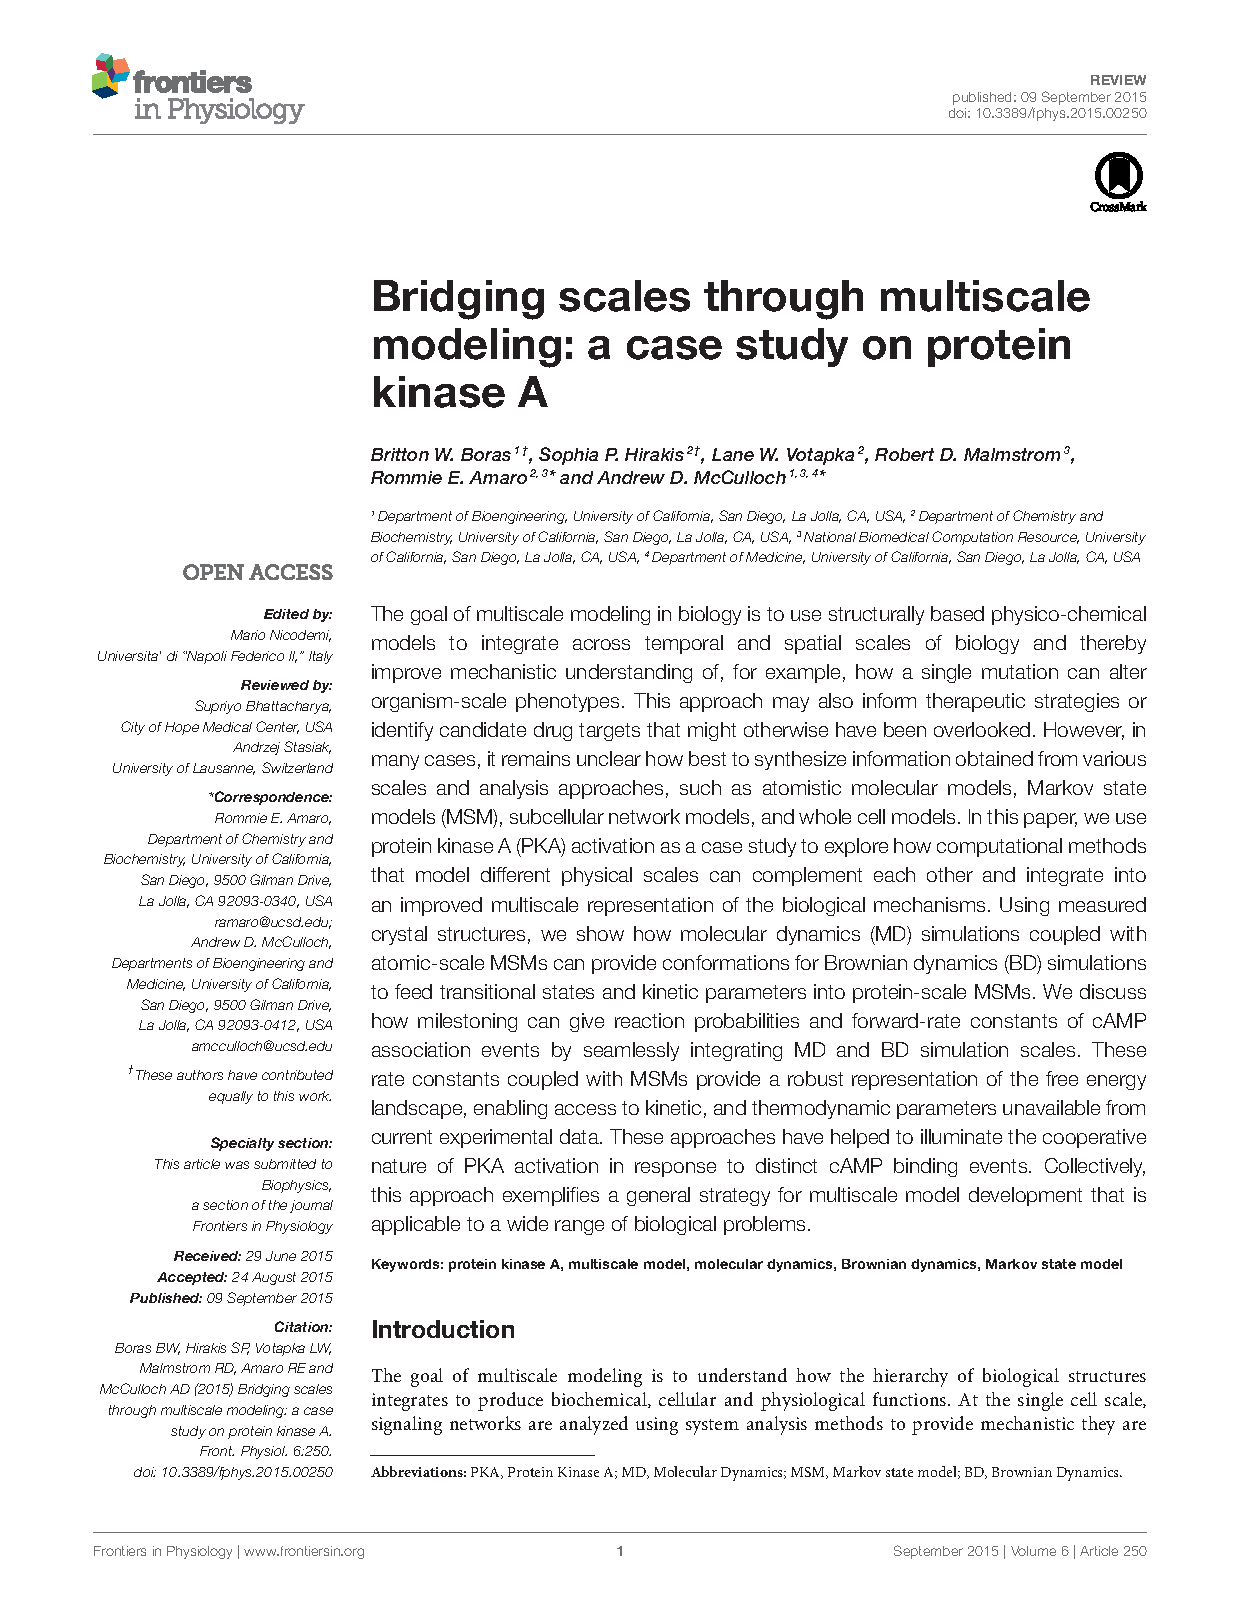
\includegraphics[height=0.82\textheight]{Frontiers_Paper_Chapter2.pdf}
In the following manuscript, we demonstrate ways in which multiscale computational methods can integrate structural and chemical information to better understand how, for example, changes in protein sequence such as point mutations can alter organ-level phenotypes like cardiac contraction. Our case study is focused on Protein Kinase A (PKA) and the manuscript provides examples of multiscale methods that compliment each other, showing how structural and kinetic information can be combined into an integrated understanding of the protein system. Included in the manuscripts are examples of how multiple short molecular dynamics (MD) simulations can be combined into an atomistic Markov State Model (MSM) to provide mechanistic insights and kinetic information about important structural transitions in the cyclic nucleotide binding domain (CBD) of PKA. Moreover, classical and accelerated  MD simulations can provide new structures to understand the association kinetics of the second messenger, cAMP using Brownian dynamics (BD) simulations.  BD simulations yield kinetic rates of bimolecular association reactions that can be used in protein-scale MSMs. Semi-analogous to MSMs are milestoning methods that have been developed and optimized in the Amaro group at the University of California San Diego that directly integrate MD and BD to understand on and off-rates of ligands to their protein systems. Finally, we discuss how the information provided by the aforementioned methods can be used in higher-order subcellular and whole cell models. 




%% Inserting the rest of the Fronteirs paper pages and add entries to LoF, LoT
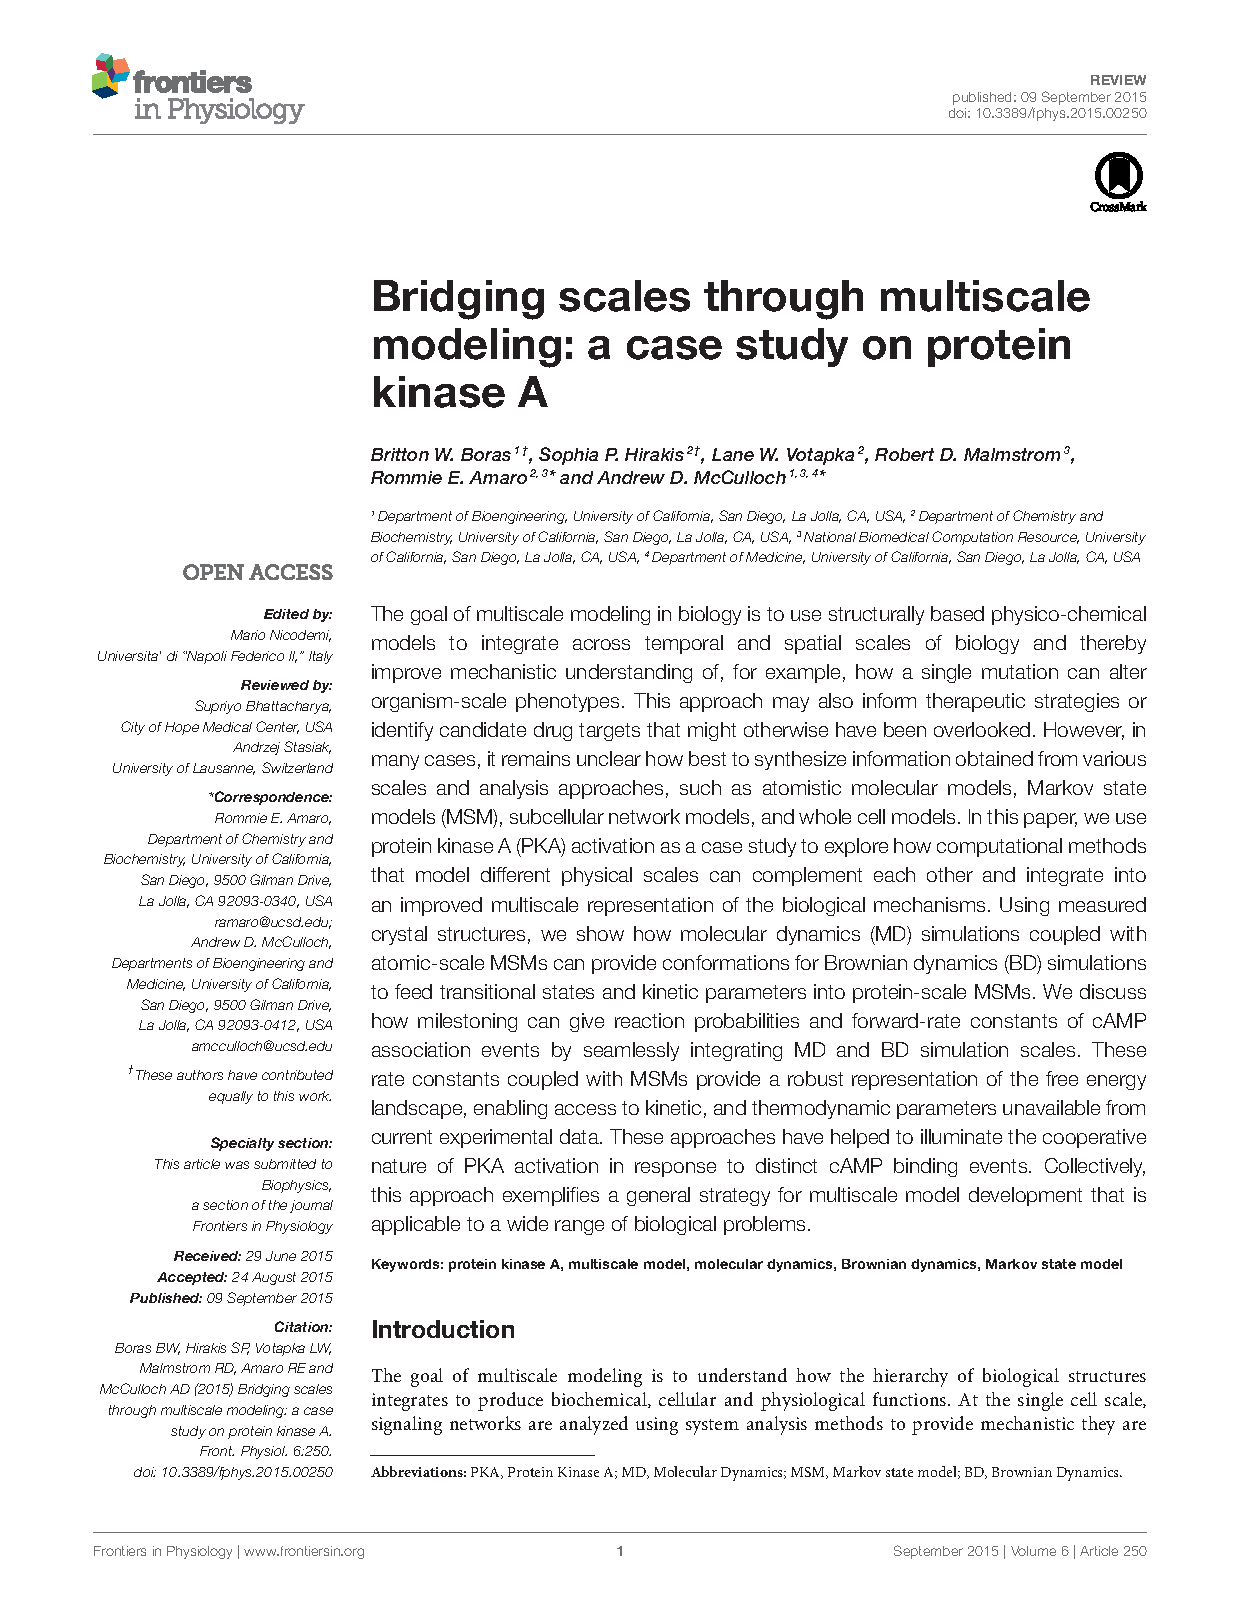
\includepdf[
  pages={-}, %% All subsequent pages
  scale=0.9,
  pagecommand={\pagestyle{myheadings}}, %% If you want to apply normal headers/footers
  %% Add to LoF and LoT. Note that the page numbers MUST be sorted.
  %  Page numbers here are _relative_ to the included PDF file itself.
  addtotoc={
    1,section,1,{Introduction},sec:intro,
    3,section,1,{Nomenclature},sec:nomen,
    3,section,1,{Accessing the Conformational Ensembles of Proteins},sec:conf,
            3,subsection,2,{Molecular Mechanics and Molecular Dynamics Simulations},sec:sub31,
            3,subsection,2,{Atomic-scale Markov State Models of a Conformational Ensemble},sec:sub32,
    5,section,1,{Investigating Intermolecular Interactions},sec:intermolec,
            5,subsection,2,{Brownian Dynamics Simulations},sec:sub41,
            5,subsection,2,{Considerations for Brownian Dynamics Simulations},sec:sub42,
            7,subsection,2,{Unifying MD and BD Simulations through Milestoning},sec:sub43,
    8,section,1,{From Atomistic to Protein-scale Models},sec:atomtoprotein,
            8,subsection,2,{Protein-scale MSM},sec:sub51,
                %8,subsubsection,3,{Functional State Discovery through MD Simulations},sec:sub52,
                %9,subsubsection,3,{Using BD Simulations to Inform Kinetics},sec:sub53,
                %9,subsubsection,3,{Testing with Empirical Data},sec:sub54,
            9,subsection,2,{Applying MD and BD modeling to Protein Scale PKA-RI$\alpha$ MSM},sec:pkamsm
            },
  addtolist={
    2,figure, {Bridging gaps through multiscale modeling},fig:bridginggaps,
    3,scheme, {Activation Mechanism of PKA RI$\alpha$ with Different R conformations and Relative Association Rates}, fig:wide,
    4,figure, {Protein Kinase A cyclic nucleotide binding domain Markov state model}, figure:pkacbdmsm,
    6,figure, {Brownian dynamics simulation method}, figure:bd,
    8,figure, {Milestoning applied to unite MD and BD}, figure:MDBDmilestoning,
    10,figure, {The Markov State Model of PKA-RI$\alpha$ R$_{2}$C$_{2}$ holoenzyme}, figure:milestoning
  }%,
%  addtotoc={
%    2, section=1, subsection=0, {Test}, label:testtest
%    }
  ]{Frontiers_Paper_Chapter2.pdf} %%PDF to insert

\section{Acknowledgments}
Chapter 1, in full, is a reprint of the material as it appears in Frontiers in Physiology 2015. 
Boras, Britton W.; \textbf{\underline{Hirakis, Sophia P.}}; Votapka, Lane W.; Malmstrom, Robert D.; Amaro, Rommie E.; McCulloch, Andrew D.;"Bridging scales through multiscale modeling: a case study on protein kinase A," Frontiers in Physiology, 6: 250, 2015. 
 The dissertation author was the co-primary author of this paper.

This work was the result of a direct collaboration with wonderful co-authors whom I would like to formally acknowledge. Dr. Britton W. Boras, is the co-first author who wrote a portion of the paper and created figures used in the manuscript. Dr. Lane W. Votapka and Dr. Robert D. Malmstrom also wrote sections of the paper and helped to construct figures. Dr. Rommie E. Amaro and Dr. Andrew D. McCulloch provided support for the manuscript through editing and revision of the text. I extend my gratitude to the above-mentioned scientists for their creative and scientific contributions to the manuscript. 


%End of Chapter 1

%~~~~~~~~~~~~~~~~~~~~~~~~~~~~~~~~~~~~~~~~~~~~~~~~~~~~~~~~~~~~~~~~~~~~~~~
%Beginning of Chapter 2
\chapter{Visualizing and understanding protein-protein interactions with Molecular Dynamics}\label{cosmo_paper}
\vspace*{-1cm}
The following manuscript demonstrates the ways that protein-protein contacts involved in bacterial infectious mechanisms can be elucidated by protein crystallography and further understood using MD simulations. The subject of the manuscript, Group A \textit{Streptococcus} (GAS), is incredibly infectious with a wide range of symptoms ranging from sore throat to flesh-eating bacteria that affects the skin and internal organs such as the heart. Development of a vaccine treatment for GAS has been slow due to the large variance in sequence of its surface antigen, the M protein. Over 200 different types of M proteins have been identified and antibodies recognize a hypervariable region (HVR) of the M protein, offering narrow specificity due to sequence variability. The infectious mechanism of the protein is quite remarkable, as the Human C4b-binding protein (C4BP) interacts with around 90\% of M proteins, making it a great candidate for understanding the broad specificity of the HVR. In this study, crystal structures of C4BP in complex with four different M-proteins reveal the uniform and sequence-variant "tolerant" reading head of the protein-protein complex. 

In context of the thesis, this manuscript demonstrates how observations made by crystallographic methods are enhanced by molecular simulation. The MD study in this manuscript allowed us to visualize and understanding of the atomistic contacts which could not be explained by the static structure itself.
A number of mutants of the WT, which strengthened and weakened the contacts of the M protein-C4BP complex.  Most notably, the MD showed how water is able to penetrate the protein complex due to a point mutation of a hydrophobic reside and how charged reside mutations counter-intuitively strengthen the interactions between C4BP and M protein complexes.   \\

\newpage
\includegraphics[height=0.79\textheight]{Buffalo_MainText.pdf}
\includepdf[
	pages={2-},
	scale=0.9,
	pagecommand={\pagestyle{myheadings}},
	addtolist={
    15,figure, {Structures of M-C4BP complexes},fig:C4BPstructures,
    16,figure, {C4BP Binding Mode},fig:bindingmode,
    17,figure, {C4BP-binding modes of M proteins},fig:mproteinbindingmode,
    18,figure, {M2-C4BP interaction},fig:interaction,
    19,figure, {Schematic of M protein domains},fig:domains,
    20,figure, {Electron density for the M49 HVR-C4BP$\alpha$1-2 complex},fig:electrondensity,
    21,figure, {Structure of M22-C4BP},fig:m22structure,
    22,figure, {Structure of M28-C4BP},fig:m28structure,
    23,figure, {Structure of M49-C4BP},fig:m49structure,
    24,figure, {Coiled coil parameters of M proteins},fig:coilcoil,
    25,figure, {Rotation of C4BP$\alpha$1-2},fig:rotation,
    26,figure, {Structure of the M22-C4BP interaction in which C4BP$\alpha$1 is tilted rather than rotated},fig:tilt,
    27,figure, {Sequence alignment of C4BP-binding M protein HVRs of the M2/M49 pattern},fig:alignmentM2M49,
    28,figure, {Sequence alignment of C4BP-binding M protein HVRs of the M22/M28 pattern},fig:alignmentM22M28,
    29,figure, {C4BP-binding M protein HVRs that cannot be classified as belonging to either M2/M49 or M22/M28 patterns},fig:hvr,
    30,figure, {C4BP-M2 interaction},fig:interactions,
    31,figure, {Molecular dynamics simulation of the Arg39 ‘hydrophobic nook’ interaction with wild-type M2 and M2 F75A},fig:MD,
    32,figure, {Interactions of M2 and M2 (K65A/N66A) with C4BP$\alpha$2},fig:interactions2,
    33,figure, {B-factors of C4BP$\alpha$2 bound to M2 or M2 (K65A/ N66A)},fig:bfactor,
    34,figure, {Uncropped Gels},fig:gels,
    35,table, {Data collection, phasing and refinement statistics for native and SAD (SeMet) structures},table:crystal,
    36,table, {Ionic Interaction Pair Occupancy in C4BP$\alpha$2 for Quadrilateral Residues of M2},table:occupancy1,
    36,table, {Ionic Interaction Pair Occupancy in Quadrilateral for Residues of M49, M22, and M28},table:occupancy2
  	}
 ]{Buffalo_MainText.pdf}


\section{Acknowledgment}
Chapter 2, in full, is pre-publication print of an article published in Nature Microbiology 2016. 
Buffalo, Cosmo Z.; Bahn-Suh, Adrian J.; \textbf{\underline{Hirakis, Sophia P.}}; Biswas, Tapan; Amaro, Rommie E.; Nizet, Victor; Ghosh, Partho; "Conserved Patterns hidden within group A Streptococcus M protein hypervariability are responsible for recognition of human C4b-binding protein." The dissertation author was the third author of this paper.

This work was the result of a direct and indirect collaboration with a collection of scientists whom I would like to acknowledge. My dear friend and colleague, Dr. Cosmo Z. Buffalo and I began our computational investigations of the M-proteins in complex with Human C4BP, albeit without the blessing of our advisors. He is responsible for the crystallographic characterization of the four complexes as well and wrote the manuscript. Adrian J. Bahn-Suh is Cosmo's student who also assisted with the experimental components of the work and figures. Dr. Tapan Biswas, a scientist on the project, assisted Cosmo in the refinement of the structures. My beloved advisor, Dr. Rommie E. Amaro, advised me on the data analysis and helped to write and revise the manuscript. Though not an author on the paper, Pek Ieong, a former scientist in the Amaro lab, provided invaluable advice for the analysis of the binding regions through fingerprinting algorithms that she developed using Kepler software. Dr. Victor Nizet and Dr. Patho Ghosh helped write the manuscript and advised on scientific studies to further refine the work. I thank them all humbly for welcoming my computational insights and for allowing me to collaborate on this wonderful project. 

%~~~~~~~~~~~~~~~~~~~~~~~~~~~~~~~~~~~~~~~~~~~~~~~~~~~~~~~~~~~
%Beginning of Chapter 3
\chapter{Bridging structural and mechanistic observations with computational modeling techniques}\label{first:paper}
\vspace*{-1.2cm}
In the following manuscript, we demonstrate how two distinct scales of molecular simulations can be used to understand the structure of a protein complex and suggest paths for the activation mechanism by a small molecule regulator. The subject of the manuscript is the RI$\alpha$ heterotetrameric complex of Protein Kinase A (PKA). PKA is a ubiquitous eukaryotic protein responsible for turning proteins on and off in response to an extracellular stimulus. PKA is comprised of two catalytic (C) subunits that phosphorylate protein targets and regulatory (R) subunits (R$_{2}$C$_{2}$). Each R subunit has two Cyclic-nucleotide binding Domains (CBD), which bind a total of four equivalents of cAMP for each R dimer. Upon binding cAMP, the inhibition of the catalytic subunits is relieved through dissociation, and the C subunits are free to phosphorylate protein targets. The holoenzyme structure has been the subject of some controversy. Specifically, the interface between the Type 1A R and C subunit has been debated extensively by those in the PKA community. Solution-structure methodologies such as small-angle X-ray scattering (SAXS) and Hydrogen/Deuterium exchange Mass Spectrometry (H/DxMS) suggest a protein-protein interface that involves mostly CBD-A. Crystallography of the full-length R in the holoenzyme complex proved challenging for the wild-type PKA, but a CBD-B mutant of R described a more-extensive interface that involved both CBD-A and CBD-B.

In this manuscript, MD simulations helped bridge the gap between information obtained from crystallographic and solution structures, revealing a stable conformation of the R subunit that was elucidated after only a few nanoseconds of simulations starting from the extended conformation of the R subunit in the crystal structure. In the wild-type form, the R subunit relaxes into a conformation which we named the Flipback conformation. With the new R subunit structure, a model of the heterotetramer was constructed and proved extremely consistent with the solution structure description. More specifically, the Flipback structure is consistent with solvent-exposure of the C subunit determined by H/DxMS and the shape of the molecule determined by SAXS. 

Using the flipback model of the heterotetramer, we used Brownian Dynamics (BD) to investigate the differential association kinetics of the small-molecule regulator cAMP to the two proposed structures: 1) the (Holo) holoenzyme model derived from two crystal structures and 2) the Flipback model derived from our simulations and based on a crystal structure model of the heterotetramer. Earlier studies determined that cAMP preferentially binds to CBD-B. This observation was confirmed by our BD simulations. A novel insight from the simulations was the association to the A-domain. In the heterotetrameric Flipback conformation, the association of cAMP to CBD-A was two orders of magnitude higher than to CBD-A of the crystallographic "Holo" model. In the heterodimeric forms, the association difference was more pronounced, with four orders of magnitude higher association rates to the Flipback conformation over the Holo conformation. The difference in association kinetics is due to a re-distribution of the electrostatic charges as a result of the conformational differences between Holo and Flipback states. The electrostatic potential on the surface of the protein is responsible for the long-range attractive forces guide cAMP to the CBD target. These findings suggest that the R subunit may adopt the Flipback conformation in order to bind cAMP in the A domain of PKA. With these new insights from computational simulations, we have a better understanding of the heterotetrameric structure of PKA, bridging the gap between solution and crystallographic observations.    \\
%% Inserting the first page of the  Flipback paper as an image
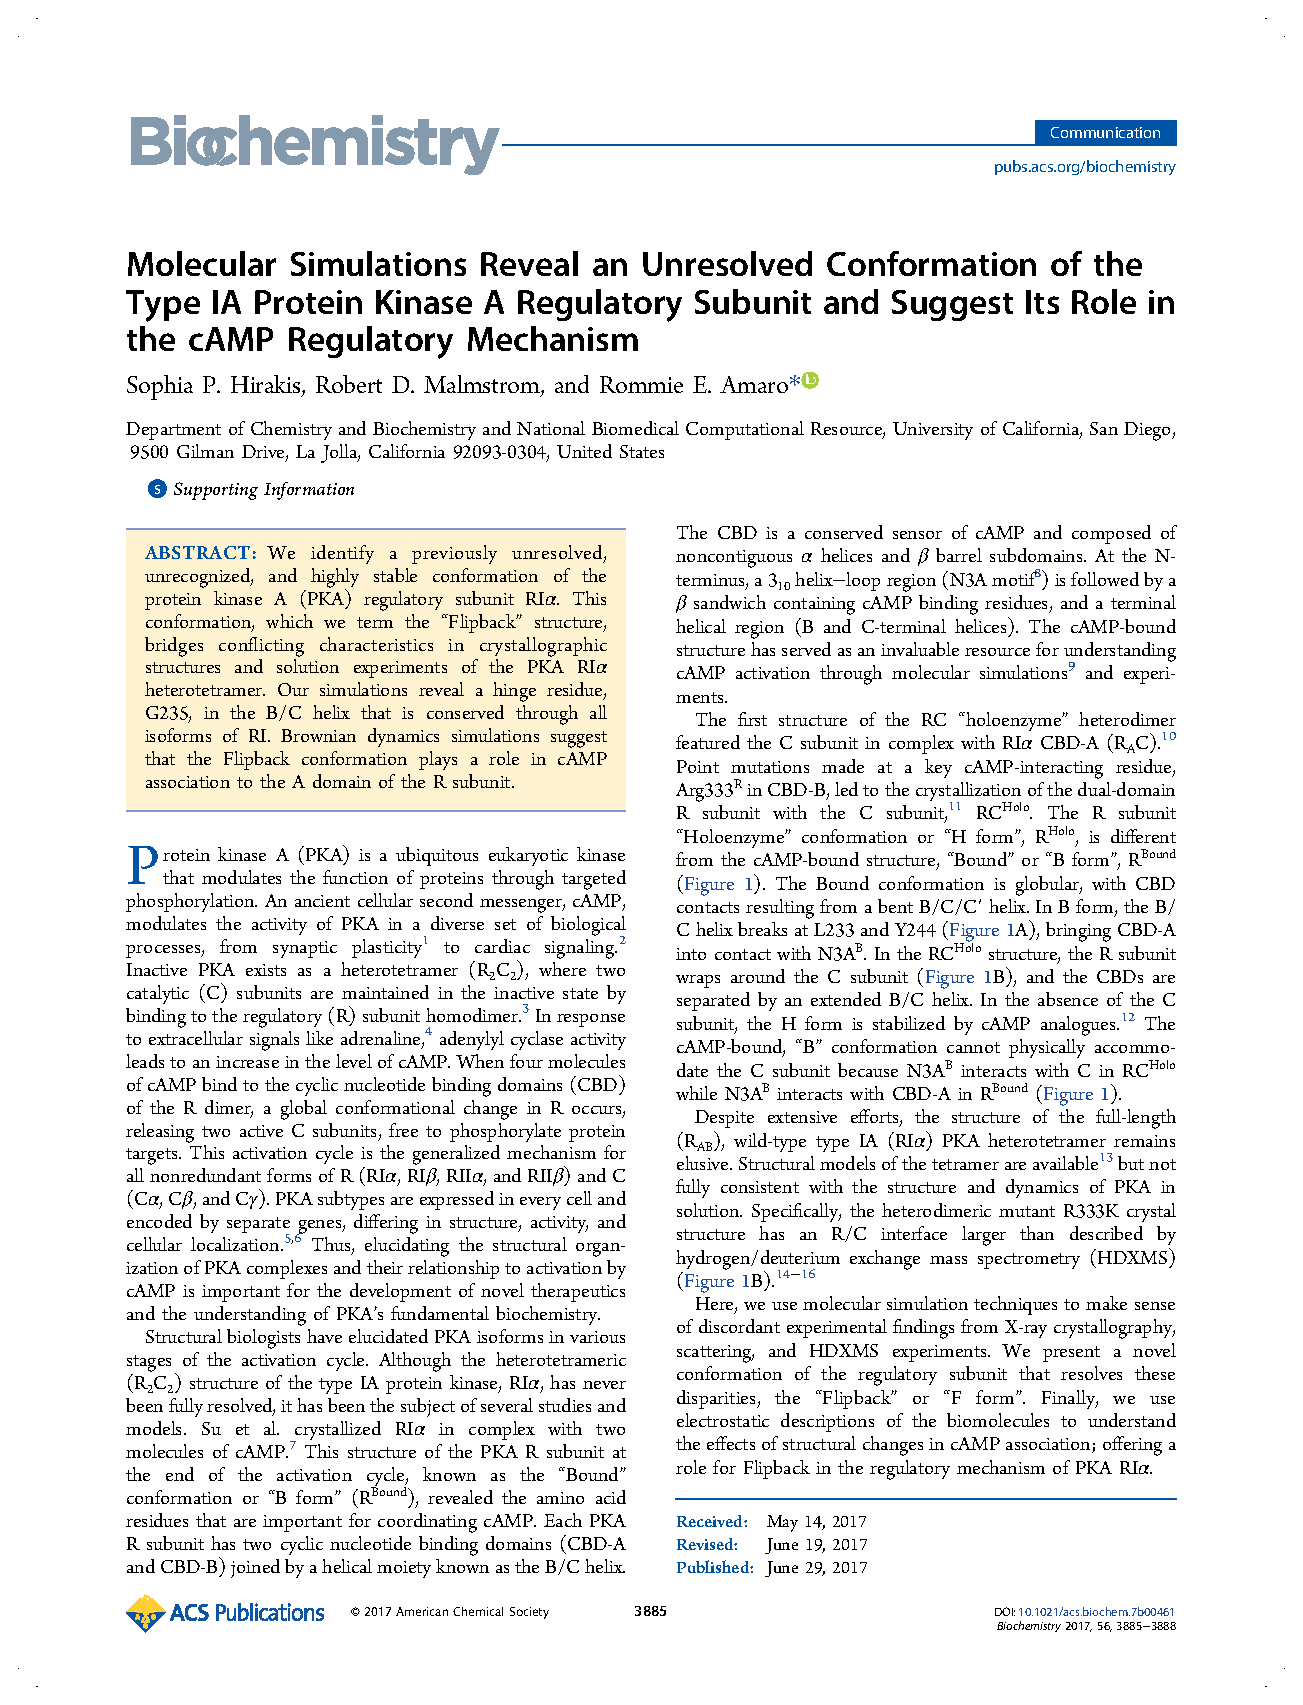
\includegraphics[height=1\textheight]{Flipback_Paper_Chapter3.pdf}

%% Inserting the rest of the Flipback paper pages and add entries to LoF, LoT
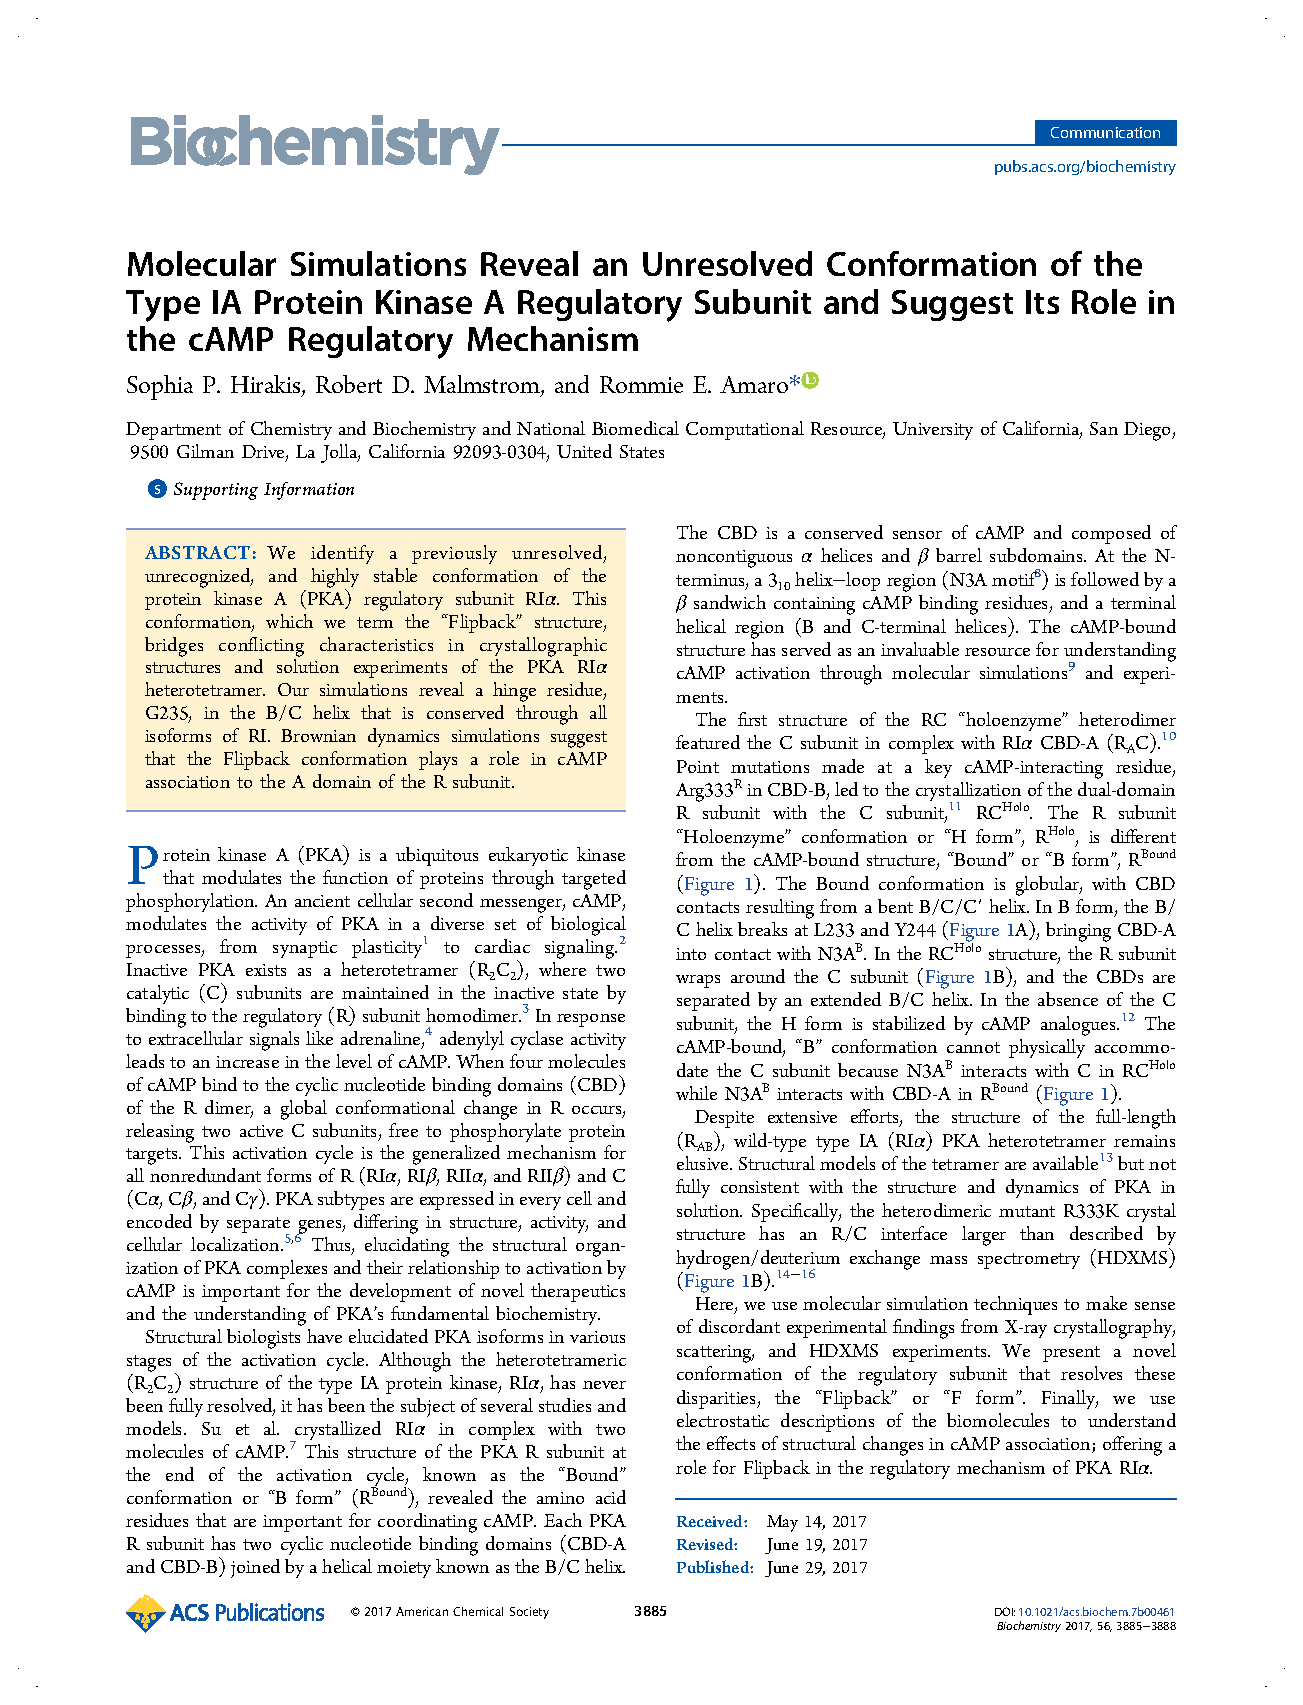
\includepdf[
  pages={2-}, %% All subsequent pages
  scale=0.9,
  pagecommand={\pagestyle{myheadings}}, %% If you want to apply normal headers/footers
  %% Add to LoF and LoT. Note that the page numbers MUST be sorted.
  %% Page numbers here are _relative_ to the included PDF file itself.
  addtolist={
    3,figure, {Comparison of the novel Flipback heterodimer with resolved PKA RI$\alpha$  Conformations},fig:comparison,
    2,table, {Rates of Association if cAMP with Cyclic Nucleotide Binding Domains of PKA complexes}, table:rates
  }
 ]{Flipback_Paper_Chapter3.pdf} %%PDF to insert



%% Inserting the first page of the  Flipback supplemental paper as an image
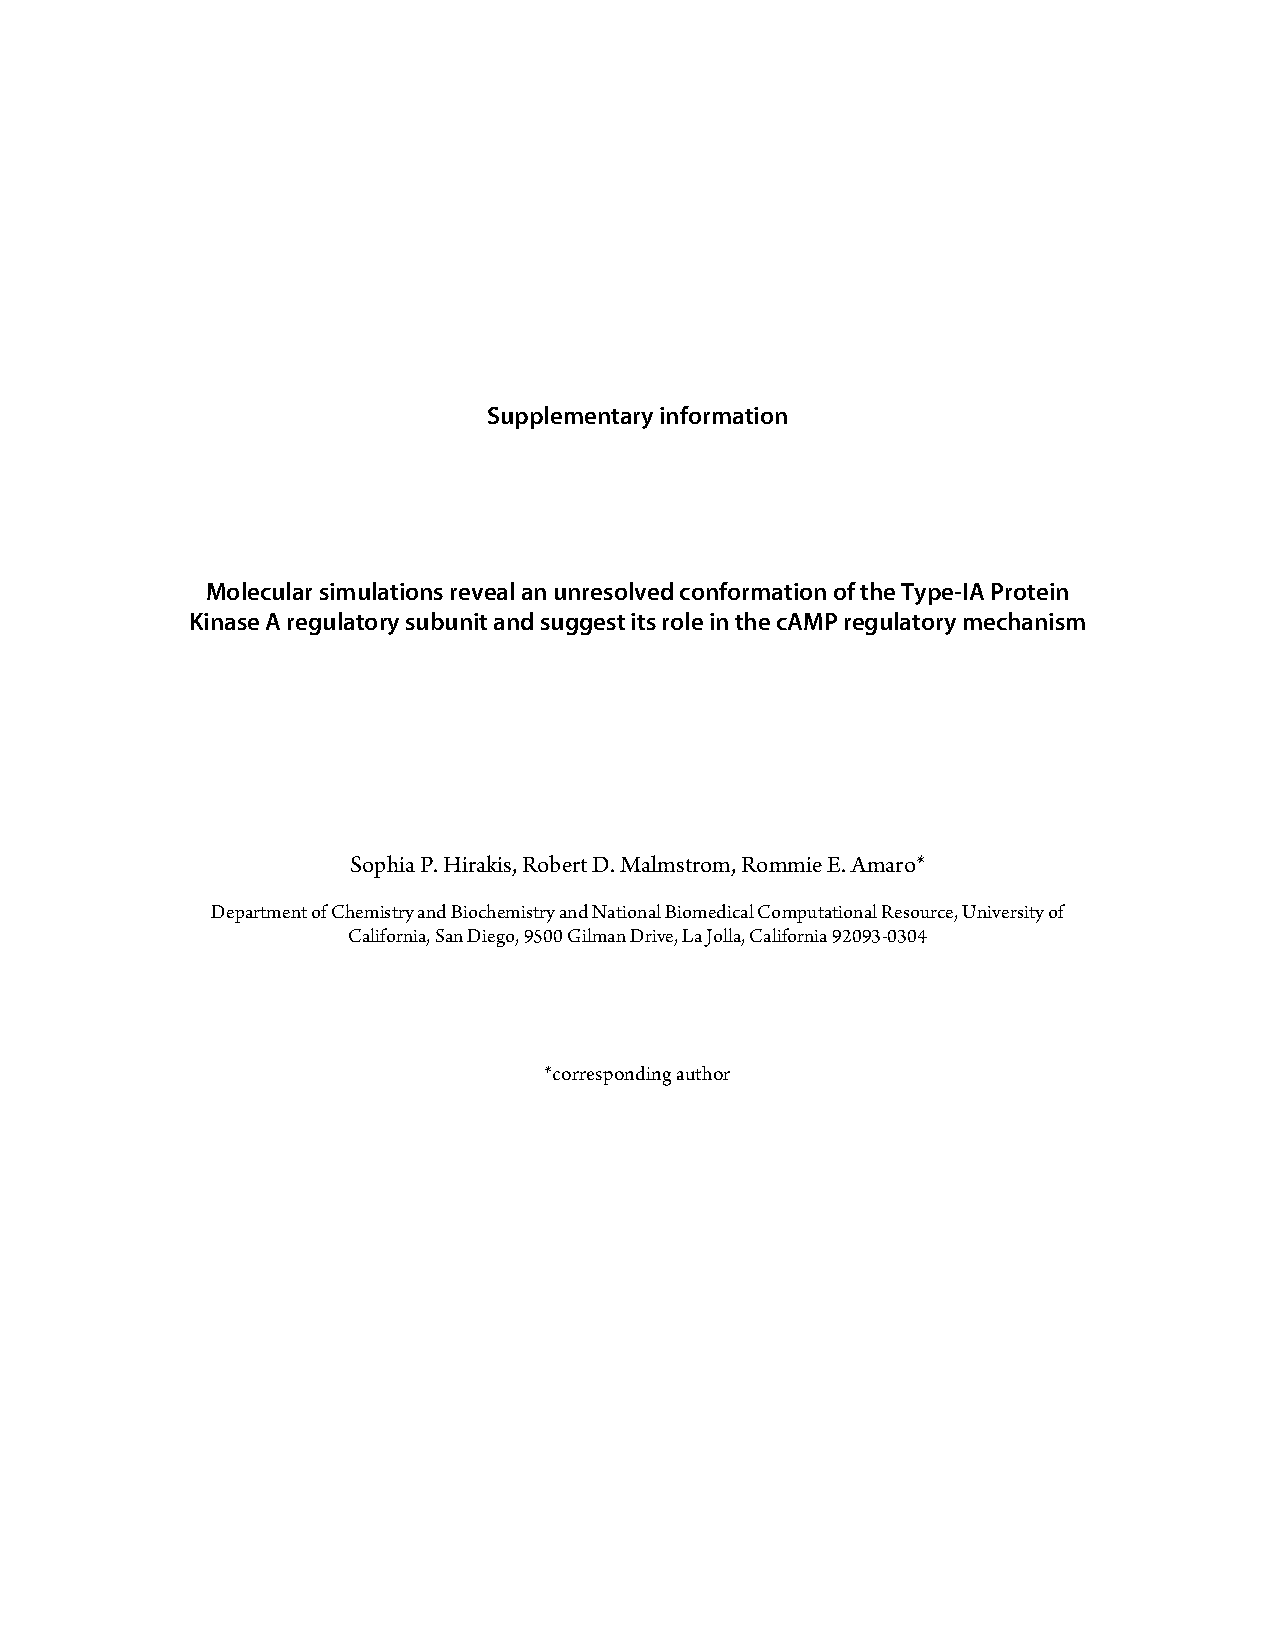
\includegraphics[height=0.8\textheight]{Flipback_Supplemental_Chapter3.pdf}

%% Inserting the rest of the Flipback paper pages and add entries to LoF, LoT
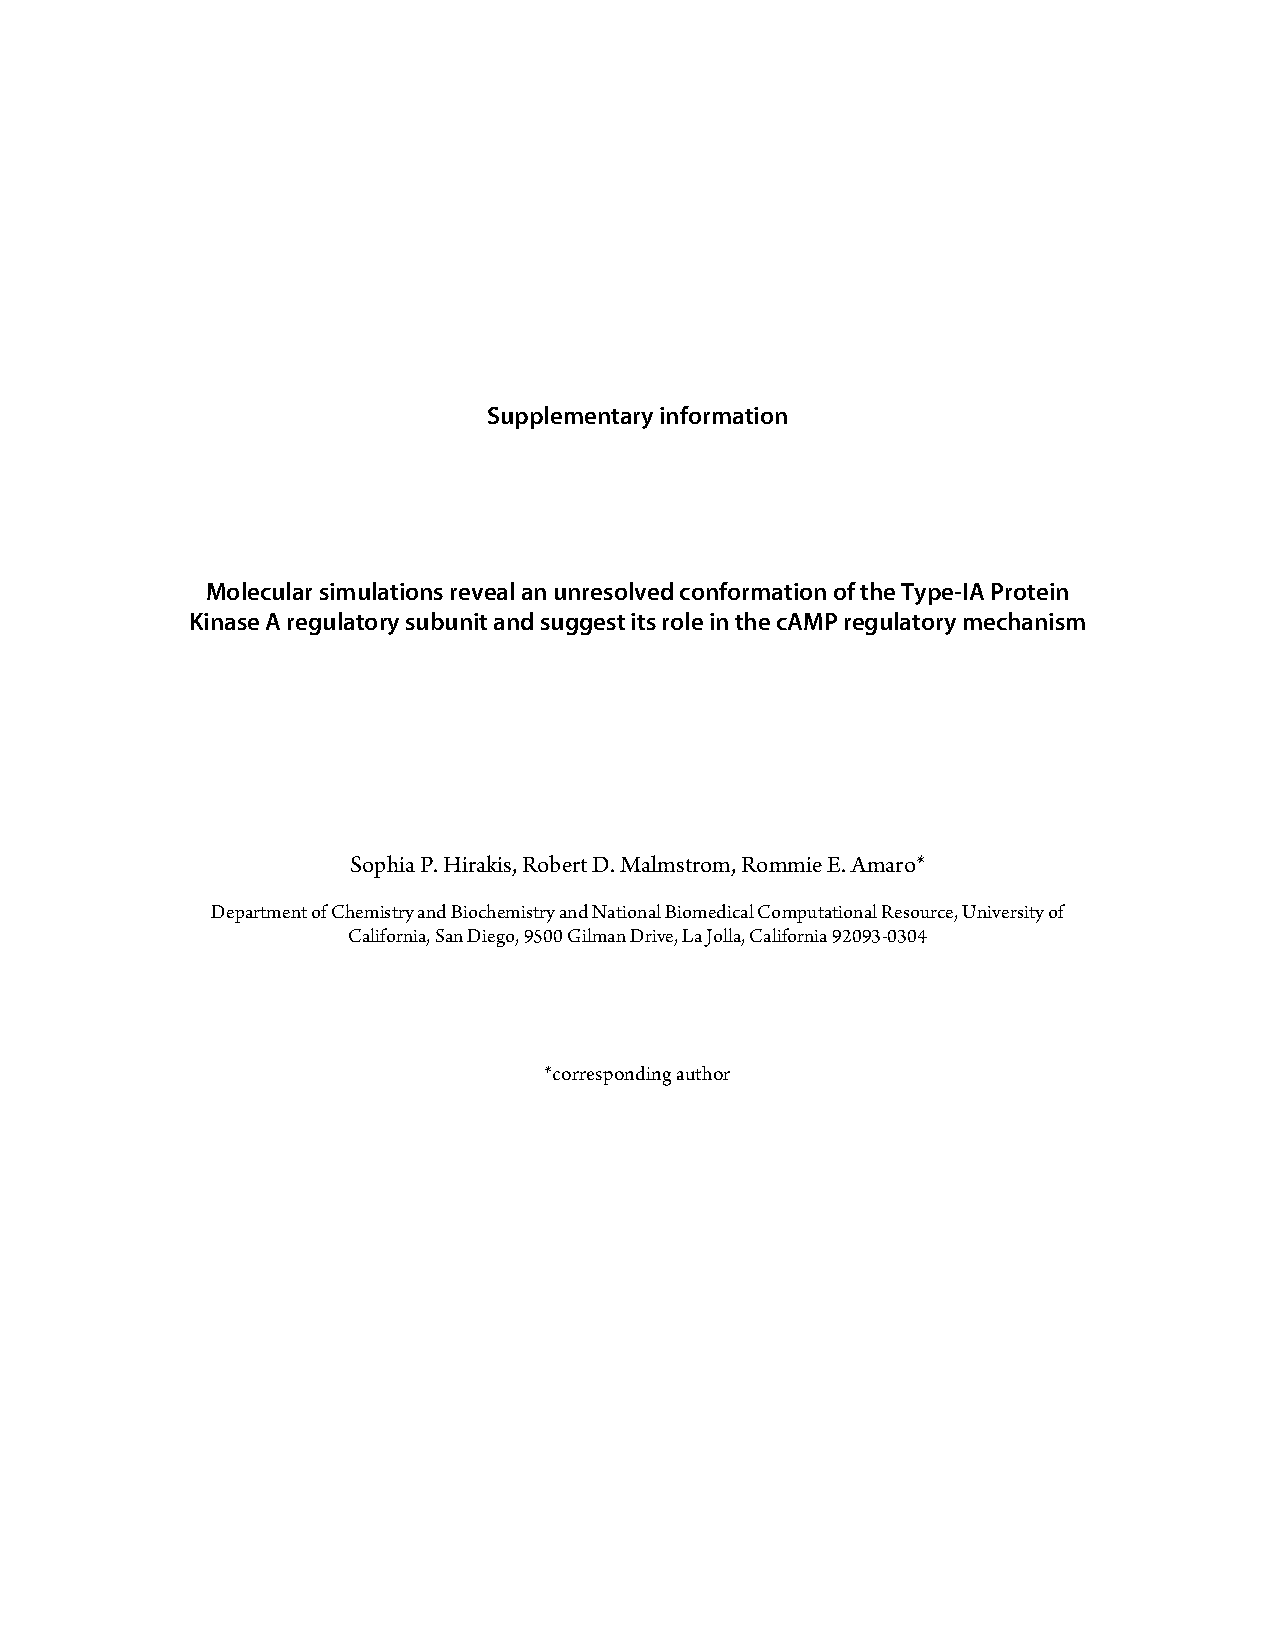
\includepdf[
  pages={2-}, %% All subsequent pages
  scale=0.9,
  pagecommand={\pagestyle{myheadings}}, %% If you want to apply normal headers/footers
  %% Add to LoF and LoT. Note that the page numbers MUST be sorted.
  %% Page numbers here are _relative_ to the included PDF file itself.
  addtolist={
    3,figure, {The stability of the Flipback conformation},fig:stableflipback,
    4,figure, {Generalized encounter compled of cAMP and the CBD-A/B},fig:encountercomplex,
    4,table, {Encounter Complex Description of R subunit and cAMP},table:rates,
    4,figure, {Atomic numbering and naming of cAMP molecule in BD simulations},fig:cAMPnumbers,
    5,figure, {Electrostatic descriptions of the four systems},table:rates
  }
]{Flipback_Supplemental_Chapter3.pdf} %%PDF to insert



\section{Acknowledgment}
Chapter 3, in full, is a reprint of the material as it appears Biochemistry 2017. 
\textbf{\underline{Hirakis,}}\ \textbf{\underline{Sophia P.}}; Malmstrom, Robert D.; Amaro, Rommie E.; "Molecular Simulations Reveal an Unresolved Conformation of the Type IA Protein Kinase A Regulatory Subunit and Suggest its Role in the cAMP Regulatory Mechanism." The dissertation author was the primary investigator and author of this paper.

This discovery would not have been possible without the original simulations by Dr. Robert D. Malmstrom. Dr. Malmstrom allowed me to analyze his simulations and through this, I discovered the Flipback conformation. Dr. Malmstrom assisted in the manuscript review. Though not listed as an author, special thanks goes out to Dr. Alexandr Kornev who assisted in the understanding of the Flipback conformation in the context of the existing literature on PKA heterotetramer. He provided critical edits to the document which helped project it towards success and acceptance in the field. Dr. Susan S. Taylor provided insights and I thank her for the many conversations about this. Dr. Lane W. Votapka and Dr. Gary Huber assisted with the construction of the BrownDye simulations and for this, I thank them. Dr. Jamie M. Schiffer helped understand the SAXS profiles of PKA tetramer. Dr. Elizabeth Komives provided support for the discovery of the structure and much welcomed enthusiasm for the publication of the manuscript. Finally, I thank my beloved advisor, Dr. Rommie E. Amaro for pushing me to publish this work and for helping me to see the value in my findings, which the world may never have known of if not for her invaluable encouragement. Thus, cardiac function spans multiple scales of space and time, from that which can be seen with the naked eye, to that which only a computational microscope can observe.

%End of Chapter 3

%~~~~~~~~~~~~~~~~~~~~~~~~~~~~~~~~~~~~~~~~~~~~~~~~~~~~~~~~~~~~~~~~~~~~~~~

%Beginning of Chapter 4


%...
\chapter{Subcellular spatial modeling in realistic geometries with stochastic particle methods to understand heart disease}
\section{Abstract}
The evasive source and cause of diseases is oftentimes \textit{smaller than you think}. Imagine, though, chasing something that you can't actually \textit{see}. This is the plight of almost all scientists whose study does not involve the use of a microscope. Fortunately for the modern-day biomedical scientist, computational advancements harnessing the near-limitless potential of mathematics in the language of physics are able to \textit{see the unseen}.
Computational microscopy is a tool developed by thousands of talented scientists that yields the power of visualization to the scientist seeking to visually understand biological systems. With progressive advancements in the power of computer graphics and the development of mathematical theories to explain biological behavior, computational microscopy is a term given to a collection of methods developed by hundreds of scientists throughout the greater half of the last century. Using this powerful tool, the artist within the scientist is able to visualize what they know in their mind's eye to be true through their experiments. It also allows scientific discoveries to be translated without the explicit use of language. With respect to diseases, the culprit is oftentimes an atomic-level alteration that has a butterfly effect throughout the cell, scaling up through space and time to affect organs and eventually, the whole organism. In accordance with its name, the computational microscope not only allows us to visualize extremely small entities like atoms, molecules, proteins, cells, and the like. But it is especially unique, as it allows us to move through time in order to understand the dynamics of the system we seek to "see". Like a biophysically detailed time-lapse, we are able to \textit{see through time}, the development of a microscopic system and compare how small changes can have large-scale effects. 


\section{Introduction}
 Over 135 years ago, Dr. Singer demonstrated that a human heart would not beat in the absence of Ca\textsuperscript{2+} ions \cite{Ringer1883}. Yet, human heart is the size of a fist. Thus the process of the heartbeat is an inherently multiscale process. The atria and ventricles of the heart make up the "working chambers" which pump oxygenated blood through the body, and deliver deoxygenated blood to the lungs. The thickness of these walls are several millimeters depending on the region of the heart. Each cell is a complicated but regular structure of membranous invaginations that range from 20-450 nm in diameter. Cardiomyocytes, or muscle cells, contain bundles of muscle fibers that are responsible for the contraction of the heart. The thick filaments are made out of myosin protein and are about that are 160-170 \si{\angstrom} in diameter while thinner actin filaments are 6 to 10\si{\angstrom} in diameter. Finally, large proteins in close contact with each other (roughly 20 nm) sense calcium ions (roughly 231 pm radius), triggering processes the contraction and relaxation of muscle fibers, resulting in the beating of the heart. Thus, cardiac function spans scales that can be observed with the naked eye, to invisible phenomena that only a computational microscope can see.  

 A healthy heart contracts in response to a synchronous electrical stimulation of the plasma membrane, also known as the sarcolemma, initiated by the sinoatrial (SA) node. The membrane action potential travels from the SA node and is propagated from cell to cell through gap junctions\cite{Bernstein2006}. This electrical stimulation results in membrane depolarization, to which the cell responds with a muscular contraction, a phenomenon known as  excitation-contraction coupling (ECC)\cite{Cheng1994}. 
 
 Cardiomyocytes have specialized structures within which this process occurs. Invaginations in the sarcolemma (cell membrane), known as axial and transverse-tubules (TT) are positioned directly adjacent to the sarcoplasmic reticulum (SR), the intracellular calcium store. Depolarization of the sarcolemma activates and opens L-Type Calcium Channels (LTCC), through which calcium enters the cell. The LTCC are in close proximity large ($>2$MDa) SR membrane proteins called Ryanodine Receptors (RyR) \cite{Lanner2010}. The space between the extracellular membrane and SR membrane is known as the dyadic junction and \textit{this is where the magic happens}.

High calcium concentrations in the extracellular matrix cause influx of Ca\textsuperscript{2+} through LTCC, into the cardiac muscle cells which maintain a very low Ca\textsuperscript{2+}  concentration. Directly adjacent to LTCC are RyR, which are regulated by more than 30 proteins\cite{Fill2002}. When RyR sense changes in cytosolic calcium, a \textit{signal amplification} results, whereby RyR release thousands of Ca\textsuperscript{2+} ions from the SR into the cell, an event known as a triggered calcium spark or Calcium Induced Calcium Release (CICR). In response to the change in cytosolic Ca\textsuperscript{2+}, the inhibition of action and myosin is relieved by Troponin C (TnC) which directly bind Ca\textsuperscript{2+}. This causes the muscle fiber proteins to slide across each other leading to muscle fiber shortening, or muscular contraction that squeezes blood out of the atrial chambers of the heart into the ventricles and out towards the rest of the body. An important SR protein, the Sarco/Endoplasmic Reticulum Ca\textsuperscript{2+}-ATPase (SERCA) pump, clears the cytosol of the high Ca\textsuperscript{2+} levels, allowing for muscle relaxation. This cycle is repeated every time the heart beats.

Early on, LTCC (also known as Dihydropyridine Receptors, and Voltage-Dependent Calcium Channels) \cite{Lu1994} and RyR \cite{Stern1999} were implicated in the generation of calcium sparks. Though theories about ECC existed \cite{Stern1992}, the first Ca\textsuperscript{2+} spark event was visualized and confirmed 25 years ago using laser-scanning confocal microscopy \cite{Cheng1993} and quickly confirmed in subsequent studies \cite{Cannell1994,Cannell1995}. Within a few years, computer simulations were applied to this system to model the elementary events responsible to elucidate the subcellular mechanisms responsible for what was visualized with the early fluorescence measurements \cite{Cannell1997}.

Microscopic fluorescence imaging techniques have limitations in terms of their ability to resolve spatial changes in calcium levels; especially at short space and timescales. Therefore, computational models have played an important role to tease out important features of CICR and ECC. The field of computational cardiology has an impressive track-record of over 30 years of computational modeling of cardiac excitation phenomena that have explained and predicted mechanisms that underlie calcium signaling\cite{Maleckar2017}. Almost all of the existing models use idealized geometries of myocardium that do not encapsulate the structural complexities of cardiac cells. Moreover, the field largely uses continuum approaches to model the dynamics of cardiac systems. At low molecular concentrations such as those exhibited in the cardiomyocyte.

The first use of stochastic, explicit-particle simulations with MCell to investigate cardiac Ca\textsuperscript{2+} signaling mechanisms was performed by Koh et al. in 2006\cite{Koh2006}. Their study showed the effects of altering dyadic distances had a pronounced effect on Ca\textsuperscript{2+} SR fluxes. It featured the use of simplistic planar geometries to model the SR and plasma membrane, but paved the way for future discrete-modeling methods in cardiac systems. In 2012, Hake et al. debuted the first subcellular model of a Ca\textsuperscript{2+} spark \cite{Hake2012} using realistic geometries of a cardiac calcium release unit \cite{Hayashi2009}. The methods used in the study were continuum-based and deterministic, and modeled phenomenological calcium activation. 

In the present study, we combine the realistic geometries used by Hake et al. with stochastic models approaches using particle-based, spatial reaction-diffusion modeling methods\cite{Koh2006} by Koh to debut the first-ever model of discrete calcium dynamics in realistic geometries of mouse myocardium. We use our model to investigate the effects of disease phenotypes, such as T-Tubule deformation\cite{Louch2010}, RyR dispersion\cite{Kolstad2018}, and alterations of the mouse action potential\cite{Morotti2014} on calcium signaling. 


 \section{Methods}
 
 \subsection{Building the Geometric Model}
 
 The our model builds upon and extends the model built by Hake et al. \cite{Hake2012}, which was the first to use electron tomography-derived geometries for calcium spark simulations. We used the same realistic geometry of the calcium release unit (CRU) imaged by Hayashi et al. \cite{Hayashi2009} which were segmented by IMOD \cite{Mastronarde2008} and meshed with GAMer \cite{Yu2008,Lee2018}. The geometry files were graciously provided to us through correspondence with Dr. Johan E. Hake, the primary author of the original realistic CRU paper \cite{Hake2012}. We were also very fortunate to have access to the original EM images through the local National Computational Microscopy Imaging Resource (NCMIR) at UCSD. Although the original segmented images did not include the explicit locations of the Ryanodine Receptors (RyR) in the junctional SR, images of the locations were graciously provided to us by Masahiko Hoshijima of NCMIR. In total, 96 RyR were observed in the original CRU tomograms and this number of RyR were used in our simulations and manually placed in the CRU.
 
The geometry features a contiguous sarcoplasmic reticulum (SR), two mitochondria, and one axial and one transverse tubule (TT1 and TT2 respectively). In order for the geometry mush to be usable by our simulation interface and simulation engine, (CellBlender and MCell) it was necessary to further refine the mesh. For this, we used an improved version of GAMer developed locally at the National Biomedical Computational Resource (NBCR) at UC San Diego (UCSD) \cite{Yu2008,Lee2018}.

\begin{figure}
\centering
	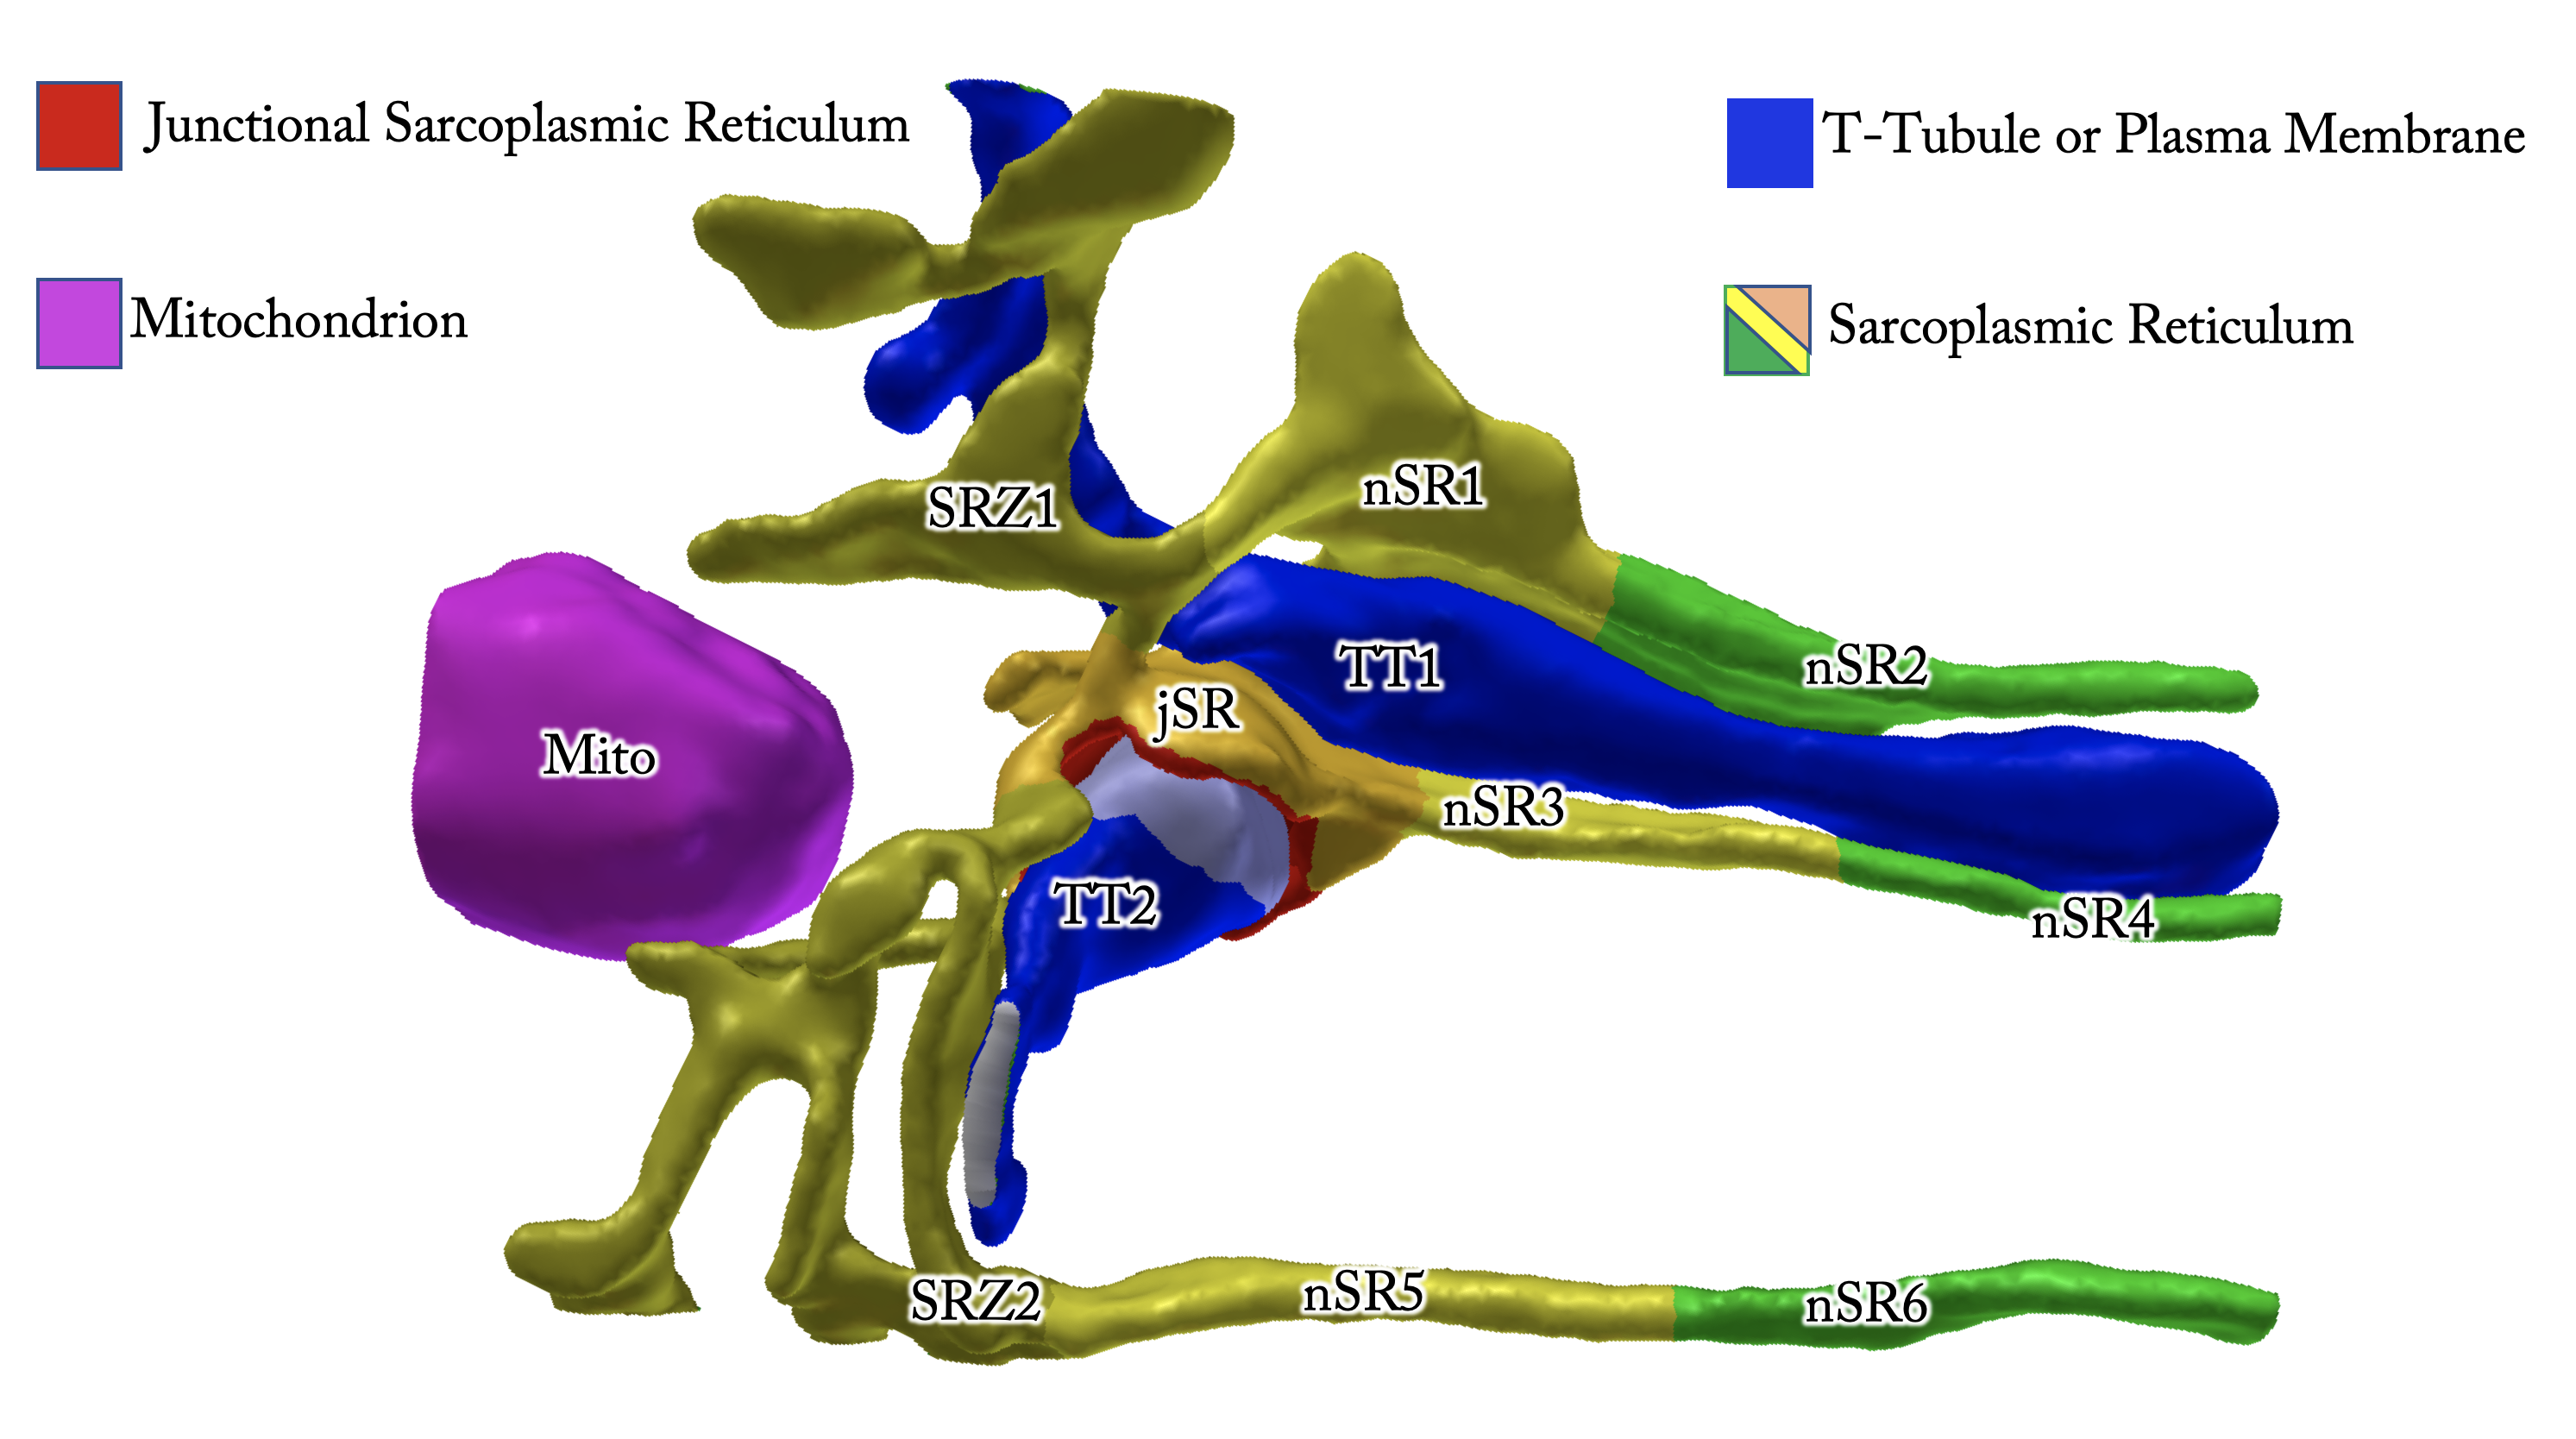
\includegraphics[scale=0.25]{CRU_geometry.png}
	\caption{The Calcium Release Unit geometry}
	The Sarcoplasmic Reticulum (SR) (green, yellow, orange) is subdivided into network SR (nSR1, nSR2, nSR3, nSR4, nSR5, nSR6) Z-line SR (SRZ1, SRZ2) and junctional SR (jSR in red). The Axial T-Tubule (TT1) and Transverse T-Tubule (TT2) (blue) are in close proximity to the SR. A single mitochondrion (Mito in pink) is shown in the geometry. 
\label{fig:CRU} 
\end{figure}
 
To divide the mesh into "model objects" usable by MCell and Cellblender, we used the colors attributed to the original meshes as a way to classify the objects into separate regions. The model objects were named as follows: 1) T-Tubule 1 (TT1, axial); 2) T-Tubule 2 (TT2, transverse); 3) Mitochondrion 1 (Mito1); 4) Mitochondrion 2 (Mito2); 5) Sarcoplasmic Reticulum (SR). The SR was further subdivided into network SR, Z-line SR, and junctional SR subdivided in the following ways: a) nSR1, nSR2, nSR3, nSR4, nSR5, nSR6; b) SRZ1, SRZ2; c) jSR release site, jSR rim, jSR back, preserving the original nomenclature used by Hake et al. \cite{Hake2012} (see figure 4.1 for reference).


\subsection{The MCell model of the CRU}
Our model uses a stochastic modeling engine named MCell \cite{Stiles2001a,Kerr2008,Czech2009} to track the positions of each molecule in the system individually. This approach treats molecules as points-particles in space, able to diffuse in three dimensions . Reactions between species happen only when two molecules spatially encounter each other. Each molecule is accounted for explicitly in contrast to the continuum methods used by Hake et al. \cite{Hake2012}. 

The same cytosolic and SR $Ca^{2+}$ buffers were used in our MCell model; namely, ATP\cite{Bers2001,Picht2011,Hake2012}, Calmodulin (CMDN) \cite{Robertson1981,Fabiato1983,Michailova2002,Picht2011}, Troponin C (TRPN) \cite{Bondarenko2004}, and  Fluo-4 \cite{Picht2011} in the cytosol and Calsequestrin (CSQN)\cite{Shannon1997,Bers2001,Picht2011} and Fluo-5 in the SR \cite{Picht2011}. The models of the sarcolemmal (T-Tubule) pumps and SR pumps used by Hake et al. did not use elementary reactions, and so we used analogous models well-suited to model the behavior of the Plasma Membrane Calcium-ATPase (PMCA) \cite{Penheiter2003,Brini2009,Bartol2015}, Sodium-Calcium Exchanger (NCX) \cite{Hilgemann1991,Bartol2015}, Sarco/Endoplasmic Reticulum Calcium-ATPase (SERCA) pump\cite{Higgins2006,Bartol2015}, and (RyR)\cite{Saftenku2001}. The most important feature of these models is the ability to model the kinetics of individual calcium ions. Considerable adaptation of the models was necessary to achieve steady-state behavior in the absence of stimulus, which is detailed in the corresponding molecule descriptions below.

The CRU model of a $Ca^{2+}$ spark by Hake et al. \cite{Hake2012} was not designed to model the phenomenon known as Calcium Induced Calcium Release(CICR); an action potential-mediated excitation mechanism of L-Type Calcium Channel (LTCC) fluxes triggering $Ca^{2+}$ efflux from the SR through RyR channels. Instead, Hake's original model was used to understand spark termination. It utilized a phenomenological model of the Ryanodine Receptor that occupied one of two states, on or off. Ryanodine receptors were not activated in response to a particular signal, and the number of open receptors was set to a constant number. Moreover, the $Ca^{2+}$ signal terminated in response an SR $Ca^{2+}$ concentration pre-set by the model builders. We sought out to simulate CICR stochastically in response to sarcolemmal excitation. To do this, we implemented a Markov Model of RyR \cite{Saftenku2001} as well as a model of the LTCC action \cite{Greenstein2002} that features both voltage dependent and calcium dependent activation and inactivation properties. Effectively, our RyR respond dynamically to an calcium sparklet generated by LTCC openings in response to a membrane voltage change. Most importantly, our RyR are activated only upon the spatial interactions of $Ca^{2+}$ with RyR in the junctional SR.

\subsection{Experimental design}
One major difference between our model and the earlier model that used the same geometry \cite{Hake2012} is our use of stochastic simulations to understand Ca\textsuperscript{2+} spark dynamics in the CRU. The discretization of the system is an important advancement in the modeling of CICR because the resting level of Ca$^{2+}$ in the CRU is extremely low (140$\mu$M). In our particular volume, the number of Ca$^{2+}$ ions are on average, 35. Owning to the low number of ions at rest, the spatial location of the ions is more representative of biological reality than a continuum representation of the concentration which is traditionally used \cite{Bers2002,Maleckar2017}. 

Utilizing the power of MCell, we can count the exact positions and numbers of the molecules that comprise our system. The molecules in our systems are modeled as point particles that diffuse according to a specified molecular diffusion rate according to the equations of Brownian motion\cite{Stiles2001a}. The reactions in our systems can be unimolecular (state transitions) or bimolecular. Bimolecular reactions occur only upon spatial encounter, and can occur between two cytosolically diffusing molecules (volume molecules) or with membrane-bound species (surface molecules). The Monte Carlo algorithm used by MCell ensures that each simulation gives an independent result that is non-deterministic.

Another major difference between our model and Hake's CRU model is the use of an electrical stimulus to induce a Ca\textsuperscript{2+} spark. As noted earlier, the model by Hake et al. used a phenomenological discription of the RyR in the dyadic junction, whereby the number of RyR open was set to a constant. When set to open, RyR would "release" Ca\textsuperscript{2+} from the SR that is equivalent to a concentration gradient. Our model requires the use of an electrical stimulus to activate LTCC in the T-Tubules. Upon binding Ca\textsuperscript{2+} on the cytosolic side, the of the Ryanodine Receptor releases discrete Ca\textsuperscript{2+} ions from the sarcoplasmic reticulum into the cytosol. It is important to note that a calcium spark can be triggered by an LTCC "sparklet" or the spark can be spontaneous. With these improvements, we are able to investigate cases that were not possible to test using the earlier model design.

The use of stimulus-induced LTCC opening allowed for interrogation of the effects of action potential alteration on calcium spark genesis. We accomplished this by using action potentials derived from healthy and diseased left ventricle myocytes. More specifically, we used a model of over-expressed Calmodulin-dependent Kinase II (CaMKII-OE) \cite{Hoch1999,Morotti2014}. Our goal in comparing the action potentials is to see whether or not the action potential alone can alter the activation of the RyR in the single CRU. 
 
The use of the realistic geometry also to allowed us to interrogate the effects of morphological changes in membranous structures. Disrupted T-tubule networks have been observed in diseased cardiomyocytes \cite{Louch2010,Ibrahim2011,Crossman2015} This disruption oftentimes results in increased dyadic junction distances \cite{Polakova2013} which effectively decouple LTCC and RyR spatially. Using the open-source 3D graphics software, Blender, we deformed the junctional T-Tubule (TT2) to recreate the deformations observed in diseased tissues. The T-Tubule was altered in such a way that minimally affected the volume and surface area of the mesh but doubled the dyadic volume. This permutation was intended to model the phenomenon known as "detubulation" where the T-tubule network becomes disrupted in diseased forms of cardiac tissue.  The original, WT or "normal" T-Tubule and the "deformed" T-Tubule simulations were then compared against one-another to understand the effects of the deformations in cardiac signaling. 

\setcounter{figure}{1}
\begin{figure}
\centering
	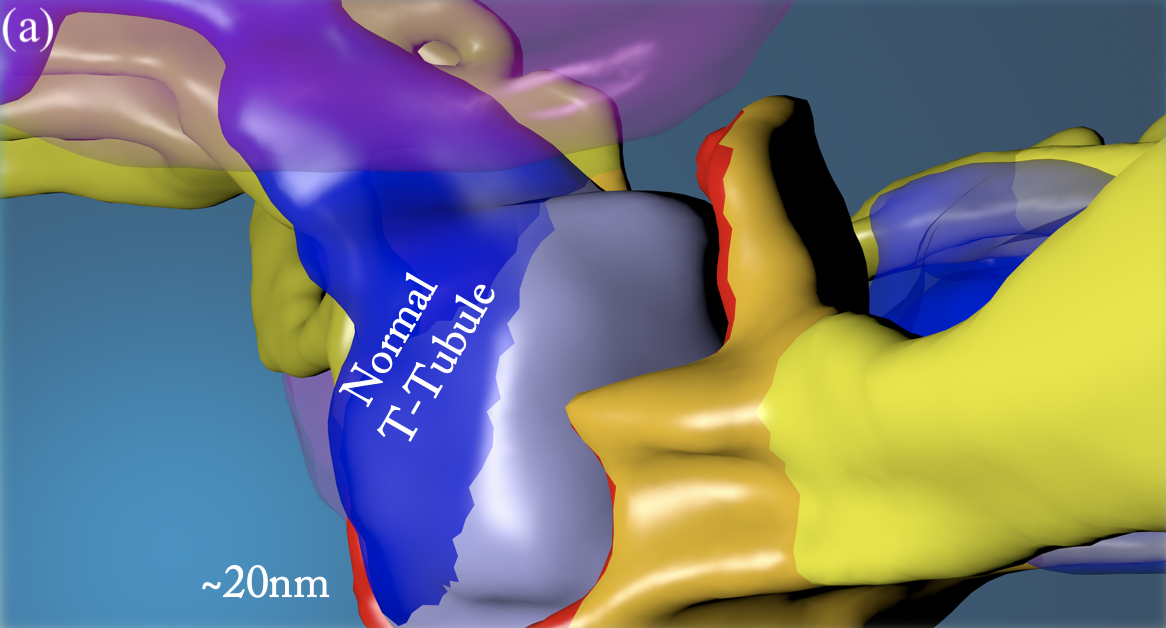
\includegraphics[scale=0.5]{Healthy_geometry.png}
	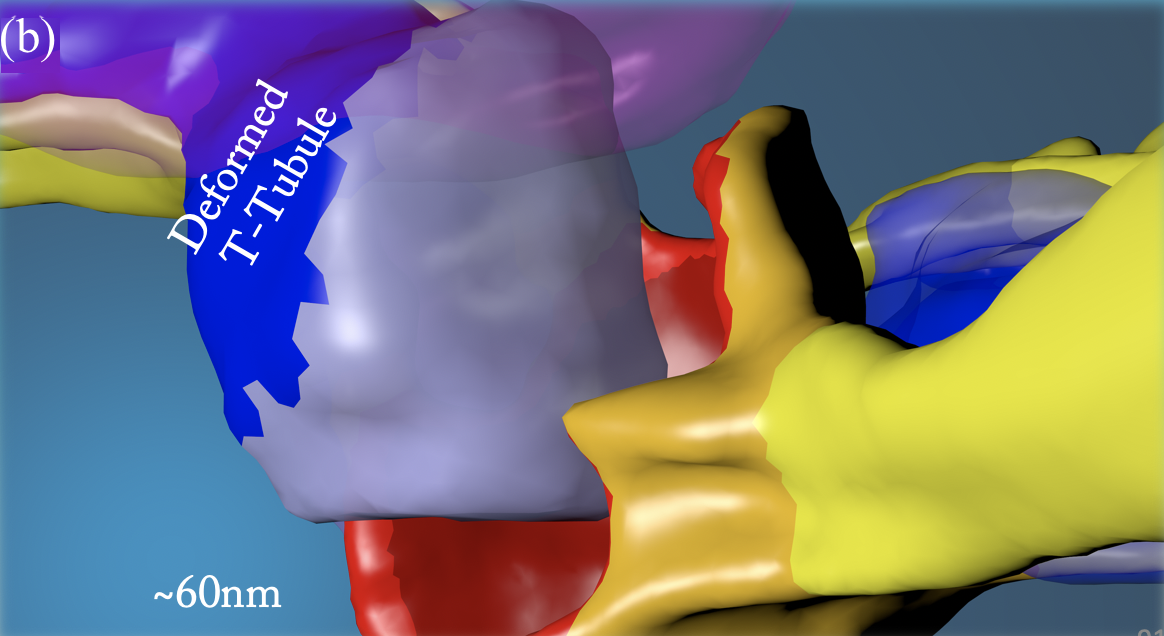
\includegraphics[scale=0.5]{Diseased_geometry.png}
	\caption{Geometries of Normal and Deformed T-Tubules}
	\subcaption{The original, Wild-Type, "Normal" T-Tubule (blue) has an approximate distance of 20nm from the Sarcoplasmic Reticulum; \textbf{(b)} The deformed T-Tubule has a distance of around 60 nm with total displacement of about 40nm from the original position of the T-Tubule}
\label{fig:healthydisease} 
\end{figure}


\begin{comment}

\nocite{Louch2010}
\nocite{Valent2007}
\nocite{Bers2001}%
\nocite{Pitch2011}%
\nocite{Michailova2002}%
\nocite{Fabiato1983}%
\nocite{Robertson1981}%
\nocite{Bondarenko2004}
\nocite{Saftenku2001}%
\nocite{Guo2012}
\nocite{Greenstein2002}
\nocite{Brini2009} %
\nocite{Penheiter2003} %
\nocite{Hilgemann1991}%
\nocite{Higgins2006}%

\end{comment}


\subsection{Cytosolic and SR $Ca^{2+}$ Buffering}

The kinetics for our cytosolic and SR $Ca^{2+}$ buffers were modeled similarly to Hake et al (2012) according to equation 4.1. The cytosolic buffers in our simulations are ATP, Calmodulin (CMDN), Troponin-C (TRPN), and Fluo-4 and our SR buffers are Calsequestrin (CSQN) and Fluo-5. The buffer reaction mechanism is a simple two-step reaction, where the buffer an exist in either apo or $Ca^{2+}$-bound states. 
\begin{equation} 
\ce{B + Ca^2+  <=>[\ce{k_{f}}][\ce{k_{r}}]
$\underset{\text{Calcium-bound Buffer}}{\ce{B \cdot Ca^{2+}}}$
}
\end{equation}

At equilibrium, the product of the forward rate constant, k$_{f}$ and the concentration of $Ca^{2+}$ and the buffer is equal to the product of the concentration of the $Ca^{2+}$-bound buffer and the reverse rate constant, k$_{r}$, according to equation 4.2.  
\begin{equation}
k_{f}[B][Ca^{2+}] = k_{r}[B \cdot Ca^{2+}]
\end{equation}

At equilibrium, the concentration of $Ca^{2+}$ is assumed to be constant. In this way, we can assume a pseudo-first order rate constant, k, equaling to the product of the forward rate constant k$_{f}$ multiplied by the concentration of Calcium (140$\mu$M), according to equation 4.3. 
\begin{equation}
 k = k_{f} \cdot [Ca^2+]
\end{equation}

The pseudo-first order relationship in equation 4.3 can be substituted into equation 4.2, yielding equation 4.4.
\begin{equation}
k[B] = k_{r}[B \cdot Ca^{2+}]
\end{equation}

The above equation can be rearranged to give a ratio of the concentrations of the apo and Calcium-bound buffer state equaling to the ratio of the reverse and pseudo-first order rate constants.
\begin{equation}
\frac{[B]}{[B  \cdot Ca^{2+}]} = \frac{k_{r}}{k} 
\end{equation}

Since the buffer exists in either apo or calcium-bound states, according to equation 4.6, the relationship can be substituted into equation 4.5 solving for the concentration of the apo buffer species in 4.7. 
\begin{equation}
[Total_{B}] = [B] + [B \cdot Ca^{2+}] 
\end{equation}

\begin{equation}
\left[ B\right] = \frac {\left( \frac {k_{r}}{k}\right) \left [Total_{B}\right] }{ 1+\left( \frac {k_{r}}{k}\right) }
\end{equation}

Using this relationship, we are able to solve for the concentration of the buffer species in either apo or $Ca^{2+}$-bound states according to their total concentrations used by Hake et al. The values for the initial concentrations can be found in Table 4.1.
\subsection{Sarcolemmal (T-Tubule) Fluxes}

\subsubsection{PMCA and NCX fluxes}

There are two major sarcolemmal pumps known to maintain homeostasis in cardiomyocytes, the Plasma Membrane Calcium-ATPase (PMCA) pump and the Sodium-Calcium exchanger (NCX) pump \cite{Bers2002}. Hake et al. originally modeled the sarcolemmal pumps using three separate fluxes, PMCA (termed pCa in Hake et al.), NCX, and a background calcium flux, (termed Cab in Hake et al.). In our model, we capture the background calcium flux utilizing "leak" reactions in both our PMCA and NCX models (see figure 4.3a/b). 

\setcounter{figure}{2}
\begin{figure}
\centering
	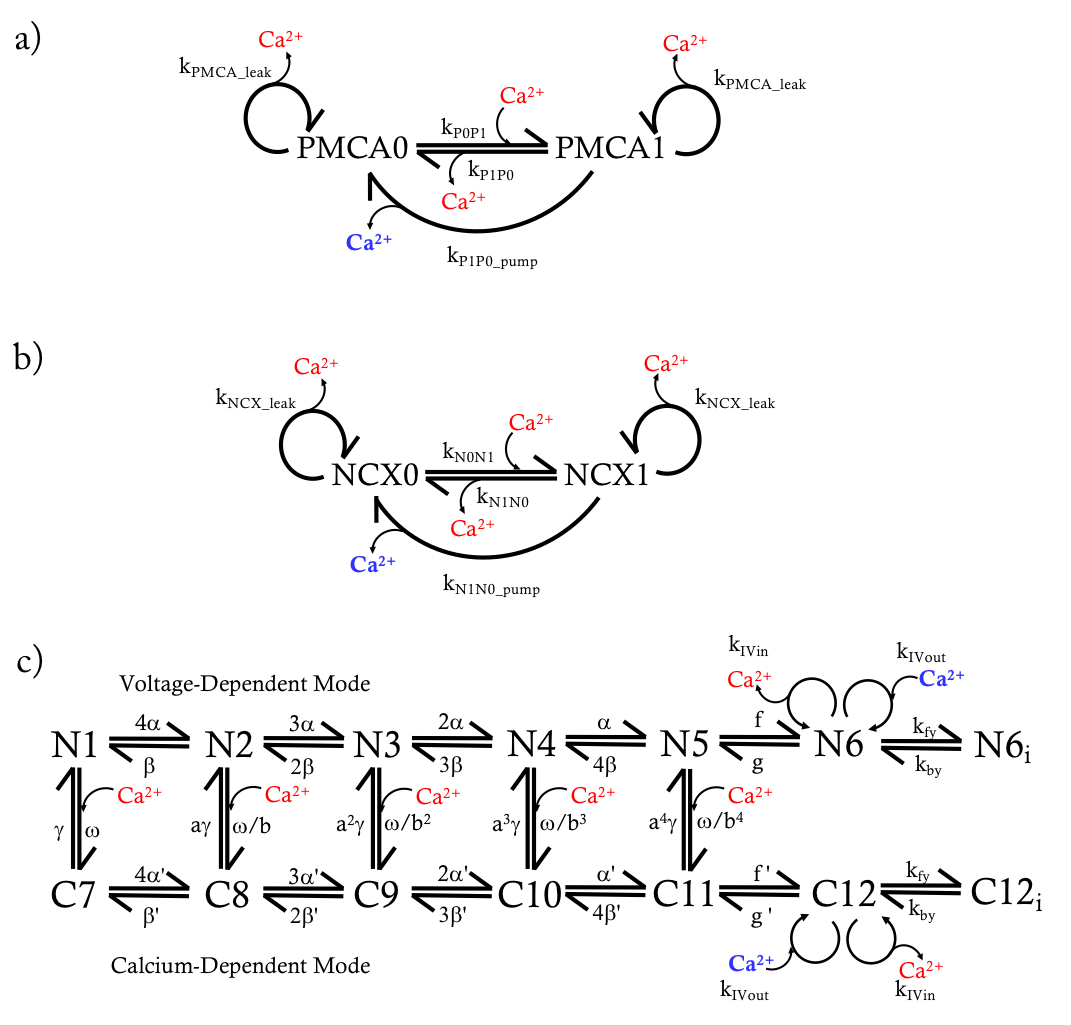
\includegraphics[scale=0.85]{TTfluxes_fig.png}
	\caption{Sarcolemmal (T-Tubule) Fluxes}
	\subcaption{Plasma Membrane Calcium-ATPase Model. Adapted from the model by Bartol et al. (2015) and based on measurements by Brini and Carafoli (2009) and Penheiter et al (2003). Both states are capable of leaking calcium into the cytoplasm (red), corresponding to a background calcium level of 140mM. The transition from state PMCA1 to state PMCA0 pumps one Calcium ion per reaction to the extracellular space (blue). Reaction rate constants can be found in Table 4.2;   \textbf{(b)} Sodium/Calcium Exchanger Model. Adapted from the model by Bartol et al. (2015) and based on measurements by Hilgemann (1991). Both states are capable of leaking calcium into the cytoplasm (red), corresponding to a background calcium level of 140mM.The transition from state NCX1 to state NCX0 pumps one Calcium ion per reaction to the extracellular space (blue). Reaction rate constants can be found in Table 4.2;   \textbf{(c)}Sodium/Calcium Exchanger Model. Adapted from the model by Bartol et al. (2015) and based on measurements by Hilgemann (1991). Both states are capable of leaking calcium into the cytoplasm (red), corresponding to a background calcium level of 140mM.The transition from state NCX1 to state NCX0 pumps one Calcium ion per reaction to the extracellular space (blue). Reaction rate constants can be found in Table 4.2 }
	
\label{fig:TTfluxes} 
\end{figure}

The PMCA pump is modeled as a two-state reaction where one ion of Ca$^{2+}$ can reversibly bind to the first state, and in a seperate, irreversible reaction, calcium is pumped out of the cytosol (see figure 4.3a and equation 4.8). 
\begin{equation}
\ce{PMCA0 + Ca^2+  <=>[\ce{k_{1}}][\ce{k_{-1}}]
$\underset{\text{Calcium-bound Pump}}{\ce{PMCA1}}$
} \ch{ ->[pump] PMCA0}
\end{equation}

The concentration of either state is defined, then, by the total concentration minus the concentration of the other state, according to equation 4.8.

\begin{equation}
\left[PMCA_{1}\right] =\left[PMCA_{Total}\right] - \left[PMCA_{0}\right]
\end{equation}

At equilibrium the concentration of Ca$^{2+}$ is constant, and thus, a pseudo-first order rate constant, k$_{f}$, can be assumed, as in equation 4.10. 

\begin{equation}
k_{f} = [Ca^{2+}] \cdot k_{1}
\end{equation}

The rate of change of a state, for example, PMCA$_{0}$, can be written as the equation in 4.11, which is simply the sum of the PMCA$_{0}$ producing reactions minus the PMCA$_{0}$ consuming reactions.
\begin{equation}
\frac{d\left[PMCA_{0}\right]}{dt} = \left[PMCA_{1}\right]k_{-1} + \left[PMCA_{1}\right] k_{pump} - \left[PMCA_{0}\right] k_{f}
\end{equation}

At equilibrium, the rate of change is zero, and can be used to solve for the concentration of one of the two states as in equations 4.12-4.15.
\begin{equation}
0 = \frac{d\left[PMCA_{0}\right]}{dt}
\end{equation}

\begin{equation}
0 = (k_{-1}-k_{pump}) (\left[PMCA_{Total}\right] - \left[PMCA_{0}\right])- \left[PMCA_{0}\right] k_{f}
\end{equation}

\begin{equation}
0 = \left[PMCA_{Total}\right] (k_{-1} + k_{pump}) - \left[PMCA_{0}\right](k_{-1} + k_{pump}) - \left[PMCA_{0}\right] k_{f}
\end{equation}

\begin{equation}
\left[PMCA_{0}\right] = \frac{\left[PMCA_{Total}\right] (k_{-1} + k_{pump}) - \left[PMCA_{0}\right](k_{-1} + k_{pump})}{k_{f}}
\end{equation}

To account for the background $Ca^{2+}$ level that maintains an equilibrium of 140$\mu$M, each state of the pump was assigned to a leak rate which is defined as the ratio of the product of the forward pump rate constants over all the produce of the total rate constants. 

\begin{equation}
k_{leak} = \frac{k_{pump} \cdot k_{f}}{k_{f}+ k_{-1}+ k_{pump}}
\end{equation}


In this way, we can solve for the steady state concentrations of PMCA in either state. The same relationships were used to model the NCX pump, but are not shown in the interest of brevity. 


\subsubsection{L-Type Calcium Channel flux}

\setcounter{figure}{3}
\begin{figure}
\centering
	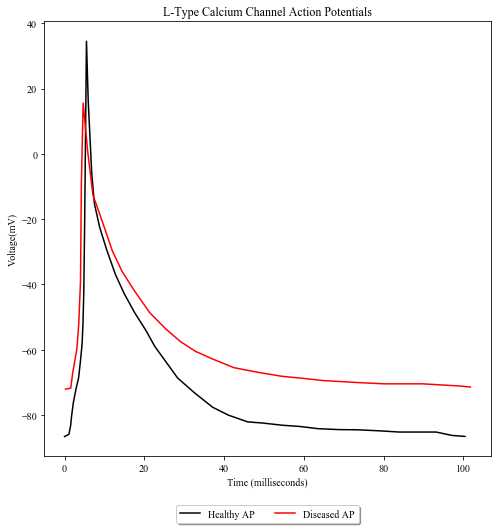
\includegraphics[scale=0.5]{ap.png}
	\caption{L-Type Calcium Channel Action Potentials}Healthy (black) and Diseased (red) action potentials used to stimulate the LTCC, based on the model by Morotto et al (2014).
\end{figure}

In an effort to further improve upon the the original Calcium Release Unit mode, we aimed to model a \textit{triggered} $Ca^{2+}$ spark, or the process known as Calcium-Induced Calcium Release. In order to do this, we included a model of the voltage-dependent Calcium Channel, known as the L-Type Calcium Channel (LTCC). We adapted the model of LTCC dynamics developed by Greenstein and Winslow \cite{Greenstein2002} to be used in our system. We used two different action potentials to stimulatie our LTCC 1) "healthy" or WT and 2) "diseased" or Calmodulin-Dependent Kinase II over-expression (CaMKII-OE) action potentials as modelled by Morotti et al. \cite{Morotti2014} (see figure 4.4). The LTCC model has both voltage-dependent modes and Calcium-dependednt modes. Using this LTCC model we were able to model the rate constants of LTCC state transitions as a function of membrane calcium reactions, voltage and time, according to the relationships described by Greenstein and Winslow (see figure 4.3c), described below.

The forward rate constants of the voltage-dependent modes, $\alpha$ are a function of the membrane voltage, according to equation 4.17. 
\begin{equation}
\alpha = 2.0 e ^ { 0.012 \left( \mathrm { V } _ { \mathrm { m } } - 35 \right) }
\end{equation}

The reverse rate constants of the voltage-dependent modes, $\beta$ are a function of the membrane voltage, according to equation 4.18. 
\begin{equation}
\beta = 0.0882 e ^ { - 0.05 \left( \mathrm { V } _ { \mathrm { m } } - 35 \right) }
\end{equation}

The forward rate constants of the calcium-dependent modes, $\alpha ^ { \prime }$ are a scalar multiple of $\alpha$ given by equation 4.19. 
\begin{equation}
\alpha ^ { \prime } = a \alpha
\end{equation}

The reverse rate constants of the calcium-dependent modes, $\beta ^ { \prime }$ are a scalar multiple of $\beta$ given by equation 4.20. 
\begin{equation}
\beta ^ { \prime } = b \beta
\end{equation}

The parameters defining the forward rate constant, $k_{ fy }$, and reverse rate constant, $k_{ ry }$, of the voltage and calcium-dependent inactivation are defined by equations 4.21 through 4.24.

\begin{equation}
y _ { \infty } = 0.4 / \left( 1 + e ^ { \left( \mathrm { V } _ { \mathrm { m } } + 12.5 \right) / 5 } \right) + 0.6
\end{equation}

\begin{equation}
\tau _ { \mathrm { y } } = 340 / \left( 1 + e ^ { \left( \mathrm { V } _ { \mathrm { m } } + 30 \right) / 12 } \right) + 60
\end{equation}

\begin{equation}
k _ { \mathrm { f } , \mathrm { y } } = y _ { \infty } / \tau _ { \mathrm { y } }
\end{equation}

\begin{equation}
k _ { \mathrm { b } , \mathrm { y } } = \left( 1 - y _ { \infty } \right) / \tau _ { \mathrm { y } }
\end{equation}


In order to calculate the inward flux of calcium through the LTCC k$_{IVin}$ and the outward flux k$_{IVout}$, we  converted the permeability of Ca$^{2+}$ P$_{Ca}$ to units ions/sec using equation 4.25 and 4.26. We assume 2mM extracellular calcium concentration. We use the following two equations where $N_{A}$ is Avogadro's number, \textit{z} is charge/ion,  V$_{m}$ is the membrane voltage and \textit{F} is Faraday's constant, R is the universal gas constant, and T is temperature (see table 4.3).


\begin{equation}
 k_{IVin} =\frac {[Ca^{2+}] \frac{N_{A}}{z} P_{Ca}4V_{m}F0.341}{RTe^{\frac {2V_{m}F}{RT}-1}}
\end{equation}


\begin{equation}
 k_{IVout} =\frac {\frac{N_{A}}{z} P_{Ca}4V_{m}Fe^{\frac {2V_{m}F}{RT}}}{RTe^{\frac {2V_{m}F}{RT}-1}}
\end{equation}


\subsection{Sarcoplasmic Reticulum Fluxes}
\subsubsection{Sarco/Endoplasmic Reticulum Calcium-ATPase (SERCA) pump kinetics}

\setcounter{figure}{4}
\begin{figure}
\centering
	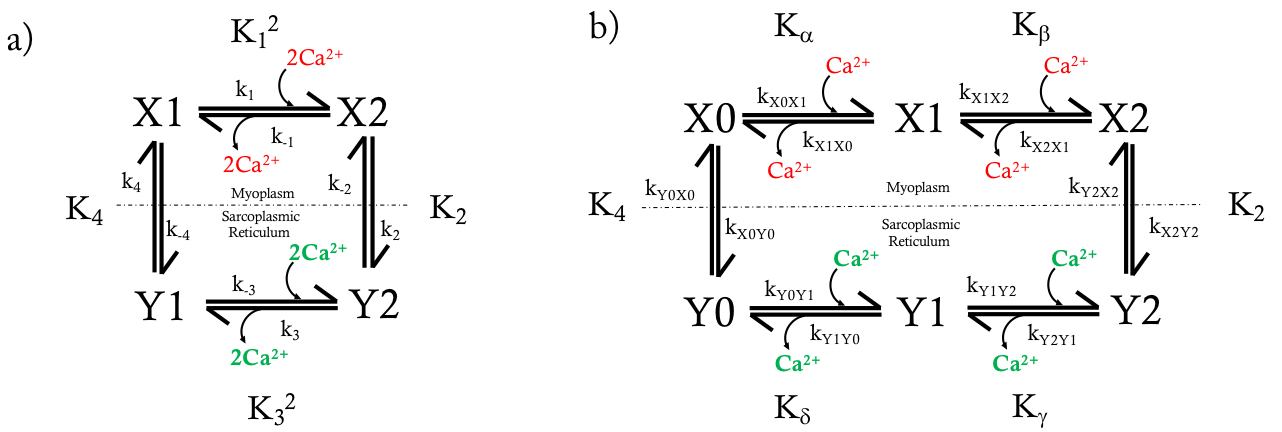
\includegraphics[scale=0.73]{SERCA2_fig.png}
	\caption{SERCA Models}
	\subcaption{Sarco/Endoplasmic Reticulum Calcium-ATPase (SERCA) Model by Higgins et al. Two cytoplasmic-facing states (X) and two sarcoplasmic reticulum-facing states (Y) translocate cytosolic Calcium (red) to the sarcoplasmic reticulum (green).}
	\subcaption{Sarco/Endoplasmic Reticulum Model. Adapted from the model by Higgins et al 2006 by separating the event of two $Ca^{2+}$ binding/unbinding into individual $Ca^{2+}$ binding/unbinding reactions. Three cytoplasmic-facing states (X) and three sarcoplasmic reticulum-facing states (Y) translocate cytosolic Calcium (red) to the sarcoplasmic reticulum (green). Reaction rate constants can be found in Table 4.5 }
\label{fig:SERCAHiggins} 
\end{figure}


 Of utmost importance in the dynamics of $Ca^{2+}$ during the phenomenon of CICR is the action of the SERCA pump, which is estimated to be responsible for the clearing of 70-90\% of cardiomyocyte $Ca^{2+}$ after a release event event \cite{Bers2002}. In a single forward cycle of the SERCA pump, one molecule of ATP is consumed to translocate two ions of $Ca^{2+}$ from the cytoplasm into the SR, the intracellular $Ca^{2+}$ store.  In order to explicitly model the dynamics of $Ca^{2+}$ in the myoplasm and inside the SR, it is necessary to use models that treat calcium as individual species. In order to achieve this, we adapted a model of SERCA by Higgins et al. \cite{Higgins2006} as modeled in our previous work \cite{Bartol2015} to reproduce the dynamics of SERCA2a, maintaining 140nM cytoplasmic $Ca^{2+}$ while satisfying microscopic reversibility. 

The four-state model by Higgins et al. \cite{Higgins2006} (Figure 4.5) groups both $Ca^{2+}$ binding and unbinding events into a single step (see Figure 4.5,a) $K_{1}$ and $K_{3}$, respectively). In our adapted version of the Higgins model, we model SERCA as a six-state pump that binds (see Figure 4.5,b) $K_{\alpha}$ and $K_{B}$) and unbinds (see figure 4.3,b) $K_{\gamma}$ and $K_{\delta}$) $Ca^{2+}$ ions discretely. In order to accomplish this, the equilibrium constants for binding and unbinding $Ca^{2+}$  ($K_{1}$ and $K_{3}$, respectively) needed to be split up into two equilibrium constants for the individual binding ($K_{\alpha}$ and $K_{\beta}$) and unbinding ($K_{\gamma}$ and $K_{\delta}$) events. This was accomplished using the theory of ligand occupancy developed by Sine and Taylor \cite{Sine1979,Sine1980,Sine1981}. 

Firstly, we assume that the $Ca^{2+}$  equilibrium constant for the binding of 2 $Ca^{2+}$ ions, $K_{1}^{2}$ is the product of the individual equilibrium constants, $K_{\alpha}$ and $K_{\beta}$, according to equations 4.27-4.30, below. 
\begin{equation}
K_{1}^{2}= K_{\alpha} \times K_{\beta}
\end{equation}

\begin{equation}
K_{\alpha} = \frac{k_{X1X0}}{k_{X0X1}} 
\end{equation}

\begin{equation}
K_{\beta} = \frac{k_{X2X1}}{k_{X1X2}}
\end{equation}

\begin{equation}
K^{2}_{1}=  \frac{k_{X1X0}}{k_{X0X1}} \times \frac{k_{X2X1}}{k_{X1X2}}
\end{equation}

Because there are two sites to which  $Ca^{2+}$ can bind in state X0 and only one state to which  $Ca^{2+}$ can bind to in state X1, the relationship of the $Ca^{2+}$ binding rate constants in equation 4.31 is assumed. 

\begin{equation}
k_{X0X1}=2 \times k_{X1X2} 
\end{equation}

Likewise and in the same way, there are two sites from which  $Ca^{2+}$ can unbind in state X2 and only one site to which $Ca^{2+}$ can unbind to in state X1. And so, the relationship of the $Ca^{2+}$ unbinding rate constants in equation 4.32 is assumed. 

\begin{equation}
k_{X2X1}=2 \times k_{X1X0} 
\end{equation} 

Substituting into equation 4.30 for the rate constant relationships 4.31 and 4.32, yields equation 4.34.

\begin{equation}
K^{2}_{1}=  \frac{k_{X1X0}}{2 \times k_{X1X2}} \times \frac{2 \times k_{X1X0}}{k_{X1X2}} = \left(\frac{k_{X1X0}}{k_{X1X2}}\right)^{2}
\end{equation}

According to the relationship of the equilibrium constants in equations 4.31-32, the relationship between the equilibrium constants $K_{\alpha}$ and $K_{\beta}$ is the one given by equation 4.34.

\begin{equation}
K_{\alpha}= \frac{K_{\beta}}{4}
\end{equation}

We solve for the individual rate constants by substituting the relationship given in 4.34 into equation 4.35 yielding equations 4.36-38. 


\begin{equation}
K_{1}= \sqrt{K_{\alpha} \times K_{\beta}}
\end{equation}


\begin{equation}
K_{1}= \sqrt{ \frac{K_{\beta}^2}{4}}
\end{equation}

\begin{equation}
K_{\alpha}= \frac{K_{1}}{2} 
\end{equation}

\begin{equation}
K_{\beta}= K_{1} \times 2
\end{equation}



In the same way, we can derive the individual rate constants, $K_{\gamma}$ and $K_{\delta}$ from the equilibrium constant for the unbinding of 2 $Ca^{2+}$ ions, $K_{3}^{2}$.  

\begin{equation}
K_{3}^{2}= K_{\gamma} \times K_{\delta}
\end{equation}

\begin{equation}
K_{\gamma} = \frac{k_{Y1Y2}}{k_{Y2Y1}} 
\end{equation}

\begin{equation}
K_{\delta} = \frac{k_{Y0Y1}}{k_{Y1Y0}}
\end{equation}

\begin{equation}
K^{2}_{3}=   \frac{k_{Y1Y2}}{k_{Y2Y1}} \times \frac{k_{Y0Y1}}{k_{Y1Y0}}
\end{equation}

There are two sites to which  $Ca^{2+}$ can unbind from in state Y2 and only one state from which $Ca^{2+}$ can unbind state Y1. Thus, the relationship between $Ca^{2+}$ unbinding rate constants in equation 4.43 is assumed. 

\begin{equation}
k_{Y1Y0}=2 \times k_{Y2Y1} 
\end{equation}

There are two sites to which $Ca^{2+}$ can bind in state Y0 and only one site to which $Ca^{2+}$ can bind to in state Y1. As such, the relationship of the $Ca^{2+}$ binding rate constants in equation 4.44 is assumed. 


\begin{equation}
k_{Y0Y1}=2 \times k_{Y1Y2} 
\end{equation} 

Substituting into equation 4.42 for the rate constant relationships 4.43 and 4.44, yields equation 4.45.

\begin{equation}
K^{2}_{3}=  \frac{k_{Y1Y2}}{2 \times k_{Y1Y0}} \times \frac{2 \times k_{Y1Y2}}{k_{Y1Y0}} = \left(\frac{k_{Y1Y2}}{k_{Y1Y0}}\right)^{2}
\end{equation}

According to the relationship of the equilibrium constants in equations 4.43 and 4.44, the relationship between the rate constants $K_{\gamma}$ and $K_{\delta}$ is the one given by equation 4.46.

\begin{equation}
K_{\delta}= \frac{K_{\gamma}}{4}
\end{equation}

We solve for the individual rate constants by substituting the relationship given in 4.46 into equation 4.47 yielding equations 4.48-4.50. 


\begin{equation}
K_{3}= \sqrt{K_{\gamma} \times K_{\delta}}
\end{equation}


\begin{equation}
K_{3}= \sqrt{\frac{K_{\gamma}^2}{4}}
\end{equation}

\begin{equation}
K_{\gamma}= K_{3} \times 2
\end{equation}

\begin{equation}
K_{\delta}= \frac{K_{3}}{2} 
\end{equation}

According to Higgins et al., the relationship between the Gibbs Free energy of 1 molecule of ATP and the kinetic cycle is given by equation 4.51.
\begin{equation}
K _ { 1 } ^ { 2 }   K _ { 2 } K _ { 3 } ^ { 2 } K _ { 4 } = e ^ { \Delta \mathrm { G } _ { \mathrm { ATP } } ^ { 0 } / \mathrm { RT } }
\end{equation}

Using the rate constants described in Table 4.5 and the relationships described above, yields a Gibbs free energy of -47.0943 kJ/mol. The product of the forward rates constants equals the product of the reverse rate constants. At steady state, this is also true for the product of the forward reaction rates and the product of the reverse reaction rates, satisfying detailed balance. Lastly, the pump reaches steady state at a cytosolic concentration, $Ca^{2+}_{ \mathrm { cyt } _ { \mathrm { ss } } }$, of 140nM and a SR concentration, $Ca^{2+} _ { \mathrm { sr } _ { \mathrm { ss } } } $, of 1.3mM.

\begin{equation}
Ca^{2+} _ { \mathrm { sr } _ { \mathrm { ss } } } = \frac {Ca^{2+}_{ \mathrm { cyt } _ { \mathrm { ss } } } } { K _ { 1 } K _ { 3 } \sqrt { K _ { 2 } K _ { 4 } } }
\end{equation}

\setcounter{figure}{5}
\begin{figure}
\centering
	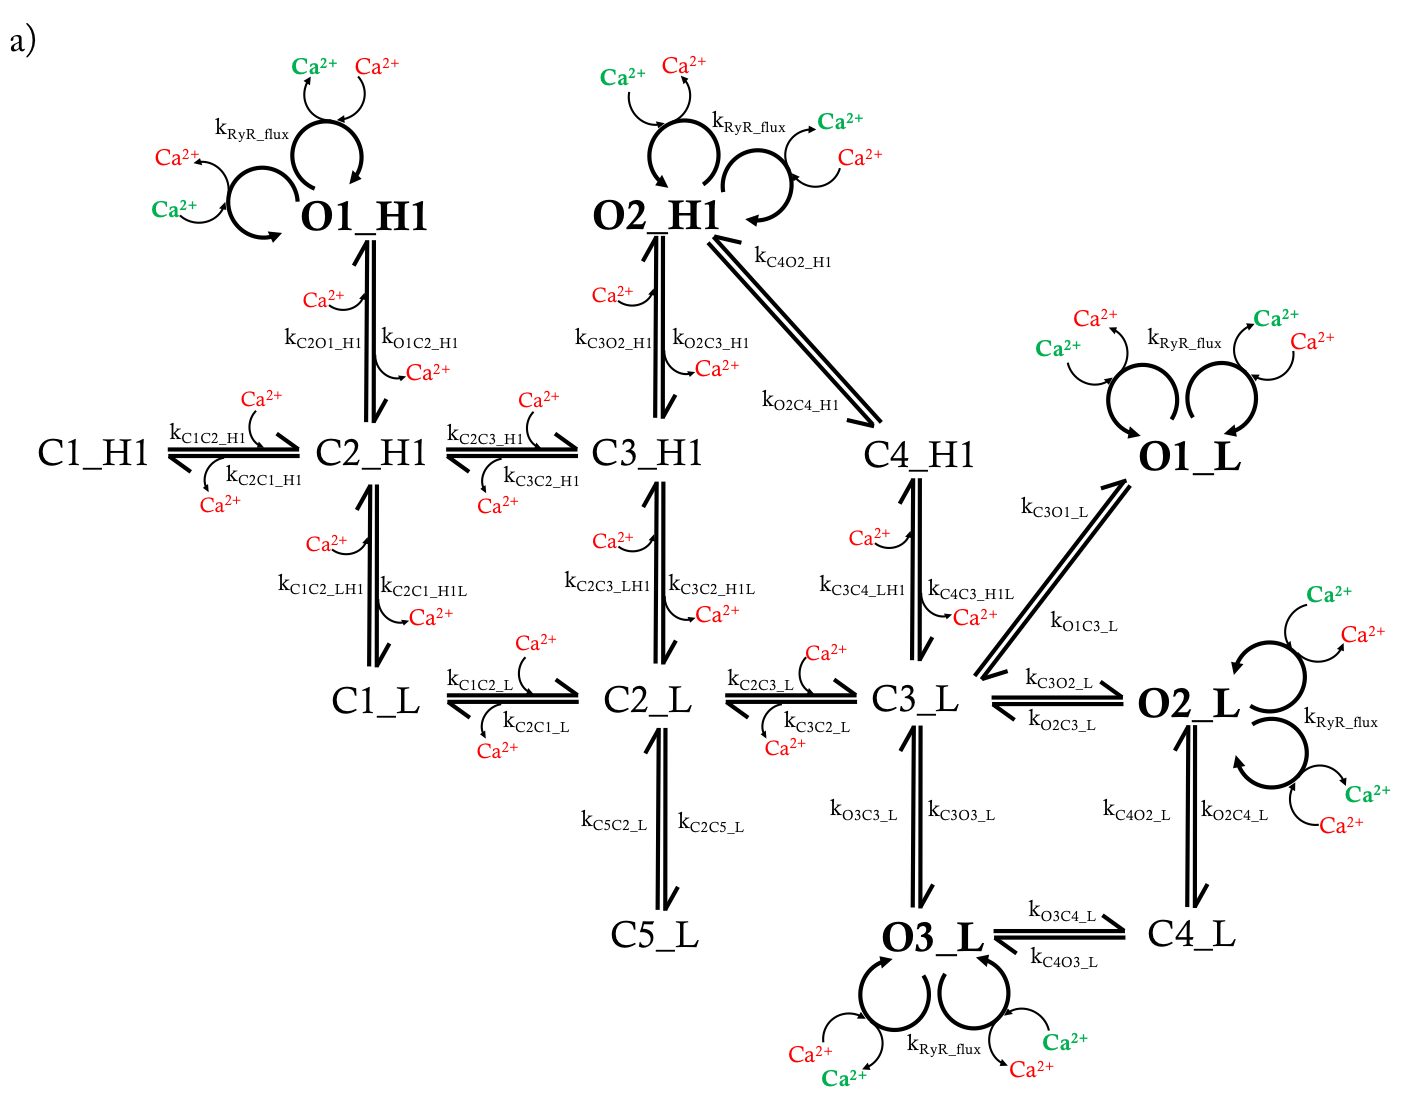
\includegraphics[scale=0.6]{RyRflux_fig.png}	
	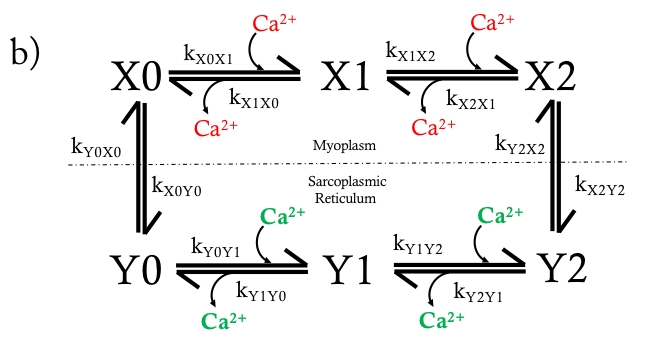
\includegraphics[scale=0.6]{SERCAflux_fig.png}
	\caption{Sarcoplasmic Reticulum Fluxes}
	\subcaption{Ryanodine Receptor Markov Model. Adapted from the Markov Model by Saftenku et al. (2001); Nine closed (C) states and five open (O) states describe the kinetic scheme of the Ryanodine Receptor. Cytosolic Calcium (Red) binds to closed states in High (H1) and Low (L) gating modes. In open states, Sarcoplasmic Reticulum Calcium (Green) and Cytosolic Calcium are translocated through the receptors. Reaction rates can be found in Table 4.4.}
	\subcaption{Sarco/Endoplasmic Reticulum Model. Adapted from the model by Higgins et al 2006. Three cytoplasmic-facing states (X) and three sarcoplasmic reticulum-facing states (Y) translocate cytosolic Calcium (red) to Calcium the sarcoplasmic reticulum (green). Reaction rate constants can be found in Table 4.5}
\label{fig:SRfluxes} 
\end{figure}

\subsubsection{Ryanodine Receptor (RyR) kinetics}

In order to simulate a triggered Ca$^{2+}$ spark, it was necessary to model the complexities of the Sarcoplasmic Reticulum Ca$^{2+}$ release channel, the Ryanodine Receptor. Hake's original simulations used a simplistic, binary model of RyR that could exist in either an open or a closed state. Once a certain voltage was sensed, the RyR would close and never re-open. Most notably the RyR in these simulations did not activate in response to an action potential stimulus or change in dyadic Ca$^{2+}$ levels, but instead were set to "open" to initiate the spark. RyR is known to interact with 30+ binding partners \cite{Song2011}, and thus, can exist in a multitude of states. In an attempt model this complexity, we incorporated a Markov model of RyR that captures its low and high gating modes as well as its ability to bind Ca$^{2+}$ as a basis for its activation.

We adapted the Markov model of RyR dynamics by Saftenku et al. \cite{Saftenku2001} for use in MCell simulations (see Figure 4.6a). Coincidentally, this was the same model of RyR used by Koh et al in their MCell simulations using simplistic geometries\cite{Koh2006}. 

The parameters for the RyR model (see Table 4.4) were used with little adaptation with the exception of the RyR flux. For the purpose of our simulations, the RyR flux had to be converted to units of Ca$^{2+}$ ions/second. This was accomplished using the single-channel current, measured at 0.35 pA at 1mM by Guo et al \cite{Guo2012} and the relationship described in equation 4.53, below.

\begin{equation}
k_{RyRflux} = \frac {I^{RyR}6.242\times 10^{18}\frac{Charge}{Coulomb}}{\left[ Ca^{2+}\right] z} = \frac{9.01\times10^{-9}  Ca^{2+}ions}{s}
\end{equation}

Amps are defined as units of $\frac{Coulomb}{second}$. Thus, the RyR current, $I^{RyR}$ in pA can be converted to charges by multiplying the conversion factor, $6.242\times 10^{18}\frac{Charge}{Coulomb}$. Using the 1mM concentration of Calcium and a charge or, \textit{z}, value of 2, equals to a rate constant of $ 9.01\times10^{-9}\frac{ Ca^{2+}ions}{s}$.
%Reversal potential -2.4mV and Voltage of ER = 0mV





\begin{comment}

\begin{equation}
\lambda=\sqrt {4D\Delta t}
\label{eq:dimensionless radial distance}
\end{equation}

\begin{equation}
\tilde{r}={\frac{r}{\lambda}}
\label{eq:dimensionless radial distance}
\end{equation}

\begin{equation}
\overline {l}_{\bot}=\sqrt {\frac {4D\Delta t}{\pi }}
\label{eq:Orthogonal step length}
\end{equation}


\begin{equation}
\overline {l}_{r}=\overline {l}_{\bot}\times 2
\label{eq:radial diffusional step length}
\end{equation}


\begin{equation}
{N}_{H}={N}_{\si{\angstrom}}\overline {l}_{\bot}{A}_{ET}{[A]}_{o}
\label{eq:Orthogonal step length}
\end{equation}



Where ${[A]}_{o}$ is the initial concentration of the species, ${A}_{ET}$ is the area of the effector tile, $\overline {l}_{\bot}$ is the average orthogonal step length, ${N}_{\si{\angstrom}}$ is Avogadro's number and ${N}_{H}$ is the number of hits.




\begin{equation}
[ \mathrm { ATP } ] _ { \mathrm { tot } } = [ \mathrm { ATP } ] _ { \mathrm { tot } - \mathrm { i } } = [ \mathrm { ATP } ] _ { \mathrm { tot } - \mathrm { ss } }
\end{equation}

\begin{equation}
[ \mathrm { ATP } ] _ { \mathrm { ss } } = [ \mathrm { ATP } ] _ { \mathrm { tot } } - [ \mathrm { CaATP } ] _ { \mathrm { ss } } - [ \mathrm { MgATP } ] _ { \mathrm { ss } }
\end{equation}

\begin{equation}
\left[ ATP\right]_{ss} = \frac{k^{MgATP}_{r}\left[ MgATP\right] _{ss}+J^{MgATP}_{xfer}\dfrac {V_{myo}}{V_{ss}}}{k^{MgATP}_{f}\left[ Mg\right] _{SS}}
\end{equation}


\begin{equation}
\begin{aligned} \frac { \mathrm { d } [ \mathrm { CaATP } ] _ { \mathrm { ss } } } { \mathrm { d } t } = & - J _ { \mathrm { xfer } } ^ { \mathrm { CaATP } } \frac { V _ { \mathrm { myo } } } { V _ { \mathrm { ss } } } + k _ {f} ^ { \mathrm { CaATP } } [ \mathrm { Ca } ] _ { \mathrm { ss } } [ \mathrm { ATP } ] _ { \mathrm {ss} } -k _ {r} ^ { \mathrm { CaATP } } [ \mathrm { CaATP } ] _ { \mathrm { ss } } \end{aligned}
\end{equation}


\begin{equation}
\frac{d\left[CaATP\right]_{ss}}{dt} = 0
\end{equation}

\begin{equation}
\left[ CaATP\right] _{ss}=-\frac {J^{CaATP}_{xfer}\dfrac {V_{myo}}{V_{ss}}+k^{CaATP}_{f}\left[ Ca\right] _{ss}\left[ ATP\right] _{ss}}{k^{CaATP}_{r}}
\end{equation}


\begin{equation}
\begin{aligned} \frac { \mathrm { d } [ \mathrm { MgATP } ] _ { \mathrm { ss } } } { \mathrm { d } t } = & - J _ { \mathrm { xfer } } ^ { \mathrm {MgATP } } \frac { V _ { \mathrm { myo } } } { V _ { \mathrm { ss } } } + k _ {f} ^ { \mathrm { MgATP } } [ \mathrm { Mg } ] _ { \mathrm { ss } } [ \mathrm { ATP } ] _ { \mathrm {ss} } -k _ {r} ^ { \mathrm {MgATP } } [ \mathrm { MgATP } ] _ { \mathrm { ss } } \end{aligned}
\end{equation}


\begin{equation}
\frac{d\left[MgATP\right]_{ss}}{dt} = 0
\end{equation}

\begin{equation}
\left[ MgATP\right] _{ss}=-\frac {J^{MgATP}_{xfer}\dfrac {V_{myo}}{V_{ss}}+k^{MgATP}_{f}\left[ Mg\right] _{ss}\left[ ATP\right] _{ss}}{k^{MgATP}_{r}}
\end{equation}

\end{comment}


 \section{Results and Discussion}

\subsection{Buffer and Fluorophore Dynamics}
We began our investigations by building the model from a baseline, using cytosolic buffers, sarcolemmal pumps, and fluorophores as the subjects of our simulations. To make sure equilibrium is maintained in our simulations, we investigated the dynamics of Calcium and its buffers in simulations lacking the sarcollemal stimulus, L-Type Calcium Channel. Because Ryanodine receptors are known to spontaneously activate in the presence of Calcium\cite{Cheng1993,Cannell1995}, and SERCA itself is known to act as a buffer\cite{Higgins2006} we sought to eliminate these effects to establish that our "baseline system," comprised of cytosloic and SR buffers and fluorophores, maintains equilibrium. A question addressed by Hake et al. in their original investigation centered on the effect of fluorophores in the simulations. We also decided to test this effect in our initial simulations. 

The system dynamics comparing the effects of the fluorophores on the baseline system (containing only buffers and sarcollemal pumps) are nearly identical (see Figure 4.7). The most pronounced effect is on the cytosolic buffer, Troponin C (See Figure 4.7e) which differs, on average, only 14 molecules between simulations with and without fluorophores. Due to a high concentration of TRPN and TRPN-Ca$^{2+}$ in the simulations (70 $\mu$M total, 13.2 $\mu$M bound to Calcium, 56.8 $\mu$M free), this corresponds to a difference of 0.036\% on average between the two systems, which is arguably negligible. 

\setcounter{figure}{6}
\begin{figure}
\centering
	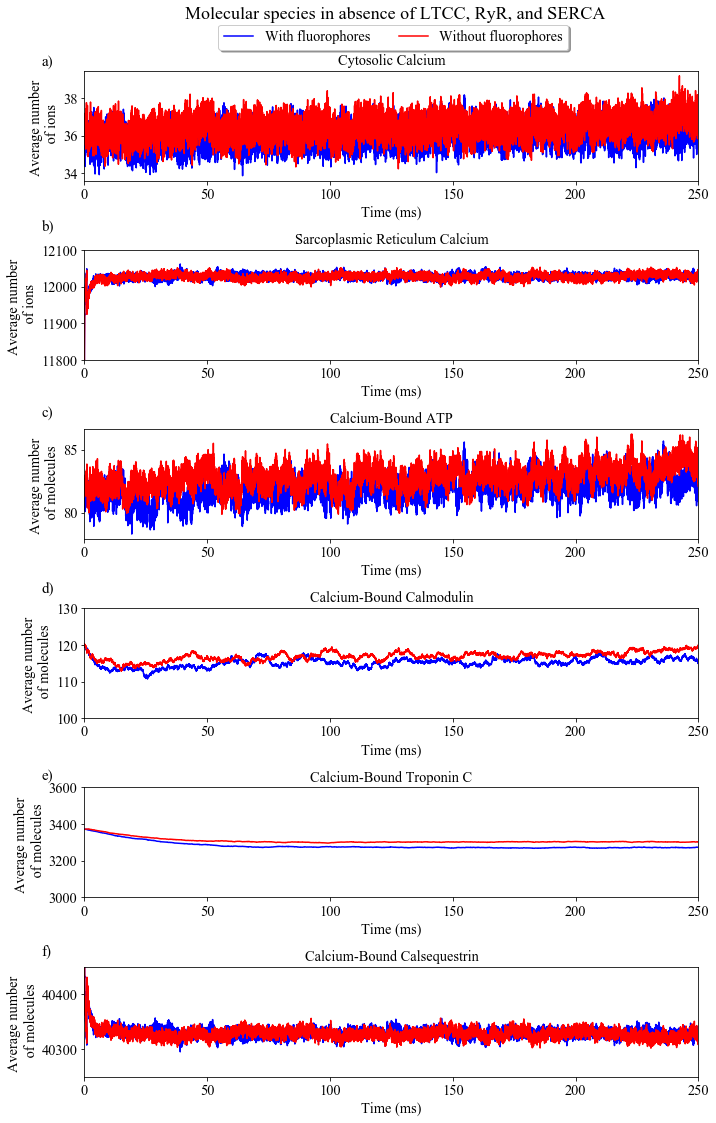
\includegraphics[scale=0.45]{buffer_fluo_molecules_c_Comparison.png}
	\caption{Molecular species in absence of LTCC, RyR and SERCA} 
	\subcaption{Cytosolic Calcium dynamics; \textbf{(b)} Sarcoplasmic Reticulum Calcium dynamics; \textbf{(c)} Calcium-bound ATP; \textbf{(d)} Calcium-bound Calmodulin; \textbf{(e)} Calcium-bound Troponin-C; \textbf{(f)} Calcium-bound Calsequestrin; Comparing simulations with only RyR (blue) and RyR and SERCA(red)}
\label{fig:buffer_fluo} 
\end{figure}

\subsection{Ryanodine Receptor activation profiles} 

\subsubsection{Spontaneous calcium sparks in absence of LTCC}

In order to validate our model, we sought confirmation that that our system could generate spontaneous Ca$^{2+}$ sparks without an LTCC stimulus as observed in experiments \cite{Cheng1993,Lopez-Lopez1994,Cannell1995}. In order to test this, we simulated our CRU system in absence of an action potential stimulus but in the presence of RyR with and without SERCA (see Figure 4.8). Though the average of total number of RyR openings (n=128) are low, there is a non-zero probability that RyR in be triggered spontaneously.

\setcounter{figure}{7}
\begin{figure}
%\centering
	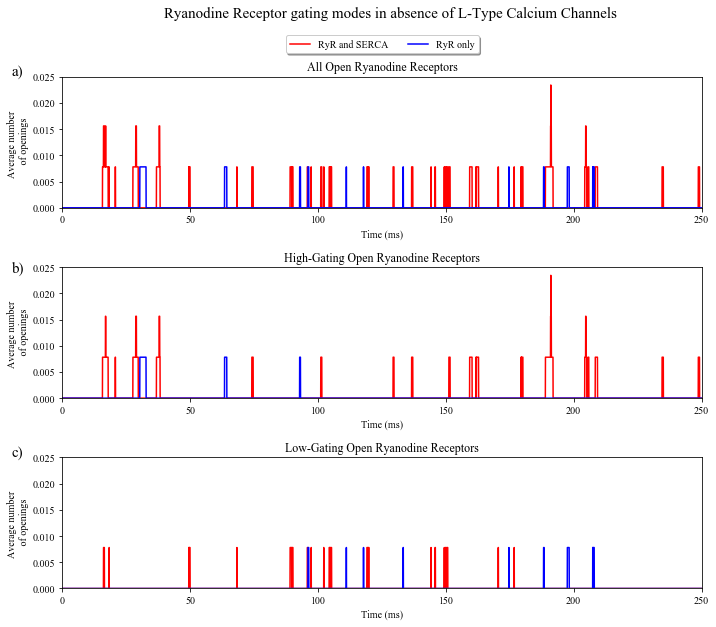
\includegraphics[scale=0.6]{buffer_fluo_RyR_r_Comparison.png}
	\caption{Ryanodine Receptor gating modes in absence of L-Type Calcium Channels} 
	\subcaption{All open Ryanodine Receptors; \textbf{(b)} High-gating open Ryanodine Receptors; \textbf{(c)} Low-gating open Ryanodine Receptors; RyR and SERCA (red) and only RyR (blue)}
\label{fig:Buffer RyR} 
\end{figure}

\subsubsection{Triggered calcium sparks: RyR response to LTCC alterations}
Having established that RyR are capable of firing spontaneously in the absence of an AP stimulus, we sought to confirm that a single LTCC could activate RyRs as previously demonstrated by Sobie et al\cite{Sobie2002}. Figure 4.9 demonstrates that one LTCC with a single action potential is sufficient to activate RyR. 

\setcounter{figure}{8}
\begin{figure}
%\centering
	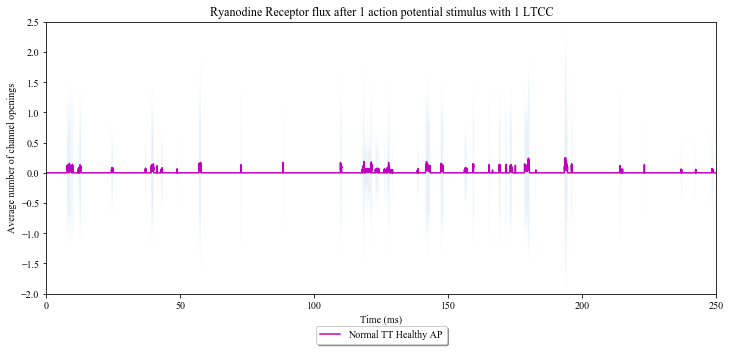
\includegraphics[scale=0.55]{RyRflux_1AP_1LTCC.png}
	\caption{Ryanodine Receptor flux after a single action potential stimulus with a single L-Type Calcium Channel} Average number of openings of RyR in normal T-Tubules simulated with a single L-Type Calcium Channel and the healthy action potential (purple). Standard deviations are shown in light blue.
\label{fig:RyR flux 1 LTCC} 
\end{figure}

Following our simulations with 1 LTCC, we sought to understand the effect that increasing the number of LTCC would have on triggered Calcium release. We comparatively investigated CICR with 1, 2, 4, 6, 8, and 10 LTCC. We predicted that increasing LTCC would result in increased gain, or SR Ca$^{2+}$ efflux through RyR. Consistent with experimental findings, \cite{Cannell1995} increasing the LTCC results in positive gain as demonstrated in figure 4.10.

\setcounter{figure}{9}
\begin{figure}
%\centering
	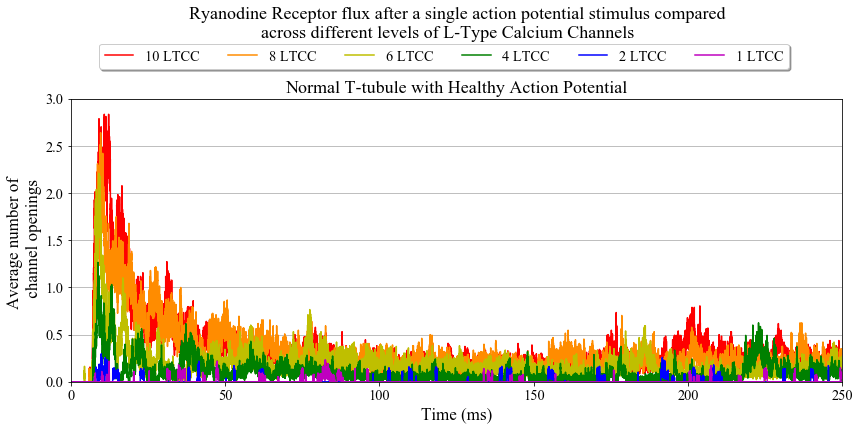
\includegraphics[scale=0.5]{RyRflux_1AP_LTCC_hn_Comparison.png}
	\caption{Ryanodine Receptor flux after a single action potential stimulus compared across different levels L-Type Calcium Channels} Average number of openings of RyR in normal T-Tubules with a healthy action potential compared across a series of LTCC numbers: 10 LTCC (red), 8 LTCC (orange), 6 LTCC (yellow), 4 LTCC (green), 2 LTCC (blue), 1 LTCC (purple)
\label{fig:hnhd 1 AP LTCC RyR } 
\end{figure}

\subsection{Examining disease phenotypes}
\subsubsection{Alterations in L-Type Calcium Channel Action Potential stimulii}
With the use of the LTCC model developed by Greenstein and Winslow \cite{Greenstein2002}, we were able to interrogate the effect of diseases sarcolemmal action potential stimuli on Ca$^{2+}$ signaling (see figure 4.4). A number of recent studies have examined disease electrical stimulus phenotypes \cite{Morotti2014, Edwards2014}, demonstrating that indeed, diseased left-ventricle mouse action potentials have pronounced differences from that of healthy myocytes. We chose to model the effect of Calcium-Calmodulin Kinase II over-expression (CaMKII-OE) which leads to heart-failure in mice.

The effect of the diseased action potential on Calcium signaling is the same across all L-Type Calcium channels levels. The diseased AP leads to an overall increase in calcium levels in the cytosol (see figure 4.11) as a result of frequent activations of Ryanodine Receptors in disease AP cases (see figure 4.12, 4.13). This is an expected result, as depolarization of the membrane is relatively higher in the later half of the AP in the CAMKII-OE disease state. Most interesting is the later-stage RyR activation seen in the disease states. Significantly more RyR fire at later stages of the AP in diseased states compared to those with a healthy AP. This will likely lead to asynchronous firing of the calcium release units. In the case of CAMKII-OE, the disease phenotype known as Late Ca$^{2+}$ Sparks (LCS) \cite{Fowler2017}. It should be noted that his effect is seen in all variations of LTCC numbers but only the cases of 1 LTCC and 4 LTCC are shown here in the interest of brevity. Our model result is consistent with the Ca$^{2+}$ signaling profile CAMKII-OE models in mouse models, which indicate more frequent sparks as well as greater time to peak calcium and larger maximal rate of rise \cite{Guo2012a}. This effect that is most apparent in figure 4.11, where levels of Ca$^{2+}$ release are higher overall in diseased AP cases and time to achieve maximum calcium efflux is increased. 

\setcounter{figure}{10}
\begin{figure}
\centering
	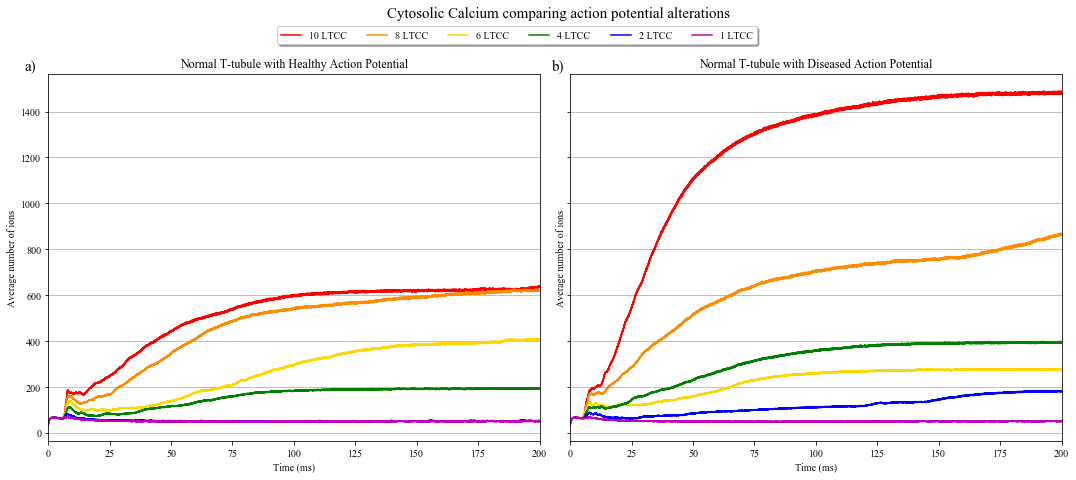
\includegraphics[scale=0.42]{cytCa_hnhd_Comparison.png}
	\caption{Cytosolic Calcium comparing action potential alterations}
	\subcaption{Cytosolic calcium in Normal T-Tubules with healthy action potential across range of L-Type Calcium Channels; \textbf{(b)} Cytosolic calcium in Normal T-Tubules with diseased action potential across range of L-Type Calcium Channels;}
	\label{fig:hnhd Calcium}
\end{figure}

\setcounter{figure}{11}
\begin{figure}
\centering
	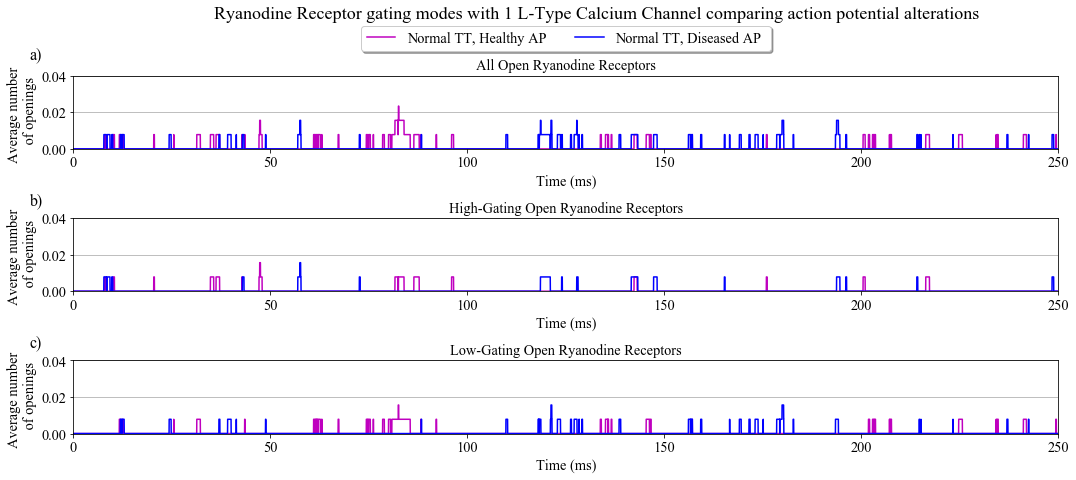
\includegraphics[scale=0.42]{hnhd1RyR_r_1AP_Comparison.png}
	\caption{Ryanodine Receptor gating modes with 1 L-Type Calcium Channel comparing action potential alterations}
	\subcaption{All open Ryanodine Receptors; \textbf{(b)} High-gating open Ryanodine Receptors; \textbf{(c)} Low-gating open Ryanodine Receptors: Healthy action potential (purple), Diseased action potential (blue)}
\label{fig:hnhd 1 LTCC 1 AP RyR} 
\end{figure}

\setcounter{figure}{12}
\begin{figure}
\centering
	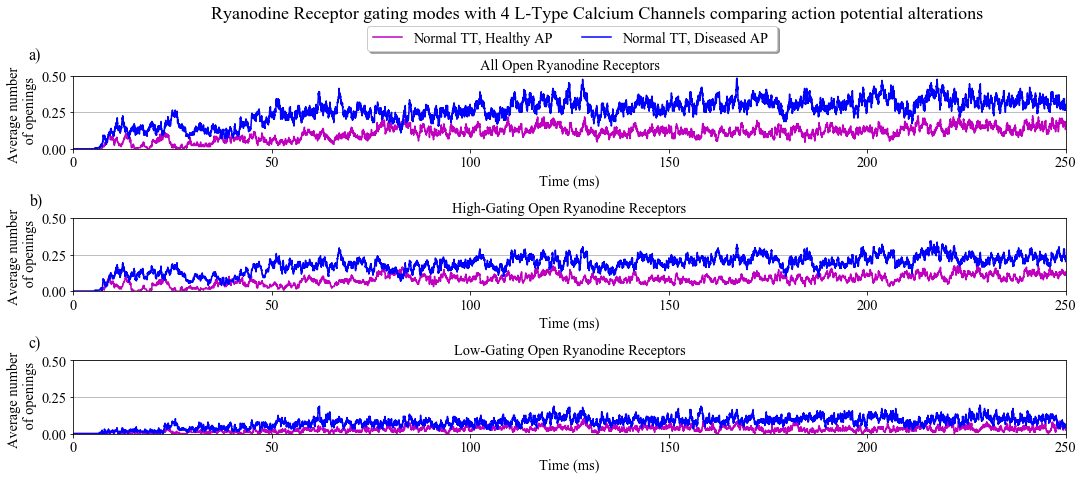
\includegraphics[scale=0.4]{hnhd4RyR_r_Comparison.png}
	\caption{Ryanodine Receptor gating modes with 4 L-Type Calcium Channels comparing action potential alterations}
	\subcaption{All open Ryanodine Receptors; \textbf{(b)} High-gating open Ryanodine Receptors; \textbf{(c)} Low-gating open Ryanodine Receptors; Healthy action potential (purple), Diseased action potential (blue)}
\label{fig:hnhd 4 LTCC 1 AP RyR} 
\end{figure}



\subsubsection{Geometric alterations}
In an additional effort to understand disease phenotypes in heart failure, we investigated the effects of T-Tubule deformations on cardiac calcium release units. In the literature, is effect is termed "de-tubulation" of myocyte tissue \cite{Louch2010}. Because of the close juxtaposition of T-Tubule membranes and SR membranes, we predicted an increase in the dyadic space would result in significantly less RyR activation and overall low rates SR calcium efflux, resulting in low cytosolic calcium. 

\setcounter{figure}{12}
\begin{figure}
\centering
	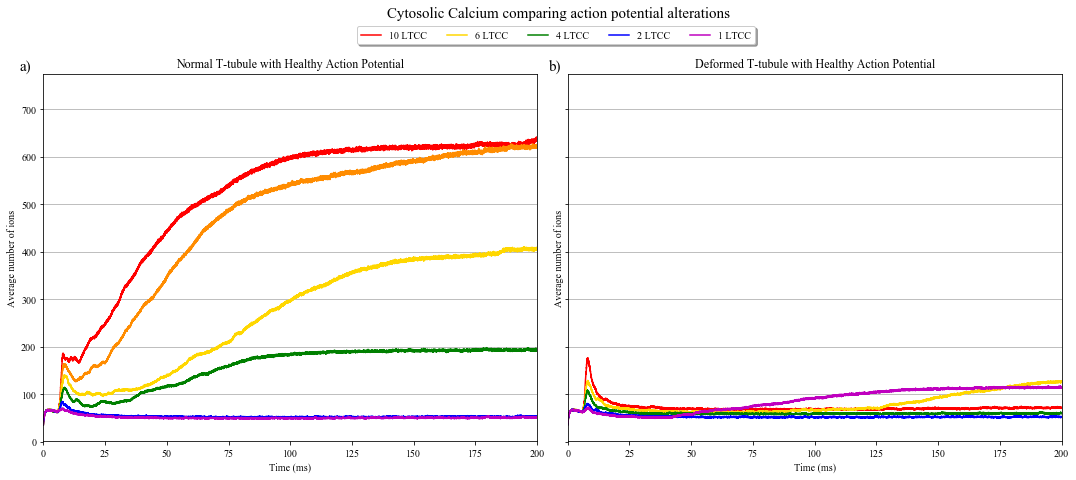
\includegraphics[scale=0.4]{cytCa_hndn_Comparison.png}
		\caption{Cytosolic Calcium Calcium dynamics comparing T-Tubule geometry alterations}
	\subcaption{Normal T-Tubule with Healthy action potential showing Calcium dynamics in the cytosol; \textbf{(b)} Deformed T-Tubule with Healthy action potential showing Calcium dynamics in the cytosol; 10 LTCC (red), 8 LTCC (orange), 6 LTCC (yellow), 4 LTCC (green), 2 LTCC (blue), 1 LTCC (purple)}
\label{fig:geometry comparison} 
\end{figure}


\setcounter{figure}{13}
\begin{figure}
\centering
	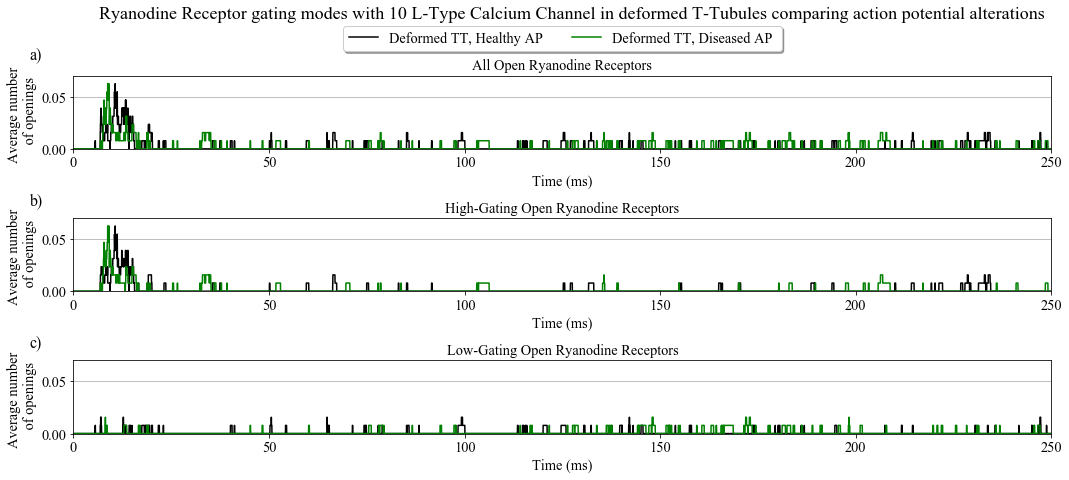
\includegraphics[scale=0.4]{dndd10RyR_r_Comparison.png}
	\caption{Ryanodine Receptor gating modes with 10 L-Type Calcium Channel in deformed T-Tubules comparing action potential alterations}
	\subcaption{All open Ryanodine Receptors; \textbf{(b)} High-gating open Ryanodine Receptors; \textbf{(c)} Low-gating open Ryanodine Receptors; Healthy action potential (black), Diseased action potential (green)}
\label{fig:hnhd 4 LTCC 1 AP RyR} 
\end{figure}

Our results validated our hypothesis, showing little to no calcium spark activity in deformed cells when compared to healthy cells (see figure 4.13). A similar distance (40 nm displacement of TT2) was used by Koh et al. \cite{Koh2006}, who reported similar results. In future simulations, we will successively increase the dyadic volume in order to further analyze the effect of disease progression, systematically. 


An interesting result of our simulations was the compensation effect exhibited by disease action potentials in simulations of diseased geometries. We compared the activation profiles of healthy and diseased action potentials in diseased geometries in our experiments. Under these conditions, the disease action potentials lead to more RyR flux events even in the diseased morphologies (see figure 14). Even with a dramatic detubulation, this effect is still visible.

We hypothesize that at less severe levels of T-Tubule deformations, the disease AP compensation effect will be pronounced enough to compensate for the deformity. Ideally, we will apply our MCell model to new tomographic CRU geometries from both healthy and diseased myocytes to gain more insights into the potential for compensation by affected action potentials.

\subsubsection{Modeling Ryanodine Receptor dispersion}
The use of a stochastic spatial technique combined Markov Model of RyR marks a significant advancement in the realistic modeling of calcium sparks, in stark contrast to phenomenological, deterministic, continuum models of RyR that are traditionally used to describe Ca\textsuperscript{2+} sparks \cite{Maleckar2017}. With the use of Markov Model descriptions of RyR, we are able to directly investigate the phenomenon of Calcium-Induced Calcium Release. The spatial representations exhibited in our model of the CRU importantly allow for investigation of the effects of disease phenotypes that implicate RyR.

\setcounter{figure}{14}
\begin{figure}
\centering
	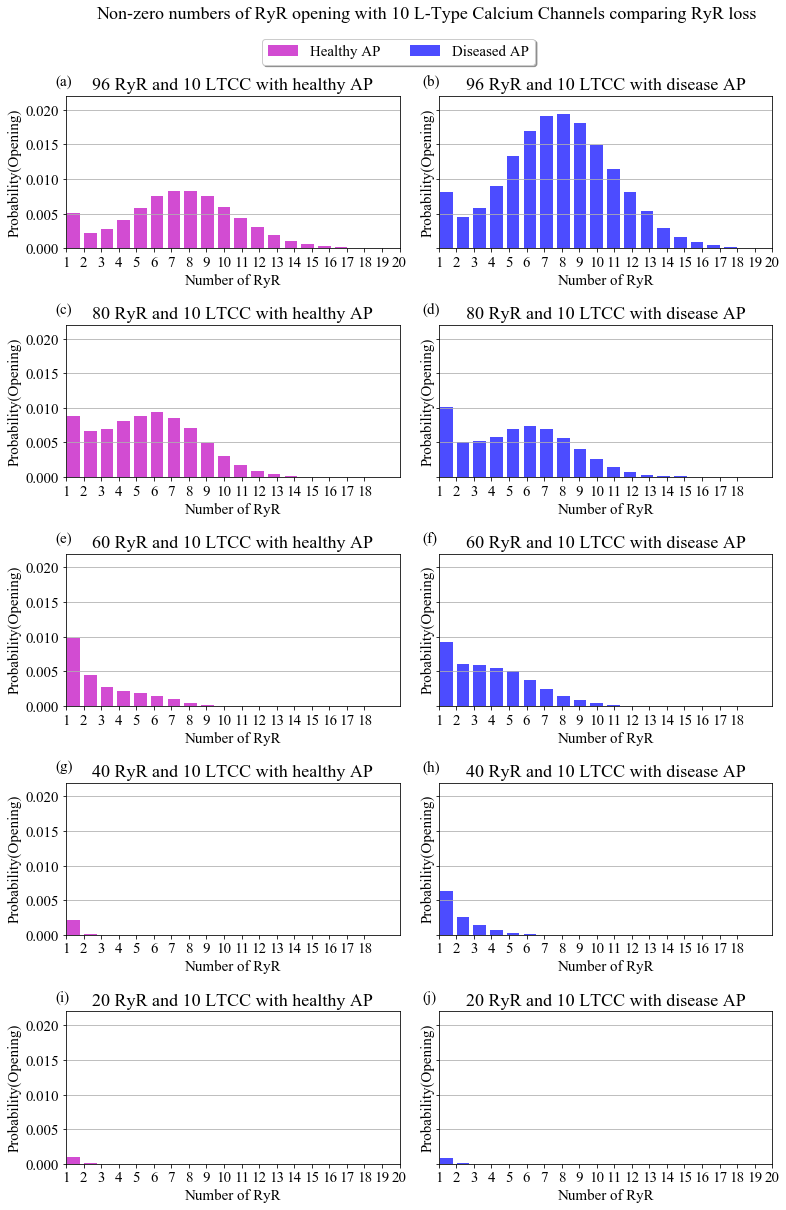
\includegraphics[scale=0.4]{orphanedRyR_hnhd_Comparison.png}
		\caption{Non-zero numbers of RyR opening with 10 L-Type Calcium Channels comparing RyR loss}
	\subcaption{Number of RyR open of 96 total with healthy AP; \textbf{(b)} Number of RyR open of 96 total with diseased AP; \textbf{(c)} Number of RyR open of 80 total with healthy AP; \textbf{(d)} Number of RyR open of 80 total with diseased AP; \textbf{(e)} Number of RyR open after 3 normal action potential stimuli in healthy t-tubules; \textbf{(f)}Number of RyR open after 3 diseased action potential stimuli in healthy t-tubules; \textbf{(g)} Number of RyR open after 4 normal action potential stimuli in healthy t-tubules; \textbf{(g)}Number of RyR open after 4 diseased action potential stimuli in healthy t-tubules; \textbf{(i)} Number of RyR open after 5 normal action potential stimuli in healthy t-tubules; \textbf{(j)}Number of RyR open after 5 diseased action potential stimuli in healthy t-tubules; Healthy action potential (pink), Diseased action potential (blue).}
\label{fig:probabilities} 
\end{figure}


It has been shown by multiple investigators that RyR function and localization are affected by heart failure \cite{Ather2013}. More specifically, regulators of RyR including PKA \cite{Vest2006} and CaMKII \cite{Hoch1999} have been implicated in altered calcium signaling. In heartfailure, RyR dispersion, or loss of RyR in junctional SR has been observed and shown to have pronounced effects on Ca\textsuperscript{2+} signaling \cite{Kolstad2018}. Earlier reports have determined that 50\% RyR loss results in significant alterations in firing propensity at the level that can be detected by cellular imaging and biochemical measurements \cite{Bround2016}. In order to visualize these effects on the molecular level, we performed simulations within our CRU  and successively removed clusters of RyR in the junctional space. Starting from a baseline of 96 RyR as imaged in the original CRU \cite{Hayashi2009}, we successively deleted clusters of RyR for a total of 80, 60, 40, 20, and 10 Ryanodine Receptors juxtaposed against 10 L-Type Calcium Channels, the results of which are shown in figure 15. 

As we decrease the number of RyR from 96 to 80 (figure 15 a-d) we see a dramatic decrease in the disease AP case. This is likely because of the phenomenon of CICR, where RyR efflux activates neighboring RyR. The decreae also affects the peak levels of RyR which in the former case are 7-10 RyR open at a time, and in the latter case 5-7. Decreasing the number of RyR to 60 (figure 15 e,f) significantly affects the number of RyR that can be activated as well as the total range of RyR that are open. As we decrease the number of RyR by more than half, to 40 (figure 15 g-i), it becomes nearly impossible to see activation of RyR. These results are consistent with previous reports that demonstrate a 50\% decrease in junctional SR RyR results in significant alterations in activation \cite{Bround2016}.


\subsection{Simulating "heartbeats" with successive action potentials}

The single action potential stimulation of Ryanodine receptors in the realistic geometry is a significant step towards realistic modeling of CICR. However, there are caveats to usage of single action potentials. Namely, these action potentials affect systems starting from equilibrium. In rapidly stimulated cells such as the mouse heart, which beats at a rate of 600 bpm, the system is hardly at equilibrium ever. The constant stimulation of these cells means that to accurately depict the complexity of the subcellular landscape, we must subject the cell to similar stimulation. 

\setcounter{figure}{16}
\begin{figure}
\centering
	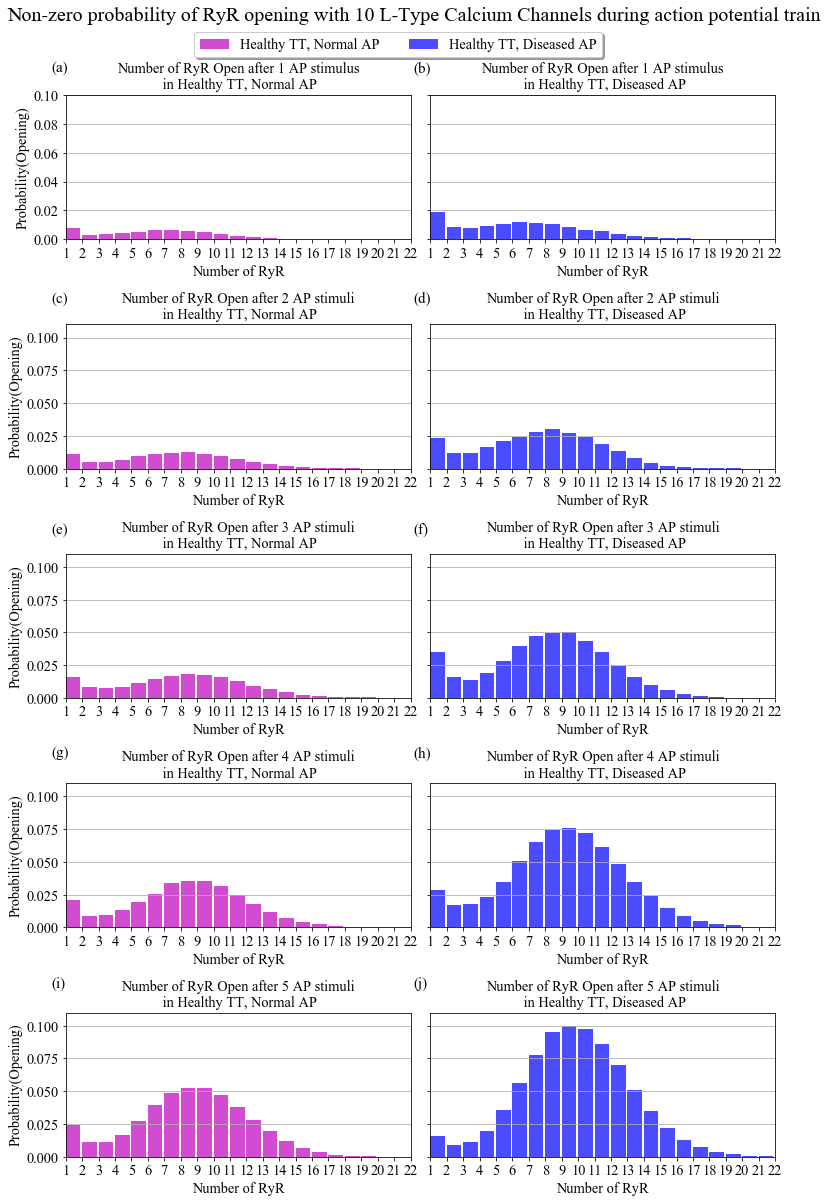
\includegraphics[scale=0.4]{probabilities_RyRopen_hnhd_1-5_AP_Comparison.png}
		\caption{Non-zero probability of RyR opening with 10 L-Type Calcium Channels during an action potential train}
	\subcaption{Number of RyR open after 1 normal action potential stimulus in healthy t-tubules; \textbf{(b)} Number of RyR open after 1 diseased action potential stimulus in healthy t-tubules; \textbf{(c)} Number of RyR open after 2 normal action potential stimuli in healthy t-tubules; \textbf{(d)} Number of RyR open after 2 diseased  action potential stimuli in healthy t-tubules; \textbf{(e)} Number of RyR open after 3 normal action potential stimuli in healthy t-tubules; \textbf{(f)}Number of RyR open after 3 diseased action potential stimuli in healthy t-tubules; \textbf{(g)} Number of RyR open after 4 normal action potential stimuli in healthy t-tubules; \textbf{(g)}Number of RyR open after 4 diseased action potential stimuli in healthy t-tubules; \textbf{(i)} Number of RyR open after 5 normal action potential stimuli in healthy t-tubules; \textbf{(j)}Number of RyR open after 5 diseased action potential stimuli in healthy t-tubules; Healthy action potential (pink), Diseased action potential (blue)}
\label{fig:probabilities} 
\end{figure}

In order to model this successive stimulation that underlies the heartbeat of a mouse, we performed simulations that feature successive LTCC impulses for both healthy and diseased cases AP cases. We then examined the open probability of RyR opening at successive APs, the results of which are shown in figure 16. Similarly to our earlier experiments, the disease action potential is, overall, more pronounced than the healthy action potential (figure 16 a-i). Between the first and the second action potential, the differences are slightly increased, meaning that the CRUs are more sensitized after a second AP. By the third AP, the differences between the healthy and diseased APs become more significant, with the peak number of RyR firing shifting towards the range of number of RyR open shifting from
a single RyR opening to a range of four to seven (figure 16 c,d). Additionally, the probability of firing increases significantly from under 0.01 after a single AP to about 0.02 as we move to the third AP (figure 16 e,f). By the third AP, the cell peaks at a range of seven to ten RyR open at a time of stimulation by a healthy AP. This peak number of open RyR is maintained as the action potentials increase (figure 16 g-i). Most interestingly, the diseased AP stimulated RyR are twice more likely to open in similar ranges of number of RyR activated (seven to ten). The successive action potentials (4AP and 5AP) only serve to sensitize the cell further. The ranges of RyR likely to fire after the 5th AP are at a maximal level in the diseased case. In future simulations, it will be important to gather our observations after the system has equilibrated, giving similar activation profiles after each AP. This will potentially require ten to fifteen successive APs because RyR are known to activate one-another in CICR, which at present, is computationally prohibitive (10 days/10 APs in a single system).


\subsection{Model caveats and future directions}
Though our model yields significant insights into subcellular Ca\textsuperscript{2+} dynamics in myocardial CRUs, it is not without its shortcomings. First, the CRU geometry offers an n=1, meaning a low sample size with regards to spatial geometry variation, specifically the SR. An advantage of using MCell is the ability to import new segmented meshes within which the dynamics can be computed. With the development of new technologies to image \cite{Kolstad2018} and reconstruct \cite{Lee2018} cellular ultrastructure, this limitation can be remedied through the application of the system dynamics to new geometries.

Secondly, our model samples the dynamics of a small slice of the myocyte which is bound by a cytosolic region of size 1.43$\times$9.40$\times$4.06$\mu$M. This geometry is not large enough to fully encapsulate the effects that neighboring CRUs have on activation by CICR. To capture these dynamics, it is necessary to modulate the boundary condition of our cytosolic compartment. We plan to test different boundary conditions, whether they be reflective or absorptive, or even the addition of more cytosolic compartments as was done Hake et al. \cite{Hake2012}. As of yet, our conversations with our continuum-modeling collaborators have not converged to what is "best-fit" for an explicit particle system like our own. 

Because our system tracks the individual motions of every molecule in the system explicitly as well as all molecular reactions, large compute resources are required for sampling. Our present simulations are results from a total of 128 simulations per system (Normal T-Tubule, Healthy AP, etc). The systems that sampled only a single action potential equal to 3,840 independent simulations/30 systems. Adding in the simulations of RyR permutations sets us at over 5,000 individial simulations. Gathering accurate statistics for events that are rare to sample, such as single AP activated CICR, requires larger sampling of the system (on the order of 10,000 simulations or more). The results we report here are preliminary and likely to be exhibited in larger population sampling cases. Nevertheless, we admit that additional sampling is required to gain insight about confidence intervals and errors. 

Molecular distribution is a key facet of spatial modeling methods.It is extremely likely that molecular distribution is non-linear. That is, molecular microdomains exist within the cytoplasmic region. At present, our model has not investigated the potential for protein localization alterations to influence our results. In future simulations, these effects can be directly interrogated using the special modeling techniques that we employ. The totality of the complex biochemical underpinnings of CICR are only partially explored by this model. Additional complexity is added when considering the regulation of the proteins on membranous surfaces like SERCA and RyR and of proteins in the cytosol like actin and myosin. To move towards a holistic and realistic understanding of CICR, it is necessary to include these species as they are known to play a vital role in cell function and disease states \cite{Ather2013}. 

Our system required very little parameterization in order to produce the results that have been discussed. A study addressing the sensitivity of parameters in our system is required To determine which variables are most likely to influence simulation results.For the purpose of peer review, it will be necessary to produce such reports. 

Finally, to understand the effects of molecular crowding in systems with low molecular concentrations, it is not sufficient to represent molecular species as point particles.To address this, we have formed a collaboration with investigators at the Scripps Research Institute who have developed molecular packing algorithms that yield an accurate, atomic-level description Of our system. The program we used for molecular packing is called cellPACK \cite{Johnson2014}, And has been used in the past to visualize molecular dynamics simulations of an entire virus (unpublished). This cutting-edge visualization and packing technology can be combined with the reaction-diffusion powers of MCell to visualize the subcellular dynamics of our system at the finest level of molecular detail. 

\section{Conclusion}
This chapter has laid out the details used to build the first-ever spatial, discrete model of subcellular calcium signaling mechanisms in realistic geometries of left ventricle mouse myocardium. The power of this model is not to be understated, as it can easily translate and be applied to any segmented and meshed geometry obtained from electron microscopy methods. Arguably the most important facet of the model is the ability to count low numbers of calcium ions in parts of our geometry. Our simulations confirm the suspicions of those who intuit cardiomyocyte mechanics. Namely, that the average number of Ca\textsuperscript{2+} ions in the junctional dyadic cleft \textit{are} zero at equilibrium \cite{Bers2002}.

Our model features a stochastic representation of Ryanodine Receptor dynamics that responds to local increases of cytosolic calcium. Coupling this advancement with the introduction of a voltage activated L-Type Calcium Channel model makes our model a suitable candidate for more-accurate description of the molecular-level details underlying cardiac calcium activation mechanisms. We incorporate discrete adaptations to existing SERCA model dynamics that satisfy microscopic reversibility \cite{Higgins2006}. Building upon the sophistication of the original CRU model by Hake et al. \cite{Hake2012}, we have moved towards towards a more realistic representation of the subcellular biochemistry. 

Our investigations have determined that disease phenotypes are detectable on the level of single molecules in subcellular geometries. Our interrogation of disease action potentials resemble late calcium sparks that have been reported in the literature \cite{Fowler2017}. Using realistic geometries \cite{Hayashi2009}, we explored the effects of deformation on the junctional T-Tubule and demonstrated that drastic detubulation severely affects subcellular calcium handling, consistent with the observations of others \cite{Crossman2015,Louch2010}. Finally, we suggest that disease APs have a compensatory effect for deformations on the subcellular level.

\section{Acknowledgments}

Chapter 4 is currently being prepared for submission for
publication of the material. \textbf{\underline{Hirakis, Sophia P.}};  Bartol, Thomas M.; Sejnowski, Terrence, J; Amaro, Rommie E; The dissertation author was the primary investigator and author of this material.

This work would not have been possible without the scientific collaboration, expertise and aide of the following people, whom we wish to formally acknowledge. First, we thank Dr. Johan E. Hake for his help in translating his original model in our study. We thank Dr. Andrew G. Edwards for his constant mentorship and advice in designing the simulations of the system. Dr. Andrew D. McCulloch also aided in the system design and contextualization of observations. We thank Dr. Eric E. Sobie for his frequent discussions on model scope and design. We acknowledge the lab of Dr. David D. Thomas, and especially Dr. J. Michael Autry for his frequent discussions on SERCA function. We acknowledge Dr. J. Andrew McCammon for his support of the project, and Dr. Rommie E. Amaro for pushing the model to completion. We acknowledge Dr. Terrence J. Sejnowski for his support and the entire lab for their feedback, especially Jorge Aldana for his support in computing resources. We thank Robert Kuczewski for his constant support and development of MCell.  I would like to explicitly acknowledge Dr. Thomas M. Bartol for working tirelessly to develop this model with me for the greater half of the last decade; I would be nowhere without you. 

 \section{Supplementary Information}
 
\begin{table}[h]
\centering
\caption{Parameters of Calcium buffering species}
\resizebox{\textwidth}{!}{\begin{tabular}{ccccc}
\hline
\textbf{Parameter} & \textbf{Description} & \textbf{Value} & 
\textbf{Units} & \textbf{Reference} \\
\hline
D$^{cyt}$$_{Ca}$ & Diffusion constant of Ca$^{2+}$ (in cytosol 
and SR) & 2.2 x 10$^{6}$ & cm$^{2}$s$^{-1}$ & Hake et al. 
(2012); Louch et al. (2010) \\
\hline
D$^{cyt}$$_{ATP\_Ca}$ & Diffusion constant of Ca$^{2+}$-bound 
ATP in cytosol & 1.4 x 10$^{-6}$ & cm$^{2}$s$^{-1}$ & Hake et 
al. (2012); Valent et al (2007) \\
\hline
$[$Ca$^{2+}$$]$$_{cyt}$ & Initial Concentration of Ca$^{2+}$ 
in cytosol & 140 x 10$^{-9}$ & M & Hake et al. (2012) \\
\hline
$[$ATP$]$$_{cyt}$ & Free ATP concentration in cytosol & 454.682 x 10
$^{-6}$ & M & Hake et al. (2012); Bers (2001) \\
\hline
$[$ATP-Ca$]$$_{cyt}$ & Ca$^{2+}$-bound ATP concentration in 
cytosol & 318 x 10$^{-9}$ & M & Hake et al. (2012) \\
\hline
$^{ATP}$k$_{on}$ & ATP Ca$^{2+}$ on rate constant & 2.25 x 10$^{8}$ & 
M$^{-1}$s$^{-1}$ & Hake et al. (2012); Picht et al. (2011); Bers 
(2001) \\
\hline
$^{ATP}$k$_{off}$ & ATP Ca$^{2+}$ off rate constant & 450 x 10$^{2}$ 
& s$^{-1}$ & Hake et al. (2012); Picht et al. (2011) \\
\hline
D$^{cyt}$$_{CMDN}$ & Diffusion constant of Calmodulin in cytosol & 
25 x 10$^{-8}$ & cm$^{2}$s$^{-1}$ & Hake et al. (2012); 
Michailova et al. (2002) \\
\hline
D$^{cyt}$$_{CMDN\_Ca}$ & Diffusion constant of Ca$^{2+}$-bound 
Calmodulin in cytosol & x 10$^{-6}$ & cm$^{2}$s$^{-1}$ & Hake 
et al. (2012); \\
\hline
$[$CMDN$]$$_{cyt}$ & Free Calmodulin concentration in cytosol & 
23.529 x 10$^{-6}$ & M & Hake et al. (2012); Fabiato (1983) \\
\hline
$[$CMDN-Ca$]$$_{cyt}$ & Ca$^{2+}$-bound Calmodulin concentration 
in cytosol & 471 x 10$^{-9}$ & M & Hake et al. (2012) \\
\hline
$^{CMDN}$k$_{on}$ & Calmodulin Ca$^{2+}$ on rate constant & 34 x 10$^{
6}$ & M$^{-1}$s$^{-1}$ & Hake et al. (2012); Robertson et al 
(1981); Picht et al. (2011) \\
\hline
$^{CMDN}$k$_{off}$ & Calmodulin Ca$^{2+}$ off rate constant & 238 & s
$^{-1}$ & Hake et al. (2012); Robertson et al (1981) \\
\hline
D$^{cyt}$$_{TRPN}$ & Diffusion constant of Troponin-C in cytosol & 
0 & cm$^{2}$s$^{-1}$ & Hake et al. (2012) \\
\hline
D$^{cyt}$$_{TRPN\_Ca}$ & Diffusion constant of Ca$^{2+}$-bound 
Troponin-C in cytosol & 0 & cm$^{2}$s$^{-1}$ & Hake et al. (2012) 
\\
\hline
$[$TRPN$]$$_{cyt}$ & Free Troponin-C concentration in cytosol & 56.8 
x 10$^{-6}$ & M & Hake et al. (2012); Bondarenko et al. (2004) \\
\hline
$[$TRPN-Ca$]$$_{cyt}$ & Ca$^{2+}$-bound Troponin-C concentration 
in cytosol & 13.2 x 10$^{-6}$ & M & Hake et al. (2012) \\
\hline
$^{TRPN}$k$_{on}$ & Troponin-C Ca$^{2+}$ on rate constant & 32.7 x 10
$^{6}$ & M$^{-1}$s$^{-1}$ & Hake et al. (2012); Bondarenko et 
al. (2004) \\
\hline
$^{TRPN}$k$_{off}$ & Troponin-C Ca$^{2+}$ off rate constant & 19.6 & s
$^{-1}$ & Hake et al. (2012); Bondarenko et al. (2004) \\
\hline
D$^{cyt}$$_{Fluo4}$ & Diffusion constant of Fluo-4 in cytosol & 42 
x 10$^{-8}$ & cm$^{2}$s$^{-1}$ & Hake et al. (2012); Picht et 
al. (2011) \\
\hline
D$^{cyt}$$_{Fluo4\_Ca}$ & Diffusion constant of Ca$^{2+}$
-bound Fluo-4 in cytosol & 42 x 10$^{-8}$ & cm$^{2}$s$^{-1}$ & 
Hake et al. (2012) \\
\hline
$[$Fluo4$]$$_{cyt}$ & Free Fluo-4 concentration in cytosol & 22.186 x 
10$^{-6}$ & M & Hake et al. (2012); Picht et al. (2011) \\
\hline
$[$Fluo4-Ca$]$$_{cyt}$ & Ca$^{2+}$-bound Fluo-4 concentration in 
cytosol & 2.82 x 10$^{-6}$ & M & Hake et al. (2012) \\
\hline
$^{Fluo4}$k$_{on}$ & Fluo-4 Ca$^{2+}$ on rate constant & 110 x 10$^{6
}$ & M$^{-1}$s$^{-1}$ & Hake et al. (2012); Picht et al. (2011) 
\\
\hline
$^{Fluo4}$k$_{off}$ & Fluo-4 Ca$^{2+}$ off rate constant & 110 & s$^{
-1}$ & Hake et al. (2012); Picht et al. (2011) \\
\hline
D$^{cyt}$$_{Fluo5}$ & Diffusion constant of Fluo-5 in cytosol & 8 
x 10$^{-8}$ & cm$^{2}$s$^{-1}$ & Hake et al. (2012); Picht et 
al. (2011) \\
\hline
D$^{cyt}$$_{Fluo5\_Ca}$ & Diffusion constant of Ca$^{2+}$
-bound Fluo-5 in cytosol & 8 x 10$^{-8}$ & cm$^{2}$s$^{-1}$ & 
Hake et al. (2012) \\
\hline
$[$Fluo5$]$$_{cyt}$ & Free Fluo-5 concentration in cytosol & 5.9 x 10
$^{-6}$ & M & Hake et al. (2012); Picht et al. (2011) \\
\hline
$[$Fluo5-Ca$]$$_{cyt}$ & Ca$^{2+}$-bound Fluo-5 concentration in 
cytosol & 19.1 x 10$^{-6}$ & M & Hake et al. (2012) \\
\hline
$^{Fluo5}$k$_{on}$ & Fluo-5 Ca$^{2+}$ on rate constant & 110 x 10$^{6
}$ & M$^{-1}$s$^{-1}$ & Hake et al. (2012); Picht et al. (2011) 
\\
\hline
$^{Fluo5}$k$_{off}$ & Fluo-5 Ca$^{2+}$ off rate constant & 110 & s$^{
-1}$ & Hake et al. (2012) \\
\hline
D$^{sr}$$_{CSQN}$ & Diffusion constant of Calsequestrin in cytosol 
& 0 & cm$^{2}$s$^{-1}$ & Hake et al. (2012) \\
\hline
D$^{sr}$$_{CSQN\_Ca}$ & Diffusion constant of Ca$^{2+}$-bound 
Calsequestrin in SR & 0 & cm$^{2}$s$^{-1}$ & Hake et al. (2012) 
\\
\hline
$[$CSQN$]$$_{cyt}$ & Free Calsequestrin concentration in SR & 56.8 x 
10$^{-6}$ & M & Hake et al. (2012); Bondarenko et al. (2004) \\
\hline
$[$CSQN-Ca$]$$_{cyt}$ & Ca$^{2+}$-bound Calsequestrin 
concentration in SR & 13.2 x 10$^{-6}$ & M & Hake et al. (2012) \\
\hline
$^{CSQN}$k$_{on}$ & Calsequestrin Ca$^{2+}$ on rate constant & 32.7 x 10
$^{6}$ & M$^{-1}$s$^{-1}$ & Hake et al. (2012); Bondarenko et 
al. (2004) \\
\hline
$^{CSQN}$k$_{off}$ & Calsequestrin Ca$^{2+}$ off rate constant & 19.6 & 
s$^{-1}$ & Hake et al. (2012); Bondarenko et al. (2004) \\
\hline
\end{tabular}}
\end{table}


\begin{table}[h]
\centering
\caption{Parameters for Sodium-Calcium Exchanger (NCX) 
and Plasma Membrane Calcium-ATPase (PMCA) pump models}
\resizebox{\textwidth}{!}{\begin{tabular}{cccc}
\hline
\textbf{Parameter} & \textbf{Value} & \textbf{Units} & \textbf{
Reference} \\
\hline
k$_{P0P1}$ & 1.5 x 10$^{8}$ & M$^{-1}$s$^{-1}$ & Bartol et 
al. (2015); Brini and Carafoli (2009); Penheiter et al. (2003) \\
\hline
k$_{P0P1}$ & 15 & s$^{-1}$ & Bartol et al. (2015); Brini and 
Carafoli (2009); Penheiter et al. (2003) \\
\hline
k$_{P0P1\_pump}$ & 12 & s$^{-1}$ & Bartol et al. (2015); Brini and 
Carafoli (2009); Penheiter et al. (2003) \\
\hline
k$_{PMCA\_leak}$ & 5.25 & s$^{-1}$ & Yields 140nM Cytosolic 
Calcium \\
\hline
k$_{N0N1}$ & 3.0 x 10$^{8}$ & M$^{-1}$s$^{-1}$ & Bartol et 
al. (2015); Hilgemann(1991) \\
\hline
k$_{N1N0}$ & 300 & s$^{-1}$ & Bartol et al. (2015); Hilgemann(1991) 
\\
\hline
k$_{N1N0\_pump}$ & 600 & s$^{-1}$ & Bartol et al. (2015); 
Hilgemann(1991) \\
\hline
k$_{NCX\_leak}$ & 26.75 & s$^{-1}$ & Yields 140nM Cytosolic 
Calcium \\
\hline
\end{tabular}}
\end{table}


\begin{table}[h]
\centering
\caption{Parameters for L-Type Calcium Channel model}
\begin{tabular}{cccc}
\hline
\textbf{Parameter} & \textbf{Value} & \textbf{Units} & \textbf{
Reference} \\
\hline
a & 2 & - & Greenstein and Winslow (2002) \\
\hline
b & 1.9356 & - & Greenstein and Winslow (2002) \\
\hline
f & 850 & s$^{-1}$ & Greenstein and Winslow (2002) \\
\hline
g & 2000 & s$^{-1}$ & Greenstein and Winslow (2002) \\
\hline
f' & 5 & s$^{-1}$ & Greenstein and Winslow (2002) \\
\hline
g' & 7000 & s$^{-1}$ & Greenstein and Winslow (2002) \\
\hline
$\gamma$ & 0.44 x 10$^{6}$ & M$^{-1}$s$^{-1}$ & Greenstein and 
Winslow (2002) \\
\hline
$\omega$ & 0.02158 x 10$^{3}$ & s$^{-1}$ & Greenstein and Winslow (2002) 
\\
\hline
T & 310 & K & - \\
\hline
F & 96.485 x 10$^{3}$ & C/mol & - \\
\hline
N$_{A}$ & 6.02214 x 10$^{23}$ & \#/mol & - \\
\hline
P$_{Ca}$ & 9.13 x 10$^{-16}$ & L/s & - \\
\hline
\end{tabular}
\end{table}

\begin{table}[h]
\centering
\caption{Parameters for Ryanodine Receptor Markov model}
\begin{tabular}{cccc}
\hline
\textbf{Parameter} & \textbf{Value} & \textbf{Units} & \textbf{
Reference} \\
\hline
k$_{C1C2\_H1}$ & 3.26 x 10$^{6}$ & M$^{-1}$s$^{-1}$ & 
Saftenku et al. (2001) \\
\hline
k$_{C2C1\_H1}$ & 116 & s$^{-1}$ & Saftenku et al. (2001) \\
\hline
k$_{C2C3\_H1}$ & 0.66 x 10$^{6}$ & M$^{-1}$s$^{-1}$ & 
Saftenku et al. (2001) \\
\hline
k$_{C3C2\_H1}$ & 163 & s$^{-1}$ & Saftenku et al. (2001) \\
\hline
k$_{C1C2\_L}$ & 1.24 x 10$^{6}$ & M$^{-1}$s$^{-1}$ & 
Saftenku et al. (2001) \\
\hline
k$_{C2C1\_L}$ & 13.6 & s$^{-1}$ & Saftenku et al. (2001) \\
\hline
k$_{C2C3\_L}$ & 29.8 x 10$^{6}$ & M$^{-1}$s$^{-1}$ & 
Saftenku et al. (2001) \\
\hline
k$_{C3C2\_L}$ & 3867 & s$^{-1}$ & Saftenku et al. (2001) \\
\hline
k$_{C2C5\_L}$ & 1.81 & s$^{-1}$ & Saftenku et al. (2001) \\
\hline
k$_{C5C2\_L}$ & 3.63 & s$^{-1}$ & Saftenku et al. (2001) \\
\hline
k$_{C1C2\_LH1}$ & 6.67 x 10$^{2}$ & M$^{-1}$s$^{-1}$ & 
Saftenku et al. (2001) \\
\hline
k$_{C2C1\_H1L}$ & 0.0833 & s$^{-1}$ & Saftenku et al. (2001) \\
\hline
k$_{C2C3\_LH1}$ & 6.67 x 10$^{2}$ & M$^{-1}$s$^{-1}$ & 
Saftenku et al. (2001) \\
\hline
k$_{C3C2\_H1L}$ & 0.0833 & s$^{-1}$ & Saftenku et al. (2001) \\
\hline
k$_{C3C4\_LH1}$ & 6.67 x 10$^{2}$ & M$^{-1}$s$^{-1}$ & 
Saftenku et al. (2001) \\
\hline
k$_{C4C3\_H1L}$ & 0.0833 & s$^{-1}$ & Saftenku et al. (2001) \\
\hline
k$_{C2O1\_H1}$ & 7.86 x 10$^{6}$ & M$^{-1}$s$^{-1}$ & 
Saftenku et al. (2001) \\
\hline
k$_{O1C2\_H1}$ & 1480 & s$^{-1}$ & Saftenku et al. (2001) \\
\hline
k$_{C3O2\_H1}$ & 7.77 x 10$^{6}$ & M$^{-1}$s$^{-1}$ & 
Saftenku et al. (2001) \\
\hline
k$_{O2C3\_H1}$ & 330 & s$^{-1}$ & Saftenku et al. (2001) \\
\hline
k$_{C3O1\_L}$ & 731.2 & s$^{-1}$ & Saftenku et al. (2001) \\
\hline
k$_{O1C3\_L}$ & 4185 & s$^{-1}$ & Saftenku et al. (2001) \\
\hline
k$_{C3O2\_L}$ & 24.5 & s$^{-1}$ & Saftenku et al. (2001) \\
\hline
k$_{O2C3\_L}$ & 156.5 & s$^{-1}$ & Saftenku et al. (2001) \\
\hline
k$_{C3O3\_L}$ & 8.5 & s$^{-1}$ & Saftenku et al. (2001) \\
\hline
k$_{O3C3\_L}$ & 111.7 & s$^{-1}$ & Saftenku et al. (2001) \\
\hline
k$_{C4O2\_L}$ & 415.3 & s$^{-1}$ & Saftenku et al. (2001) \\
\hline
k$_{O2C4\_L}$ & 1995 & s$^{-1}$ & Saftenku et al. (2001) \\
\hline
k$_{C4O3\_L}$ & 43.3 & s$^{-1}$ & Saftenku et al. (2001) \\
\hline
k$_{O3C4\_L}$ & 253.3 & s$^{-1}$ & Saftenku et al. (2001) \\
\hline
k$_{C4O2\_H1}$ & 2390 & s$^{-1}$ & Saftenku et al. (2001) \\
\hline
k$_{O2C4\_H1}$ & 298 & s$^{-1}$ & Saftenku et al. (2001) \\
\hline
k$_{RyR\_flux}$ & 1.09 x 10$^{9}$ & M$^{-1}$s$^{-1}$ & Guo 
et al. (2012) \\
\hline
\end{tabular}
\end{table}


\begin{table}[h]
\centering
\caption{Parameters for Sarco/Endoplasmic Reticulum 
Calcium-ATPase (SERCA) pump}
\begin{tabular}{cccc}
\hline
\textbf{Parameter} & \textbf{Value} & \textbf{Units} & \textbf{
Reference} \\
\hline
k$_{X0X1}$ & 2 x 10$^{8}$ & M$^{-1}$s$^{-1}$ & Bartol et 
al. (2015); Higgins et al. (2006) \\
\hline
k$_{X1X0}$ & 146.775 & s$^{-1}$ & Bartol et al. (2015); Higgins 
et al (2006\\
\hline
k$_{X1X2}$ & 1 x 10$^{8}$ & M$^{-1}$s$^{-1}$ & Bartol et 
al. (2015); Higgins et al. (2006) \\
\hline
k$_{X2X1}$ & 293.551 & s$^{-1}$ & Bartol et al. (2015); Higgins 
et al. (2006) \\
\hline
k$_{X2Y2}$ & 0.6 & s$^{-1}$ & Bartol et al. (2015); Higgins et al. 
(2006) \\
\hline
k$_{Y2X2}$ & 0.097 & s$^{-1}$ & Bartol et al. (2015); Higgins et 
al. (2006) \\
\hline
k$_{Y2Y1}$ & 60.03 & s$^{-1}$ & Bartol et al. (2015); Higgins et 
al. (2006) \\
\hline
k$_{Y1Y2}$ & 1 x 10$^{5}$ & M$^{-1}$s$^{-1}$ & Bartol et 
al. (2015); Higgins et al. (2006) \\
\hline
k$_{Y1Y0}$ & 30.015 & s$^{-1}$ & Bartol et al. (2015); Higgins et 
al. (2006) \\
\hline
k$_{Y0Y1}$ & 2 x 10$^{5}$ & M$^{-1}$s$^{-1}$ & Bartol et 
al. (2015); Higgins et al. (2006) \\
\hline
k$_{Y0X0}$ & 0.4 & s$^{-1}$ & Bartol et al. (2015); Higgins et al. 
(2006) \\
\hline
k$_{X0Y0}$ & 0.0012 & s$^{-1}$ & Bartol et al. (2015); Higgins et 
al. (2006) \\
\hline
\end{tabular}
\end{table}










\begin{comment}
\begin{quote}
All quotes of more than six lines, even though this one is not, are to
be indented 0.5'' from the left and 0.5'' from the right. These longer
quotes are to be single spaced. Don't forget to adjust for proper
spacing after the last line of the quoted material.
\end{quote}
The rest of the paragraph would continue as so.
\end{comment}

\begin{comment}
% Skipping a bunch of chapters
\setcounter{chapter}{50}
\chapter{Another chapter}
\setcounter{figure}{73}
\setcounter{table}{88}
\begin{figure}
\centering
\fbox{\hbox to.8\linewidth{\hss Another figure\hss}}
\caption{Another figure caption}
\end{figure}
\begin{table}
\centering
\caption{Another table caption}
\begin{tabular}{ccc}
\toprule
X&Y&Z\\
\midrule
a&b&c\\
\bottomrule
\end{tabular}
\end{table}
\begin{figure}
\caption{ASDF fig}
\end{figure}
\begin{table}
\caption{ASDF tab}
\end{table}
\end{comment}

\begin{comment}


Katja received PhD in 1967 at Cornell University with 
topic 
Effect of impurities on lattice vibrations in solids

Post-doc Rochester with 
Xerox corp (lab near academic kind) offered job to her and husband at the time. Only one could work in basic research

Statistic mechanitian moved from Maryland, Dr. Elliot Montroll 

Invited her for post-doc
"better expenditure than air conditioning"

Schuler and Walter Kohn 

Tenured at UC San Diego in 1973 in Chemistry department. Assigned to teach Physical chemistry to 200+ people. Didn't know what physical chemistry was. 

Stanley miller (worked with Harold Urey) let her borrow notes. 

The only woman in the department. 

First and only 50 years first woman chair of physics, chemistry, mathematics, and biology. 

Susan Taylor was one of the first women hired in the department. 




Margaret Burbidge- astrophysicist astronomer royal iisaac newton 
Joe Mayer


Perrin 
Old boy network hire
1963 hired aat UCSD 

January 1964 only graduate students and post docs 

PhD Harvard 
Frank Westheimer physical organic chemist interested in biomolecules
Physical organic molecules to biochemistry 
Isotope effects


10 month Post doc Berkley

Urey hall first buildings

Most famous for
as an educator

Most cited 2D NMR applied to chemical kinetics
Magnetic Circular Dichroism

On the PhD committee of grad student of George Faher
behavior of UV vis absorptions in a magnetic field

shooting photons right circular polarization positive angular momentum 
create excited states of angular momentum



wive vibronic borrowing of porphoryins 

exciting electronic and vibrational excitation
net angular momentum is combination of ekectronic and vibrational

negative angular momentum electronic
vibrational is positive net is positive 

J Chem Phys
negative a terms in magnetic circular dichroism 



100mV / 50 nm of membrane

Volt / meter
0.1 V / 50e-9
2 million volts/meter electric field

electric field volts per distance 

\begin{figure}
\centering

\begin{subfigure}[t]{.4\textwidth}
\centering
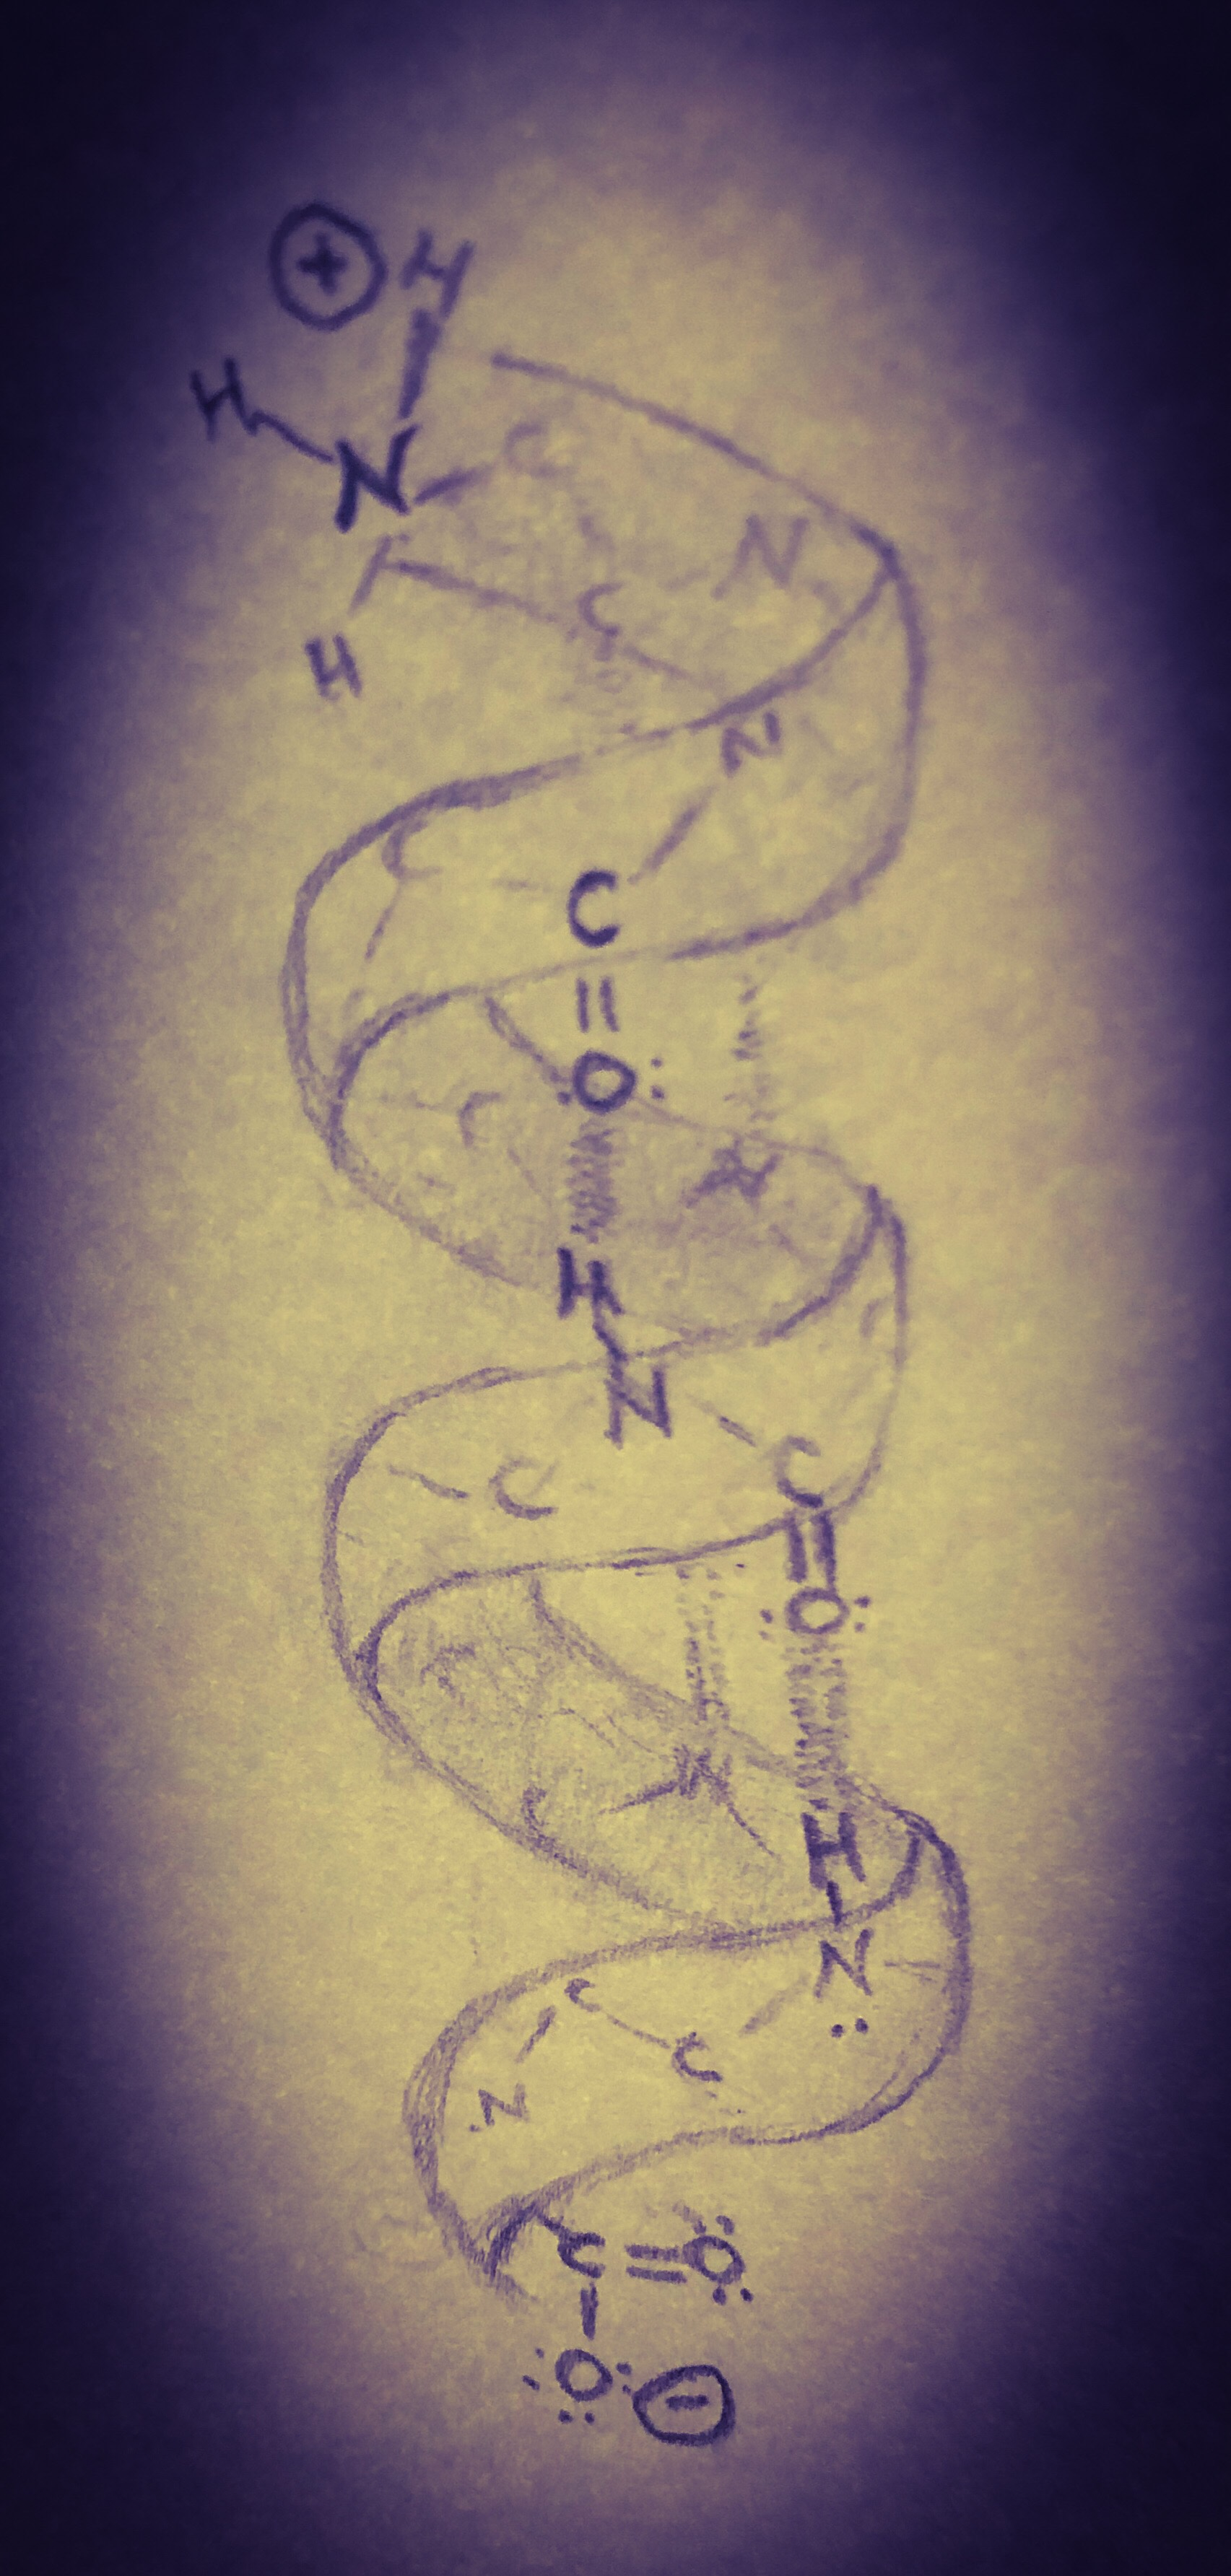
\includegraphics[width=0.6\linewidth]{helix.jpg}
        \caption{}\label{fig:fig_a}
\end{subfigure}
%
\begin{subfigure}[t]{.4\textwidth}
\centering
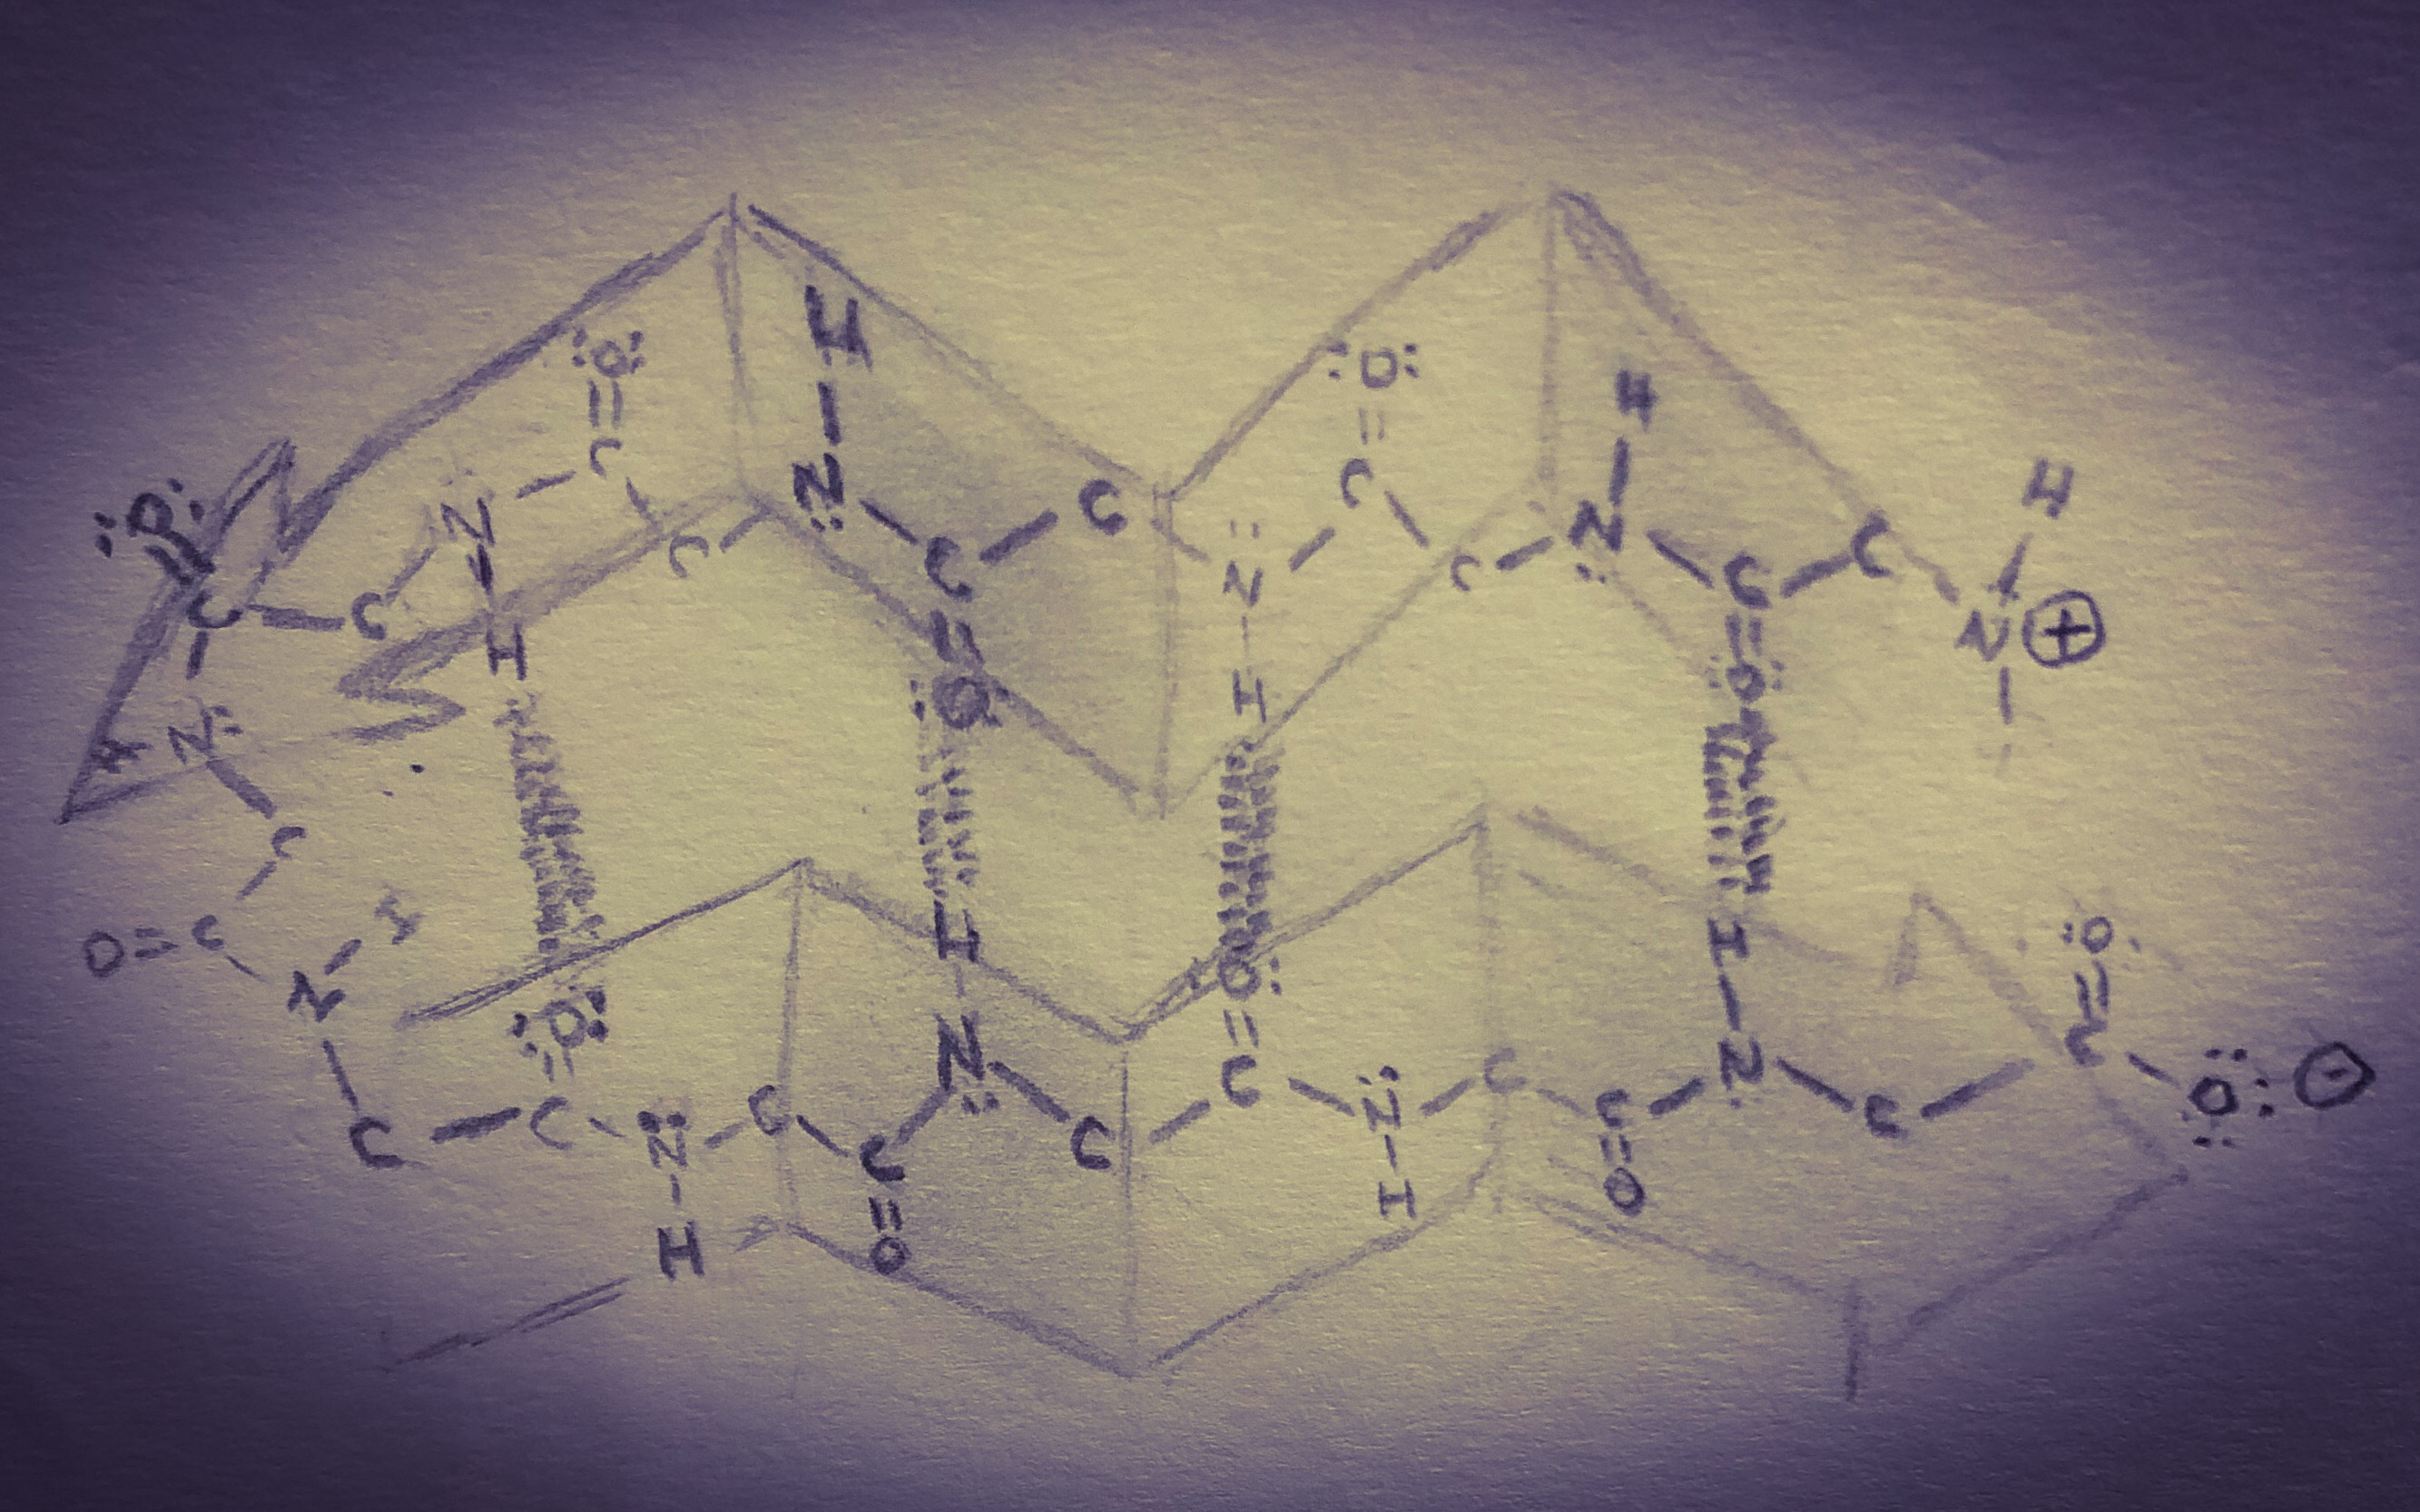
\includegraphics[width=1.3\linewidth]{sheet.jpg}
\caption{}\label{fig:fig_b}
\end{subfigure}



\begin{subfigure}[t]{.4\textwidth}
\centering
\vspace{0pt}% set the real top as the top
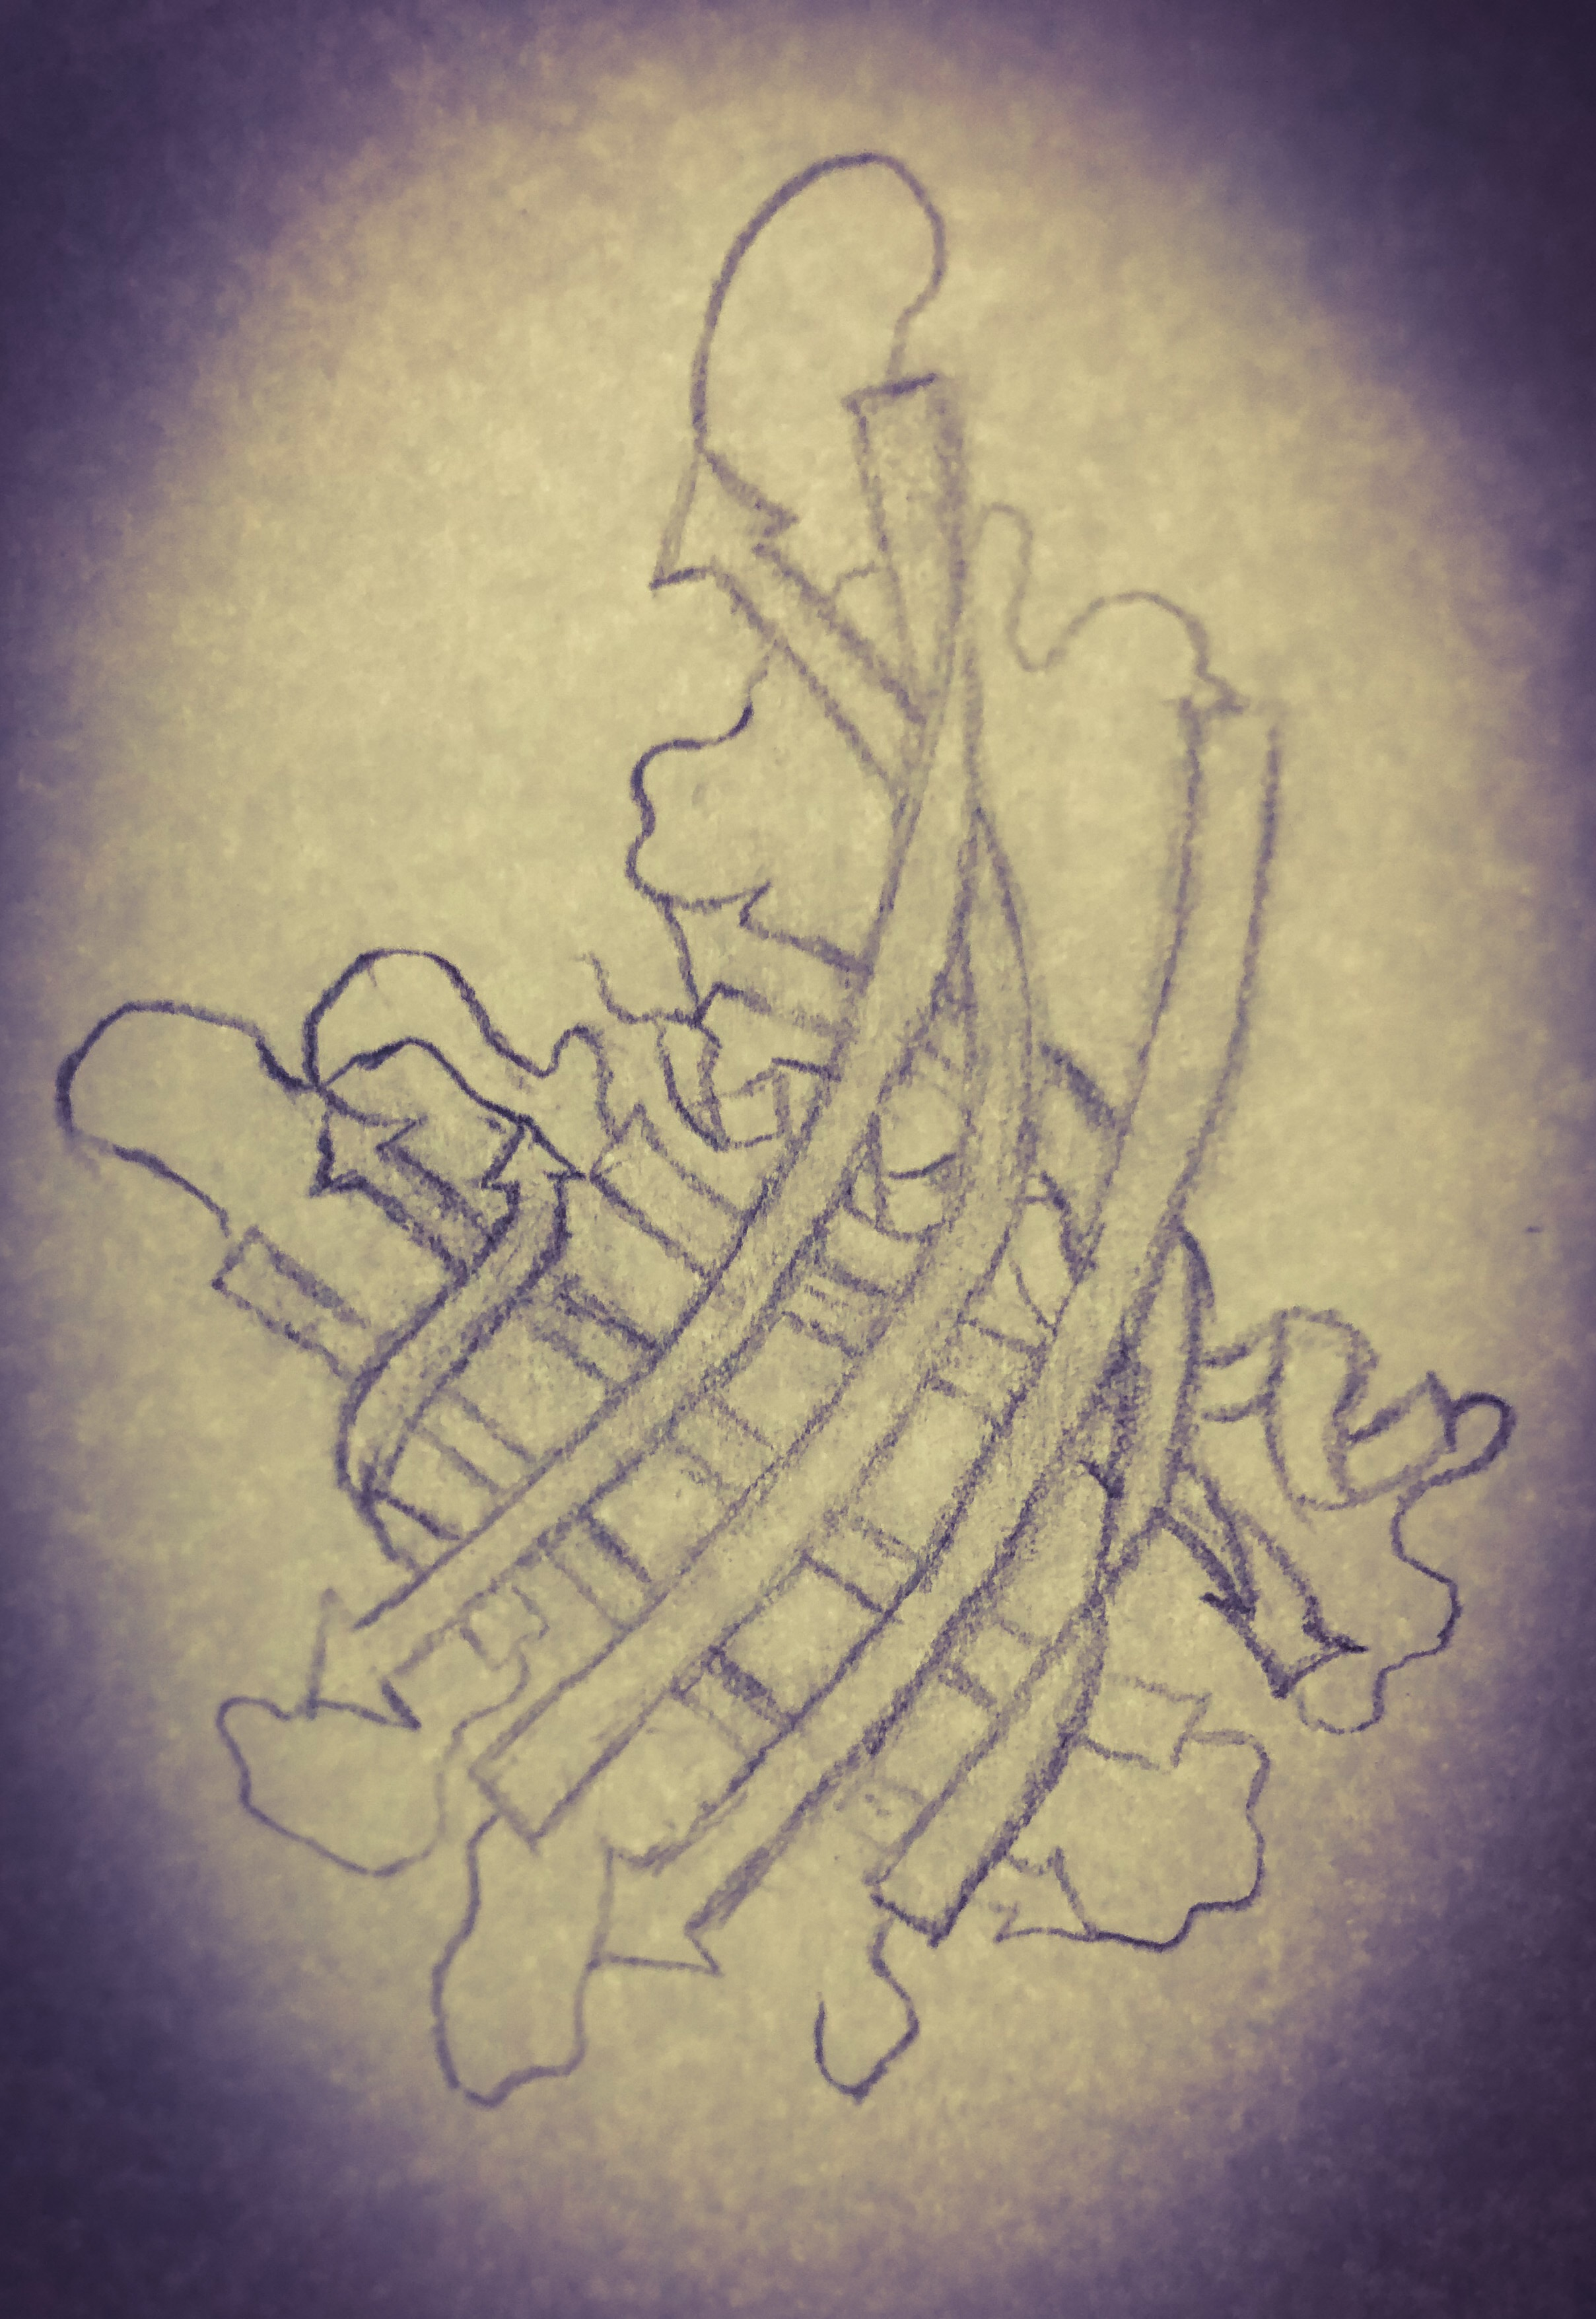
\includegraphics[width=\linewidth]{tertiary.jpg}
\caption{}\label{fig:fig_c}
\end{subfigure}
%
\begin{minipage}[t]{.5\textwidth}
\caption{Levels of protein structure (\subref{fig:fig_a}) $\alpha$-helix structure. (\subref{fig:fig_b}) parallel $\beta$-sheet structure.(\subref{fig:fig_c})tertiary structure comprised of a $\beta$-barrel and $\alpha$-helical moiety. }
\end{minipage}

\end{figure}
\end{comment}

\appendix


% Stuff at the end of the dissertation goes in the back matter
\backmatter
\bibliographystyle{plain} % Or whatever style you want like plainnat
\bibliography{library}

\end{document}
